\documentclass{exam}

\usepackage{graphicx} % Required for inserting images
\usepackage{amsmath}
\usepackage{titling}
\usepackage{caption}
\usepackage{dsfont}
\usepackage{amsfonts}
\usepackage{amsthm}
\usepackage{hyperref}
\usepackage[dutch]{babel}
\hypersetup{
    colorlinks,
    citecolor=black,
    filecolor=black,
    linkcolor=black,
    urlcolor=black
}

\renewcommand\maketitlehooka{\null\mbox{}\vfill}
\renewcommand\maketitlehookd{\vfill\null}
\newcommand{\RomanNumeralCaps}[1]{\MakeUppercase{\romannumeral #1}}
\counterwithin*{equation}{section}% Reset equation at \section
\counterwithin*{equation}{subsection}% Reset equation at \subsection
\counterwithin*{equation}{subsubsection}% Reset equation at \subsubsection

\usepackage[framemethod=TikZ]{mdframed}

\newcounter{prf}[section]\setcounter{prf}{0}
\renewcommand{\theprf}{\arabic{section}.\arabic{prf}}
\newenvironment{prf}[2][]{%
\refstepcounter{prf}%
\ifstrempty{#1}%
{\mdfsetup{%
frametitle={%
\tikz[baseline=(current bounding box.east),outer sep=0pt]
\node[anchor=east,rectangle,fill=red!20]
{\strut Bewijs~\theprf};}}
}%
{\mdfsetup{%
frametitle={%
\tikz[baseline=(current bounding box.east),outer sep=0pt]
\node[anchor=east,rectangle,fill=red!20]
{\strut Bewijs~\theprf:~#1};}}%
}\fi
\mdfsetup{innertopmargin=10pt,linecolor=red!20,%
linewidth=2pt,topline=true,%
frametitleaboveskip=\dimexpr-\ht\strutbox\relax
}
\begin{mdframed}[]\relax%
\label{#2}}{\vspace{0.25cm}\qed\end{mdframed}}
\newcounter{theo}[section]\setcounter{theo}{0}
\renewcommand{\thetheo}{\arabic{section}.\arabic{theo}}
\newenvironment{theo}[2][]{%
\refstepcounter{theo}%
\ifstrempty{#1}%
{\mdfsetup{%
frametitle={%
\tikz[baseline=(current bounding box.east),outer sep=0pt]
\node[anchor=east,rectangle,fill=cyan!20]
{\strut Definitie~\thetheo};}}
}%
{\mdfsetup{%
frametitle={%
\tikz[baseline=(current bounding box.east),outer sep=0pt]
\node[anchor=east,rectangle,fill=cyan!20]
{\strut Definitie~\thetheo:~#1};}}%
}%
\mdfsetup{innertopmargin=10pt,linecolor=cyan!20,%
linewidth=2pt,topline=true,%
frametitleaboveskip=\dimexpr-\ht\strutbox\relax
}
\begin{mdframed}[]\relax%
\label{#2}}{\vspace{0.25cm}\end{mdframed}}
\newcounter{lem}[section]\setcounter{lem}{0}
\renewcommand{\thelem}{\arabic{section}.\arabic{lem}}
\newenvironment{lem}[2][]{%
\refstepcounter{lem}%
\ifstrempty{#1}%
{\mdfsetup{%
frametitle={%
\tikz[baseline=(current bounding box.east),outer sep=0pt]
\node[anchor=east,rectangle,fill=green!20]
{\strut Wet~\thelem};}}
}%
{\mdfsetup{%
frametitle={%
\tikz[baseline=(current bounding box.east),outer sep=0pt]
\node[anchor=east,rectangle,fill=green!20]
{\strut Wet~\thelem:~#1};}}%
}%
\mdfsetup{innertopmargin=10pt,linecolor=green!20,%
linewidth=2pt,topline=true,%
frametitleaboveskip=\dimexpr-\ht\strutbox\relax
}
\begin{mdframed}[]\relax%
\label{#2}}{\vspace{0.25cm}\end{mdframed}}
\newcounter{ex}[section]\setcounter{ex}{0}
\renewcommand{\theex}{\arabic{section}.\arabic{ex}}
\newenvironment{ex}[2][]{%
\refstepcounter{ex}%
\ifstrempty{#1}%
{\mdfsetup{%
frametitle={%
\tikz[baseline=(current bounding box.east),outer sep=0pt]
\node[anchor=east,rectangle,fill=purple!20]
{\strut Voorbeeld~\theex};}}
}%
{\mdfsetup{%
frametitle={%
\tikz[baseline=(current bounding box.east),outer sep=0pt]
\node[anchor=east,rectangle,fill=purple!20]
{\strut Voorbeeld~\theex:~#1};}}%
}%
\mdfsetup{innertopmargin=10pt,linecolor=purple!20,%
linewidth=2pt,topline=true,%
frametitleaboveskip=\dimexpr-\ht\strutbox\relax
}
\begin{mdframed}[]\relax%
\label{#2}}{\vspace{0.25cm}\end{mdframed}}
\newcounter{pro}[section]\setcounter{pro}{0}
\renewcommand{\thepro}{\arabic{section}.\arabic{pro}}
\newenvironment{pro}[2][]{%
\refstepcounter{pro}%
\ifstrempty{#1}%
{\mdfsetup{%
frametitle={%
\tikz[baseline=(current bounding box.east),outer sep=0pt]
\node[anchor=east,rectangle,fill=lime!20]
{\strut Eigenschap~\thepro};}}
}%
{\mdfsetup{%
frametitle={%
\tikz[baseline=(current bounding box.east),outer sep=0pt]
\node[anchor=east,rectangle,fill=lime!20]
{\strut Eigenschap~\thepro:~#1};}}%
}%
\mdfsetup{innertopmargin=10pt,linecolor=lime!20,%
linewidth=2pt,topline=true,%
frametitleaboveskip=\dimexpr-\ht\strutbox\relax
}
\begin{mdframed}[]\relax%
\label{#2}}{\vspace{0.25cm}\end{mdframed}}
\newcounter{app}[section]\setcounter{app}{0}
\renewcommand{\theapp}{\arabic{section}.\arabic{app}}
\newenvironment{app}[2][]{%
\refstepcounter{app}%
\ifstrempty{#1}%
{\mdfsetup{%
frametitle={%
\tikz[baseline=(current bounding box.east),outer sep=0pt]
\node[anchor=east,rectangle,fill=magenta!20]
{\strut Toepassing~\theapp};}}
}%
{\mdfsetup{%
frametitle={%
\tikz[baseline=(current bounding box.east),outer sep=0pt]
\node[anchor=east,rectangle,fill=magenta!20]
{\strut Toepassing~\theapp:~#1};}}%
}\fi
\mdfsetup{innertopmargin=10pt,linecolor=magenta!20,%
linewidth=2pt,topline=true,%
frametitleaboveskip=\dimexpr-\ht\strutbox\relax
}
\begin{mdframed}[]\relax%
\label{#2}}{\vspace{0.25cm}\end{mdframed}}
\newcounter{summ}[section]\setcounter{summ}{0}
\renewcommand{\thesumm}{\arabic{section}.\arabic{summ}}
\newenvironment{summ}[2][]{%
\refstepcounter{summ}%
\ifstrempty{#1}%
{\mdfsetup{%
    frametitle={%
    \tikz[baseline=(current bounding box.east),outer sep=0pt]
    \node[anchor=east,rectangle,fill=violet!20]
    {\strut Samenvatting~\thesumm};}}
}%
{\mdfsetup{%
    frametitle={%
    \tikz[baseline=(current bounding box.east),outer sep=0pt]
    \node[anchor=east,rectangle,fill=violet!20]
    {\strut Samenvatting~\thesumm:~#1};}}%
}\fi
\mdfsetup{innertopmargin=10pt,linecolor=violet!20,%
    linewidth=2pt,topline=true,%
    frametitleaboveskip=\dimexpr-\ht\strutbox\relax
}
\begin{mdframed}[]\relax%
\label{#2}}{\vspace{0.25cm}\end{mdframed}}
\newcounter{vrg}[section]\setcounter{vrg}{0}
\renewcommand{\thevrg}{\arabic{section}.\arabic{vrg}}
\newenvironment{vrg}[2][]{%
\refstepcounter{vrg}%
\ifstrempty{#1}%
{\mdfsetup{%
    frametitle={%
    \tikz[baseline=(current bounding box.east),outer sep=0pt]
    \node[anchor=east,rectangle,fill=teal!20]
    {\strut Vergelijking~\thevrg};}}
}%
{\mdfsetup{%
    frametitle={%
    \tikz[baseline=(current bounding box.east),outer sep=0pt]
    \node[anchor=east,rectangle,fill=teal!20]
    {\strut Vergelijking~\thevrg:~#1};}}%
}
\mdfsetup{innertopmargin=10pt,linecolor=teal!20,%
    linewidth=2pt,topline=true,%
    frametitleaboveskip=\dimexpr-\ht\strutbox\relax
}
\begin{mdframed}[]\relax%
\label{#2}}{\vspace{0.25cm}\end{mdframed}}

\title{Natuurkunde voor Informatici}
\author{Pieter Vanderschueren}
\date{Academiejaar 2022-2023}

\begin{document}

\begin{titlingpage}
\maketitle
\end{titlingpage}


\newpage

%\vspace*{\fill}
%\begin{center}
%
%\section*{Introductie}
%\end{center}
%
%\noindent Deze samenvatting is gemaakt voor het vak 'Natuurkunde voor Informatici \RomanNumeralCaps{1}: mechanica en elektriciteit' en 'Natuurkunde  voor Informatici \RomanNumeralCaps{2}: magnetisme' gedoceerd door André Vantomme. Ik volg zo veel mogelijk de volgorde van de slides om het makkelijk te maken te volgen, maar ik gebruik de Giancoli voor praktisch alle informatie. Ook, deze samenvatting is eerder theoretisch. Voor voorbeelden, zie de slides of Giancoli.
%
%
%\vspace*{\fill}
%
%\newpage

\tableofcontents

\newpage

\vspace*{\fill}
\begin{center}
    
\section*{Inleiding}
\end{center}

\vspace*{\fill}

\newpage

\section{Vectoren}

\vspace{0.5cm}

\begin{theo}[Vector]{Vector}
    Een \textbf{Vector} is een grootheid met een grootte, net zoals een scalar, een richting en een zin.
    \begin{itemize}
        \item \textbf{Eenheidsvector:} een vector, meestal genoteerd als $ \hat{u} $ waarvan de lengte 1 is
        \item \textbf{Plaatsvector:} vector van een punt ten opzicht van het coördinatenstelsel
        \item \textbf{Relatieve positievector:} vector tussen twee punten
    \end{itemize}
\end{theo}

\begin{pro}[Eigenschappen van vectoren]{Eigenschappen van vectoren}
    Elke vector kan je zien als een som van meerdere vectoren, namelijk zijn coördinaatvectoren. We verklaren tweedimensionaal:
    
    \begin{equation*}
        \Vec{r} = r_x\hat{i} + r_y\hat{j}
    \end{equation*}

    \noindent Nu we dit weten kunen we som en verschil van twee vectoren gewoon zien als het optellen of aftrekken van de coördinaten. Deze coördinaten of vectorcomponenten kunnen we makkelijk berekenen, namelijk: 

    \begin{equation*}
        r_x = r\cos(\theta),\ r_y = r\sin(\theta)
    \end{equation*}
    
    \begin{center}
        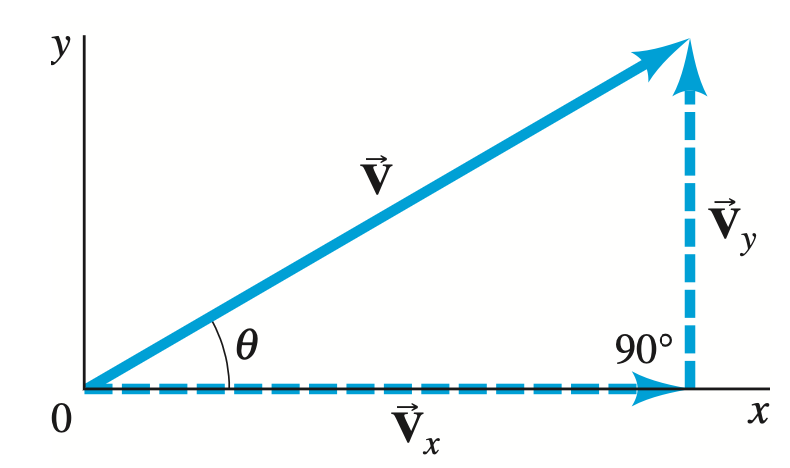
\includegraphics[scale = 0.4]{Images/Inleiding/Vectorcomponenten.png}
        \\
        ($\Vec{r} = \Vec{V}$ op de tekening)
    \end{center}
    
    \noindent Hieruit kunnen we het volgende afleiden:
    
    \begin{equation*}
        r = |r| = \sqrt{r_x^2 + r_y^2}, \ \theta = \tan^{-1}\dfrac{r_y}{r_x}
    \end{equation*}

    \noindent Deze samenvatting zal vaak gebruik maken van de volgende notatie met $\hat{u}$ een eenheidsvector met dezelfde richting als $\Vec{r}$:

    \begin{equation*}
        \Vec{r} = |r|\hat{u}
    \end{equation*}

    \noindent Dit volgt uit het feit dat 
    
    \begin{equation*}
        \hat{u} = \dfrac{\Vec{r}}{|r|}
    \end{equation*}
\end{pro}

\newpage

\begin{theo}[Dot product]{Dot product}
    Het dot product kan meetkundig geïnterpreteerd worden als de grootte van een vector maal de projectie van de andere vector. De formule is:
    \begin{equation*}
        \Vec{A} \cdot \Vec{B} = \sum_{i=1}^n a_ib_i = AB\cos{\theta}
    \end{equation*}
    \vspace{-0.5cm}
\end{theo}

\begin{pro}[Eigenschappen van het dot product]{pro - Dot product}
    \begin{itemize} 
    \item commutatief: $ A \cdot B = B \cdot A $
    \item distributief t.o.v. de optelling: $ A \cdot (B+C) = A \cdot B + A \cdot C $
\end{itemize}
\end{pro}

\begin{theo}[Vector product]{Vector product}
    De formule van het vector product geeft als uitkomst geen scalar, maar een gloednieuwe vector loodrecht op A en B . Hier deze formule:
    \begin{equation*}
        \Vec{A} \times \Vec{B} = \begin{vmatrix}
         \hat{i} & \hat{j} & \hat{k}\\ 
         A_x & A_y & A_z\\
         B_x & B_y & B_z  \end{vmatrix} = AB\sin(\theta) \hat{u}
    \end{equation*}
    met $\hat{u}$ een gerichte eenheidsvector loodrecht op het vlak.
\end{theo}

\begin{pro}[Eigenschappen van het vector product]{pro - Vector product}
    \begin{itemize} 
        \item \textbf{niet} commutatief: $ A \times B = \textbf{-}B \times A $
        \item distributief t.o.v. de optelling: $ A \times (B+C) = A \times B + A \times C $
    \end{itemize}
\end{pro}


\newpage

\vspace*{\fill}
\begin{center}
    
\section*{Kinematica}
\end{center}

\vspace*{\fill}

\newpage

\section{Vectoriële kinematica}

\vspace{0.5cm}

% \begin{app}[Vectoriële kinematica]{Vectoriële kinematica}

% % \begin{itemize}
% %     \item $ \Vec{r} = r\Vec{u} $
% %     \item $ \Vec{v} = \dfrac{d\Vec{r}}{dt} $
% %     \item $ \Vec{a} = \dfrac{d\Vec{v}}{dt} = \dfrac{d^2\Vec{r}}{dt^2}$
% % \end{itemize}

% % % \vspace{0.5cm}

% % % \noindent Hieruit volgt dan logischerwijs ook: 

% % % \vspace{0.5cm}

% \centering
% \def\arraystretch{2.5}
% \begin{tabular}{c|c|c}
%      & $ \Vec{v} $ & $ \Vec{a} $ \\ \hline 
%      gem &  $ \Vec{v}_{gem} = \dfrac{\Delta \Vec{r}}{\Delta t} $ & $ \Vec{a}_{gem} = \dfrac{\Delta \Vec{v}}{\Delta t} $ \\ \hline
%      ogb & $ \Vec{v}  
%      % \lim_{\Delta t \to 0} \dfrac{\Delta \Vec{r}}{\Delta t}  
%      = \dfrac{d\Vec{r}}{dt}$ & $ \Vec{a} = 
%      % \lim_{\Delta t \to 0}\dfrac{\Delta \Vec{v}}{\Delta t} = 
%      \dfrac{d\Vec{v}}{dt} $ 
% \end{tabular}

% \end{app}

\begin{pro}[Nuttige vergelijkingen bij constante versnelling]{Nuttige vergelijkingen bij constante versnelling}
    \vspace{-0.3cm}
    De volgende vergelijkingen kunnen gebruikt worden wanneer de versnelling constant is: $a = \dfrac{dv}{dt} = \text{cst}$:
    \begin{enumerate}
        \item $ r = r_{0} + v_{0}t + \tfrac{a}{2}t^2 = r_{0} + \overline{v}t$
        \item $ v = v_0 + at $ 
        \item $ \overline{v} = \dfrac{v + v_0}{2}$
        \item $ v^2 = v_0^2 + 2a(r-r_0) $
        % \begin{itemize}
        %     \item Dit kan je verkrijgen door (2) en (3) te substitueren in (1).
        % \end{itemize}
    \end{enumerate}
    \vspace{-0.3cm}
\end{pro}

\begin{app}[Projectielbeweging]{Projectielbeweging}
    Bij een projectielbeweging heeft het systeem horizontaal een constante snelheid (eenparige beweging) en verticaal een constante versnelling (eenparig versnelde beweging). In de volgende tabel zijn de formules samengevat: 

    \vspace{0.3cm}

    \begin{minipage}{.66\textwidth}
        \begin{center}
            \def\arraystretch{2}
            \begin{tabular}{c|c|c}
                & $x$ & $y$ \\ \hline
                $ r $ & $ x_0 + v_{x,0}t $ & $ y_0 + v_{y,0}t - \frac{gt^2}{2} $ \\ \hline
                $ v $ & $ v_{x,0} $ & $ v_{y,0} - gt $  \\ \hline
                $ a $ & $ 0 $ & $ -g $ 
            \end{tabular}
        \end{center}

        \vspace{0.3cm}
        % Ik ben ook niet trots op deze code, maar het werkt
        \hspace{-0.5cm}\noindent Hieruit kunnen we volgende formules halen: 

        \hspace{-0.5cm}\begin{minipage}{.43\textwidth}
            \begin{align*}
                x(t) &= v_{x,0}t \\
                y(t) &= v_{y,0}t - \frac{gt^2}{2}
            \end{align*}
        \end{minipage} \hspace{-0.5cm}$\longrightarrow$
        \begin{minipage}{.43\textwidth}
            \vspace{-0.2cm}
            \begin{equation*}
                y(x) = \frac{v_{y,0}}{v_{x,0}}x - \frac{g}{2v_{x,0}^2}x^2
            \end{equation*}
        \end{minipage}
        % \vspace{0.3cm}
    \end{minipage}
    \hspace{-1cm}\begin{minipage}{.4\textwidth}
        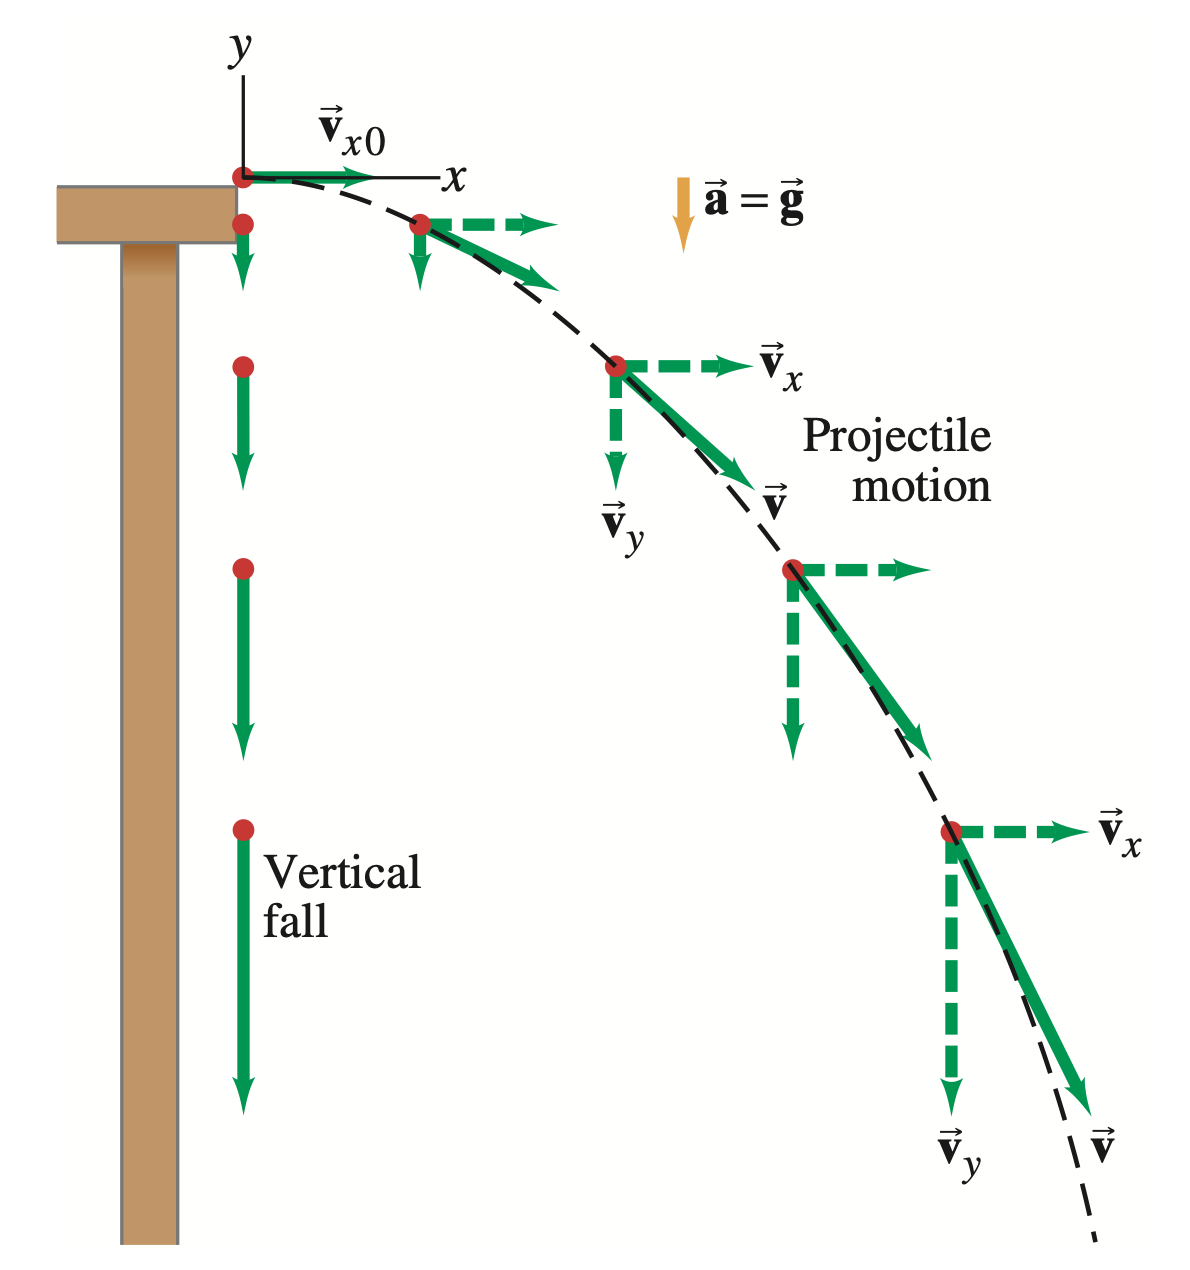
\includegraphics[scale = 0.255]{Images/Kinematica/Projectielbeweging.png}
    \end{minipage}

    \vspace{0.3cm}

    \noindent Deze formule bepaald de volgende parabole projectielbaan:
    \begin{center}
        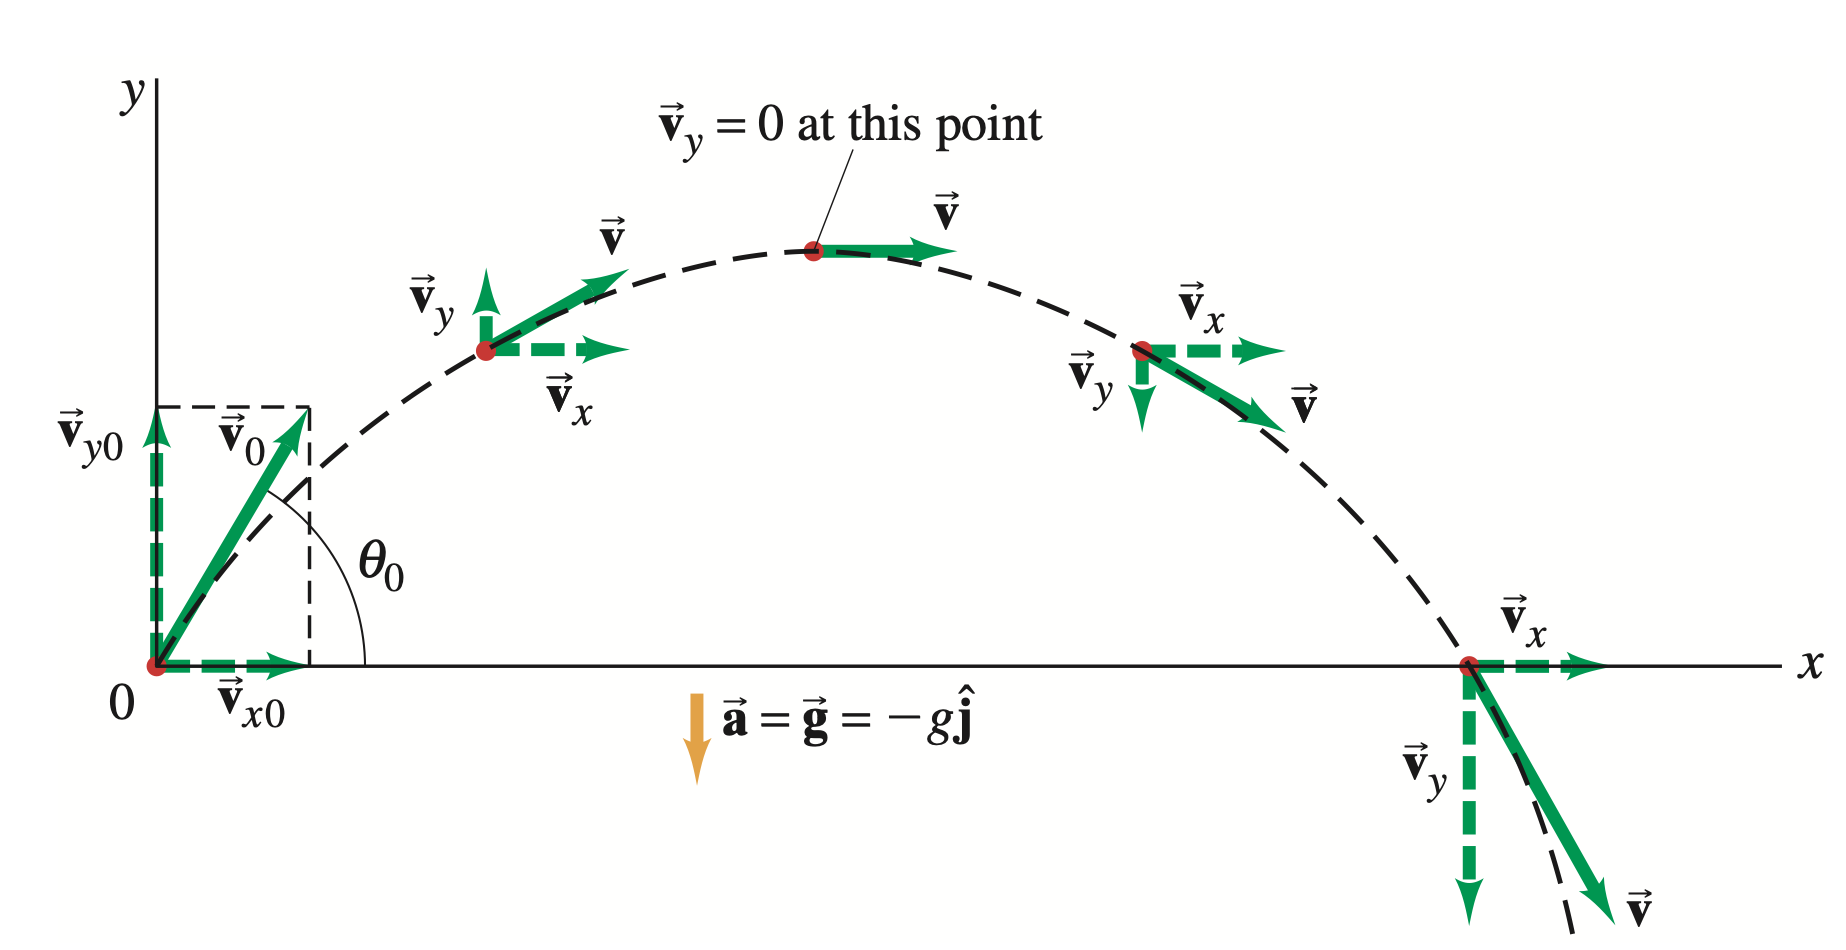
\includegraphics[scale = 0.28]{Images/Kinematica/Projectielbaan.png}
    \end{center}
\end{app}


\newpage

\vspace*{\fill}
\begin{center}
    
\section*{Dynamica}
\end{center}

\vspace*{\fill}

\newpage

\section{Newton's bewegingswetten}

\vspace{0.5cm}

\begin{theo}[Kracht]{Kracht}

Een kracht is een actie die de snelheid van een voorwerp verandert. Elke versnelling wordt dus veroorzaakt door een kracht. Er zijn twee soorten krachten: 

\begin{itemize}
    \item \textbf{Contactkrachten:} fysisch contact vindt plaats
    \item \textbf{Veldkrachten:} werken op een zekere afstand
\end{itemize}

\hspace{-0.65cm} Een kracht is een vectoriële grootheid en heeft dus een grootte, richting en zin.

\end{theo}

\begin{lem}[De eerste wet van Newton: de Inertiewet]{De eerste wet van Newton: de Inertiewet}

Een lichaam in rust (of in eenparige rechtlijnige beweging) zal in rust (eenparige rechtlijnige beweging) blijven tenzij er een uitwendige resulterende kracht inwerkt

    \begin{equation*}
        \sum_{i} \Vec{F}_i = 0 \to \Vec{a} = 0
    \end{equation*}

\hspace{-0.65cm} Een \textbf{inertiaalstelsel} is een referentiestelsel waarin de eerste wet van Newton geldt. De \textbf{inertie} wordt gegeven door de massa en beschrijft hoeveel weerstand dat een lichaam biedt tegen een verandering van zijn snelheid. 

    % \begin{equation*}
    %     \dfrac{m_1}{m_2} = \dfrac{a_2}{a_1}
    % \end{equation*}

\end{lem}

\begin{lem}[De tweede wet van Newton: de versnellingswet]{De tweede wet van Newton: de versnellingswet}

De versnelling van een voorwerp is recht evenredig met de nettokracht op het voorwerp en omgekeerd evenredig met het massa van het voorwerp. De richting van de versnelling is dezelfde als de richting van de nettokracht.

    \begin{equation*}
        \sum_{i} \Vec{F}_i = \Vec{F}_{net} = m\Vec{a} = m\dfrac{d\Vec{v}}{dt} = m\dfrac{d^2\Vec{r}}{dt^2}
    \end{equation*}

\end{lem}

\begin{lem}[De derde wet van Newton: de actie-reactiewet]{De derde wet van Newton: de actie-reactiewet}

Wanneer een voorwerp een kracht uitoefent op een ander voorwerp, dan oefent het ander voorwerp een kracht met dezelfde grootte en omgekeerde zin uit op het voorwerp.

    \begin{align*}
        \Vec{F}_{1 \to 2} &= -\Vec{F}_{2 \to 1} \\
       F_{1 \to 2} &= F_{2 \to 1}
    \end{align*}

\end{lem}

\newpage

\begin{theo}[Gravitatiekracht]{Gravitatiekracht}
Alle voorwerpen nabij het aardoppervlak vallen met dezelfde versnelling $ \Vec{g} $. De kracht bepaald door deze vernselling wordt de \textbf{gravitatiekracht} of \textbf{zwaartekracht} genoemd:

    \begin{equation*}
        \Vec{F}_G = m\Vec{g}
    \end{equation*}

\noindent Deze kracht is gericht naar het aardoppervlak toe en de grootte wordt het \textbf{gewicht} van een voorwerp genoemd. 

\end{theo}

\begin{theo}[Normaalkracht]{Normaalkracht}
    De \textbf{loodrechte} kracht die het contactoppervlak uitoefent op het voorwerp 
    \begin{equation*}
        F_N = F_{g,y} - \sum_{rest,y} F_{rest,y}
    \end{equation*}
    \noindent wordt de normaalkracht genoemd. De volgende figuren tonen enkele veelvoorkomende situaties voor de oefeningen:
    
    \begin{minipage}{.48\textwidth}
    
        \centering
        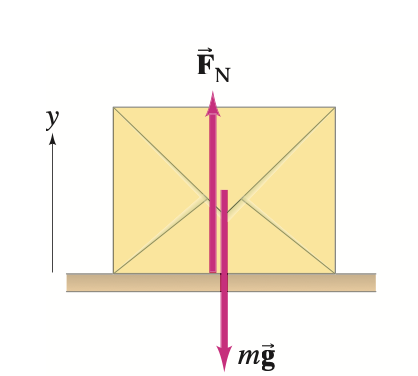
\includegraphics[scale = 0.7]{Images/Dynamica/Doos in rust.png}   
    
    \end{minipage} 
    \begin{minipage}{.48\textwidth}
    
        \centering
        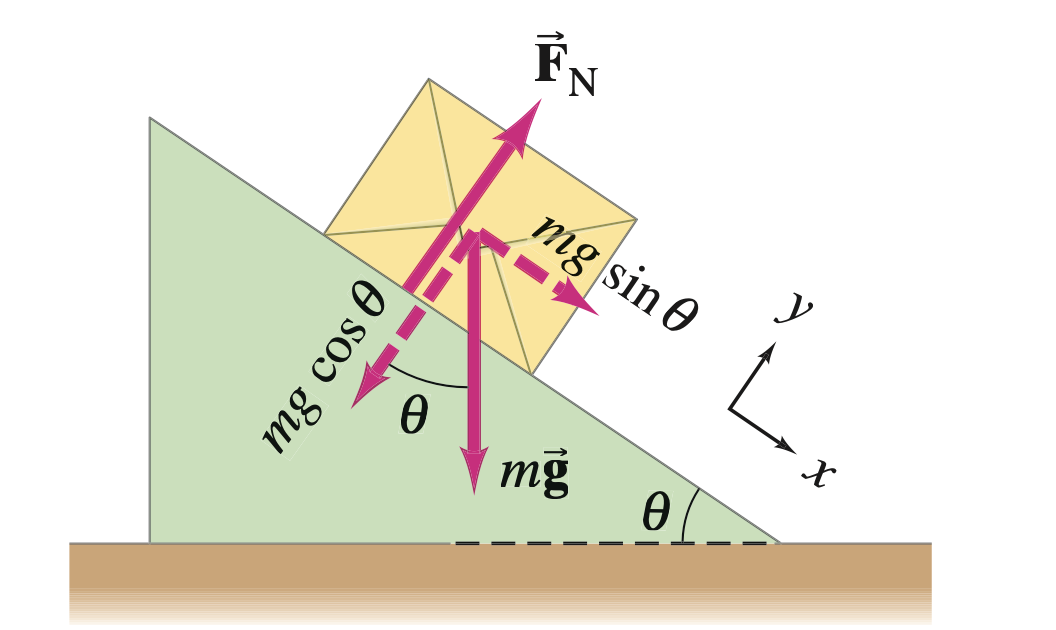
\includegraphics[scale = 0.35]{Images/Dynamica/Glijdende doos.png}
        
    \end{minipage}
    
    \vspace{0.25cm}
    
    \noindent De normaalkracht is dus afhankelijk van de gravitatiekracht van zijn grootte en zin, maar niet van zijn richting (zie de rechterfiguur). We kunnen dus \textbf{niet} zeggen dat het gravitatiekracht-normaalkracht paar een actie-reactie paar vormt. 
\end{theo}




\newpage

\section{De wetten van Newton: wrijving, cirkelbeweging, weerstandskrachten}

\vspace{0.5cm}

\begin{theo}[Wrijvingskracht]{Wrijvingskracht}

    De wrijvingkracht is de weerstand die het voorwerp ondervindt wanneer het over het oppervlak van een ander voorwerp beweegt. We bespreken 2 soorten wrijvingskrachten:
    
    \begin{itemize}
        \item \textbf{Kinetische:} $ F_k = \mu_kF_N$ met $ \mu_k $ de \textbf{kinetische} wrijvingscoëffiënt. Deze kracht is recht evenredig met de normaalkracht.
        \item \textbf{Statische:} $ F_s \leq \mu_sF_N$ met $ \mu_s $ de \textbf{statische} wrijvingscoëffiënt. Als deze drempelwaarde bereikt is, dan zal het object beginnen met bewegen en zal er sprake zijn van kinetische wrijving.
    \end{itemize}
    
    \noindent Er geldt dat het moeilijker is om een voorwerp te laten starten dan om een beweging verder te laten verlopen, of in formule vorm: 
    
    \begin{equation*}
        \mu_s > \mu_k
    \end{equation*} 

\end{theo}

% \begin{ex}[Voorbeeld: Wrijvingskracht]{Voorbeeld: Wrijvingskracht1}
%         \centering
%         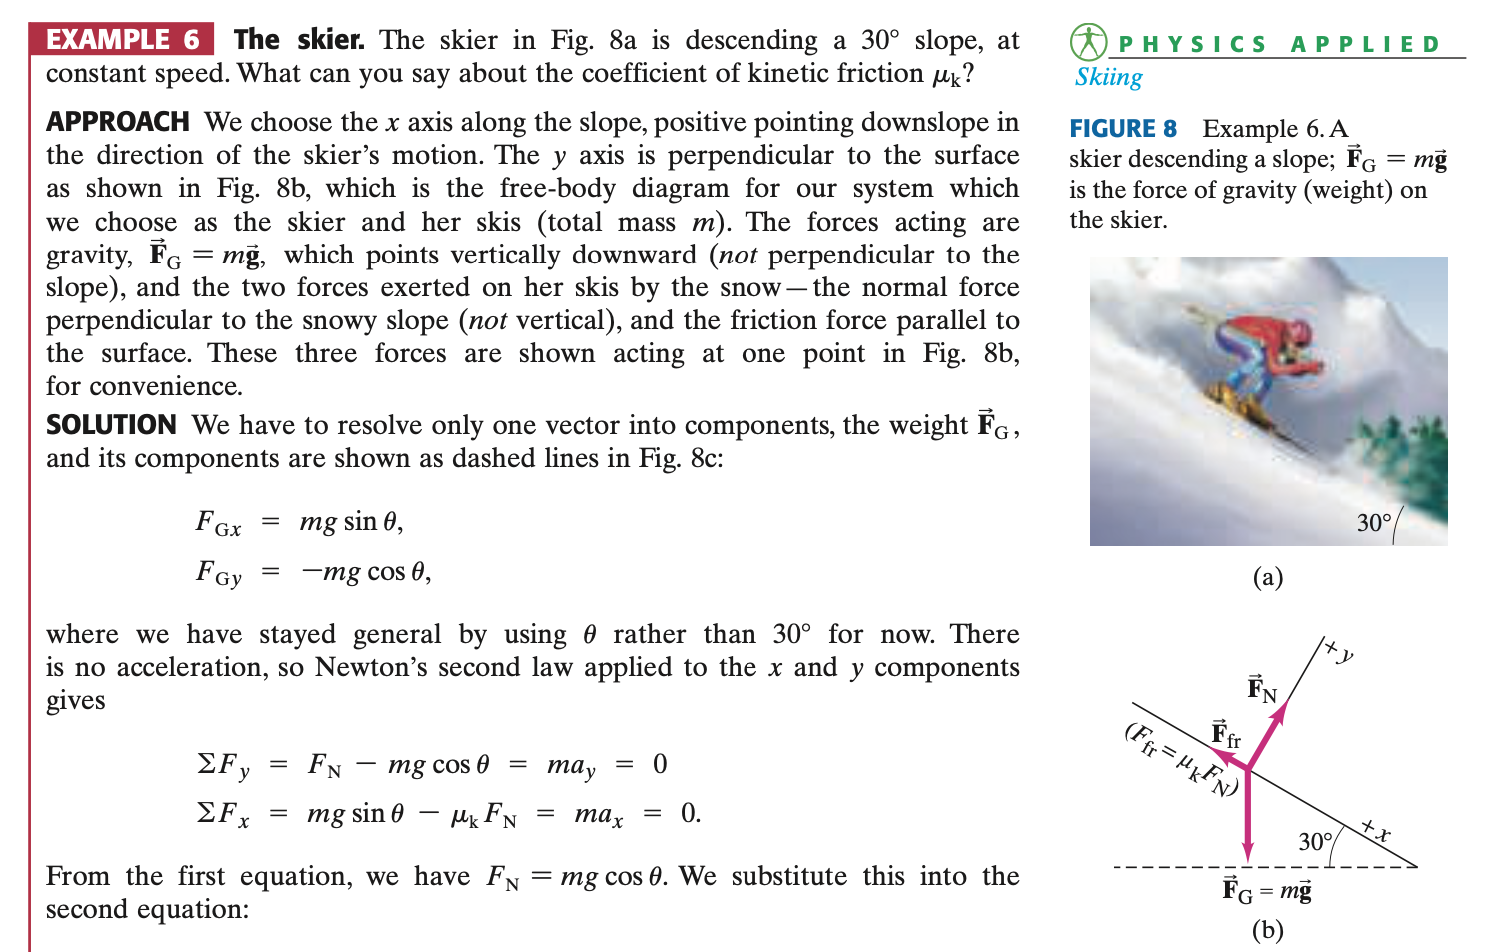
\includegraphics[scale = 0.6]{Examples/Dynamica/5.6.1.png}
%         \centering
%         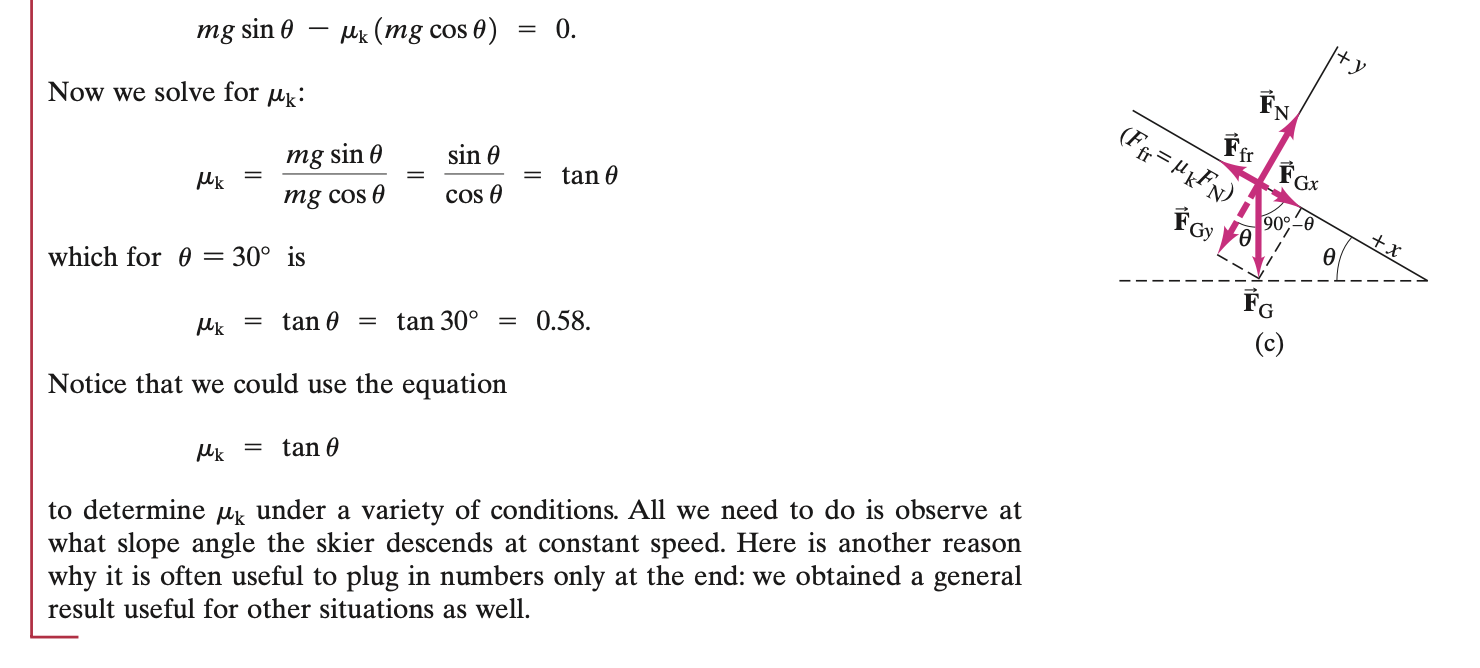
\includegraphics[scale = 0.6]{Examples/Dynamica/5.6.2.png}
%         \vspace{-0.5cm}
% \end{ex}

\begin{theo}[Kinematica van de eenparige cirkelbeweging]{Kinematica van de eenparige cirkelbeweging}
    Een voorwerp dat met een constante snelheid in een cirkel beweegt voert een \textbf{eenparig cirkelvormige beweging} uit. In dit soort beweging blijft de grootte van de snelheidsvector constant, maar verandert de richting continu, m.a.w. $ a \neq 0 $.

    \begin{minipage}{.55\textwidth}

        We berekenen de versnelling door te vertrekken van de formule:
        \begin{equation}
            \Vec{a} = \lim_{\Delta t \to 0} \dfrac{\Delta \Vec{v}}{\Delta t} = \dfrac{d\Vec{v}}{dt}
        \end{equation}
    
        Uit gelijkvormige driehoeken volgt: 
    
        \begin{equation}
            \dfrac{\Delta v}{v} \approx \dfrac{\Delta \ell}{r} \to \Delta v \approx \dfrac{v}{r}\Delta \ell
        \end{equation}

        % \begin{center}
        %     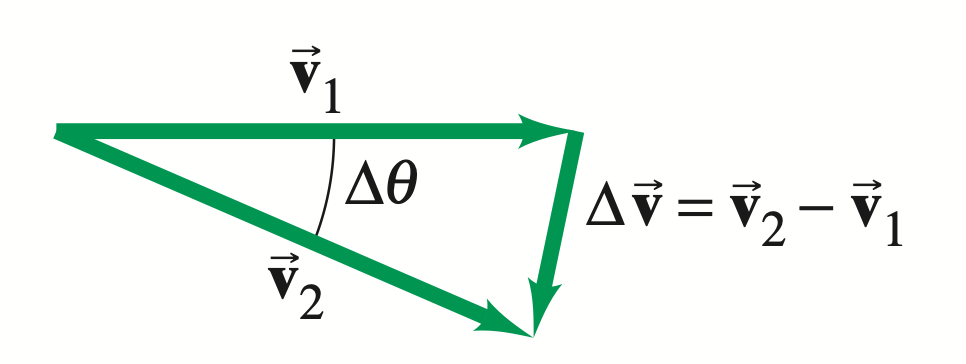
\includegraphics[scale = 0.25]{Images/Dynamica/Gelijkvormige driehoeken stap.png}
        % \end{center}
        
        Uit (1) en (2) volgt: 
    
        \begin{equation*}
            a_R = \lim_{\Delta t \to 0} \dfrac{\Delta v}{\Delta t} = \lim_{\Delta t \to 0} \dfrac{v}{r}\dfrac{\Delta \ell}{\Delta t}
        \end{equation*}
    
        
    \end{minipage} 
    \begin{minipage}{.41\textwidth}
            \centering
            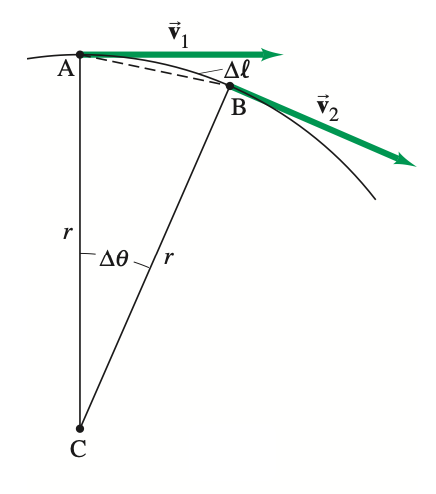
\includegraphics[scale = 0.35]{Images/Dynamica/Kinematica van de Cirkelbeweging.png}
            
    \end{minipage}
    
    \noindent Deze versnelling wordt de \textbf{centripetale versnelling genoemd} en is gericht naar het middelpunt van de cirkel. Deze wordt gegeven door de volgende formule: 
    
        \begin{equation*}
            a_R = \dfrac{v^2}{r}
        \end{equation*}
        
    \noindent De snelheid van een ECB wordt gegeven door de volgende formule: 
    
    \begin{equation*}
        v = \dfrac{2\pi r}{T}
    \end{equation*}
    
    \noindent Hierbij is T de periode, m.a.w. tijd nodig voor een complete omwenteling (Dimensie: s). De frequentie van de ECB, m.a.w het aantal omwentelingen per seconde (Dimensie: $ s^{-1} = Hz $), wordt gegeven door de volgende formule:
    
    \begin{equation*}
        f = \dfrac{1}{T} = \dfrac{v}{2\pi r} = \dfrac{\omega}{2\pi}
    \end{equation*}
\end{theo}

\begin{theo}[Dynamica van de eenparige cirkelbeweging]{Dyamica van de eenparige cirkelbeweging}
    De cirkelbeweging is een versnelde beweging, dus er is een resulterende kracht nodig om het voorwerp op de cirkelbaan te houden, namelijk de \textbf{centripetale kracht}:

    \begin{equation*}
        (\sum F)_R = ma_R = m\dfrac{v^2}{r}
    \end{equation*}
    
    \noindent Om een voorwerp op een cirkelbaan te houden is er een centripetale versnelling en zoals hierboven vermeld een centripetale kracht nodig, dus de $ F_{net} $ moet naar het midden van de cirkel gericht zijn. Als deze kracht er niet is, dan zal het volgens de \textbf{Inertiewet} rechtlijnig zich voortbewegen.
\end{theo}
 
\begin{theo}[Kinematica én Dynamica niet-eenparige cirkelbeweging]{Niet-eenparige cirkelbeweging}
    In dit soort beweging beweegt het voorwerp volgens een cirkelbaan, maar kan het versnellen. De totale vectoriele versnelling in dit soort beweging wordt gegeven door de volgende formule:
    \begin{equation*}
        \Vec{a} = \Vec{a}_{tan} + \Vec{a}_R 
    \end{equation*}

    \noindent Sinds $ \Vec{a}_R $ en $ \Vec{a}_{tan} $ altijd loodrecht op elkaar staan, geldt op eenderwelk ogenblik:
        \begin{equation*}
            a = \sqrt{a_{tan}^2 + a_R^2} \text{ met } a_R = \dfrac{v^2}{r} \text{ en } a_{tan} = \dfrac{dv}{dt}
        \end{equation*}

    \noindent De figuren tonen de tangentiele en centripetale krachten en versnellingen bij een niet-eenparige cirkelbeweging:
    
        \begin{center}
            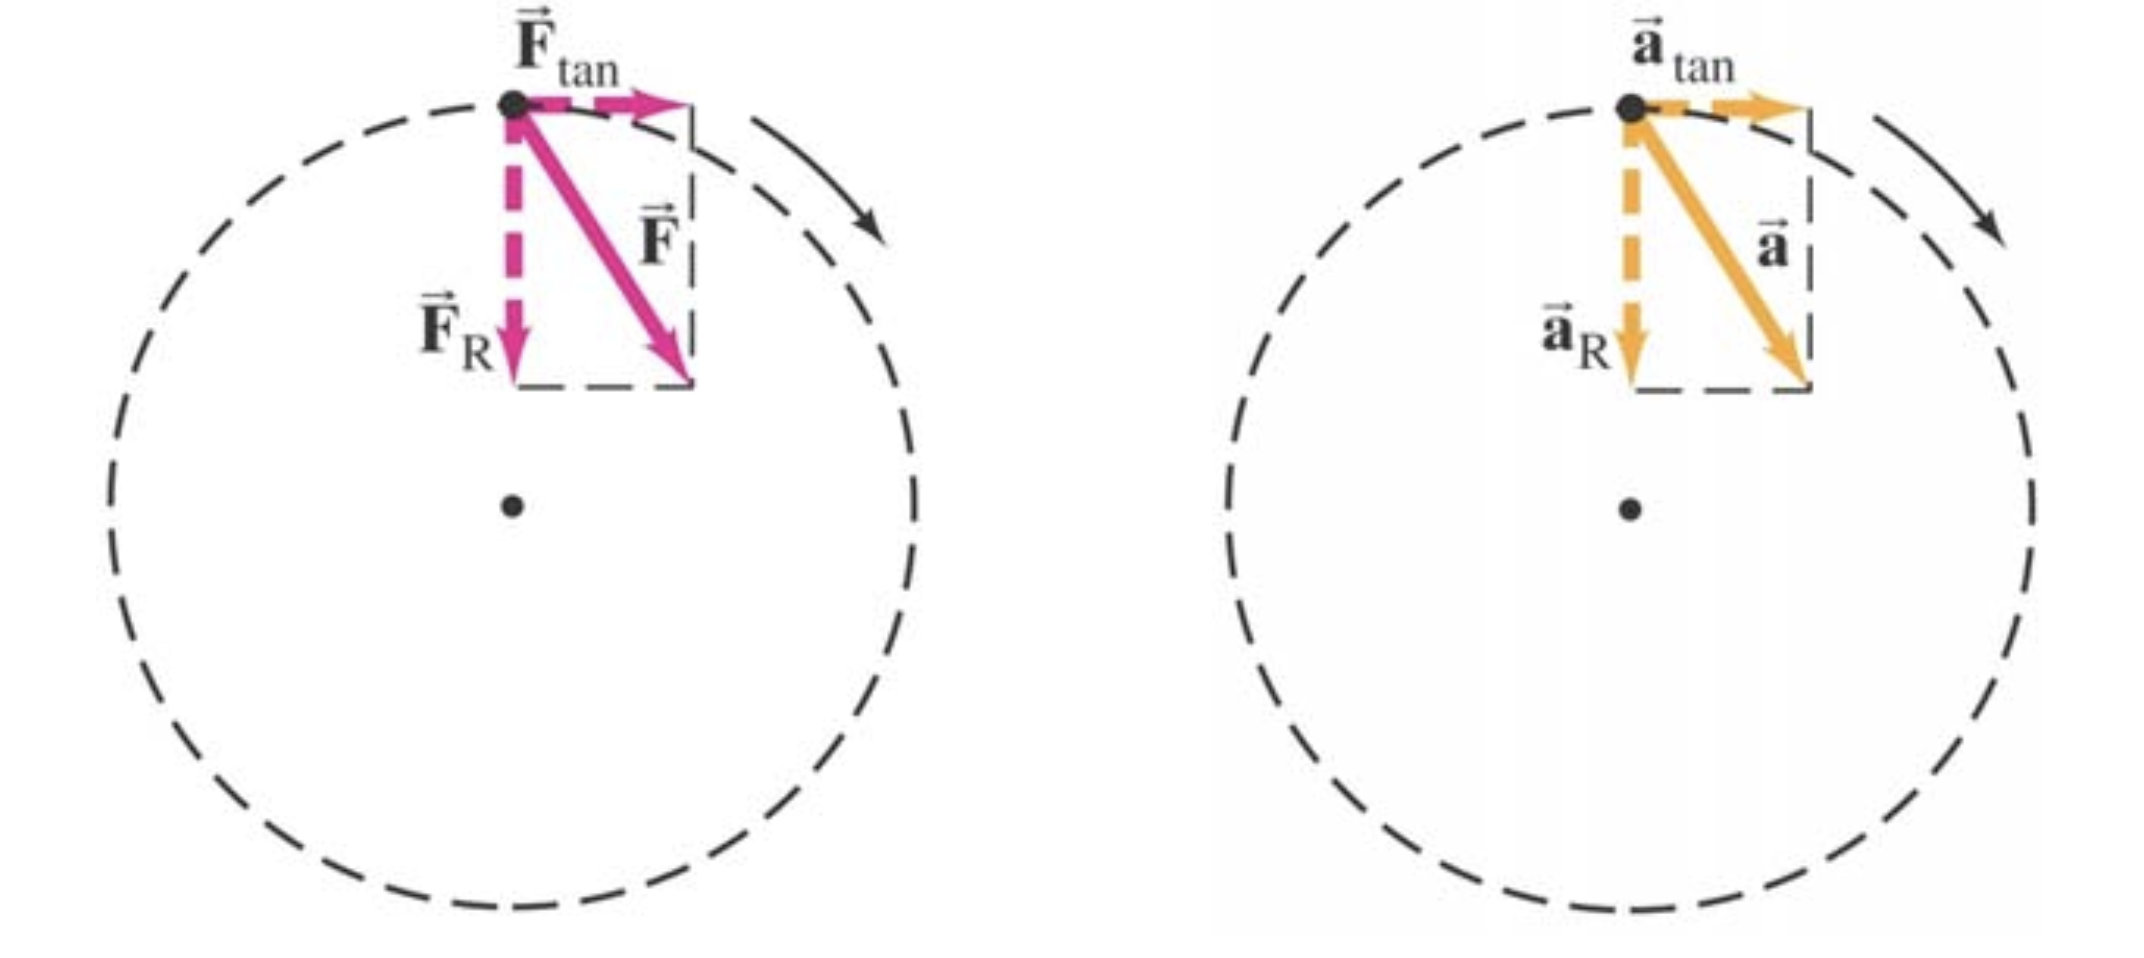
\includegraphics[scale = 0.20]{Images/Dynamica/Niet-Eenparige Cirkelbeweging.png} 
        \end{center}
\end{theo}

% \begin{ex}[Voorbeeld: Eenparige cirkelbeweging]{Eenparige cirkelbeweging}
%     \centering
%     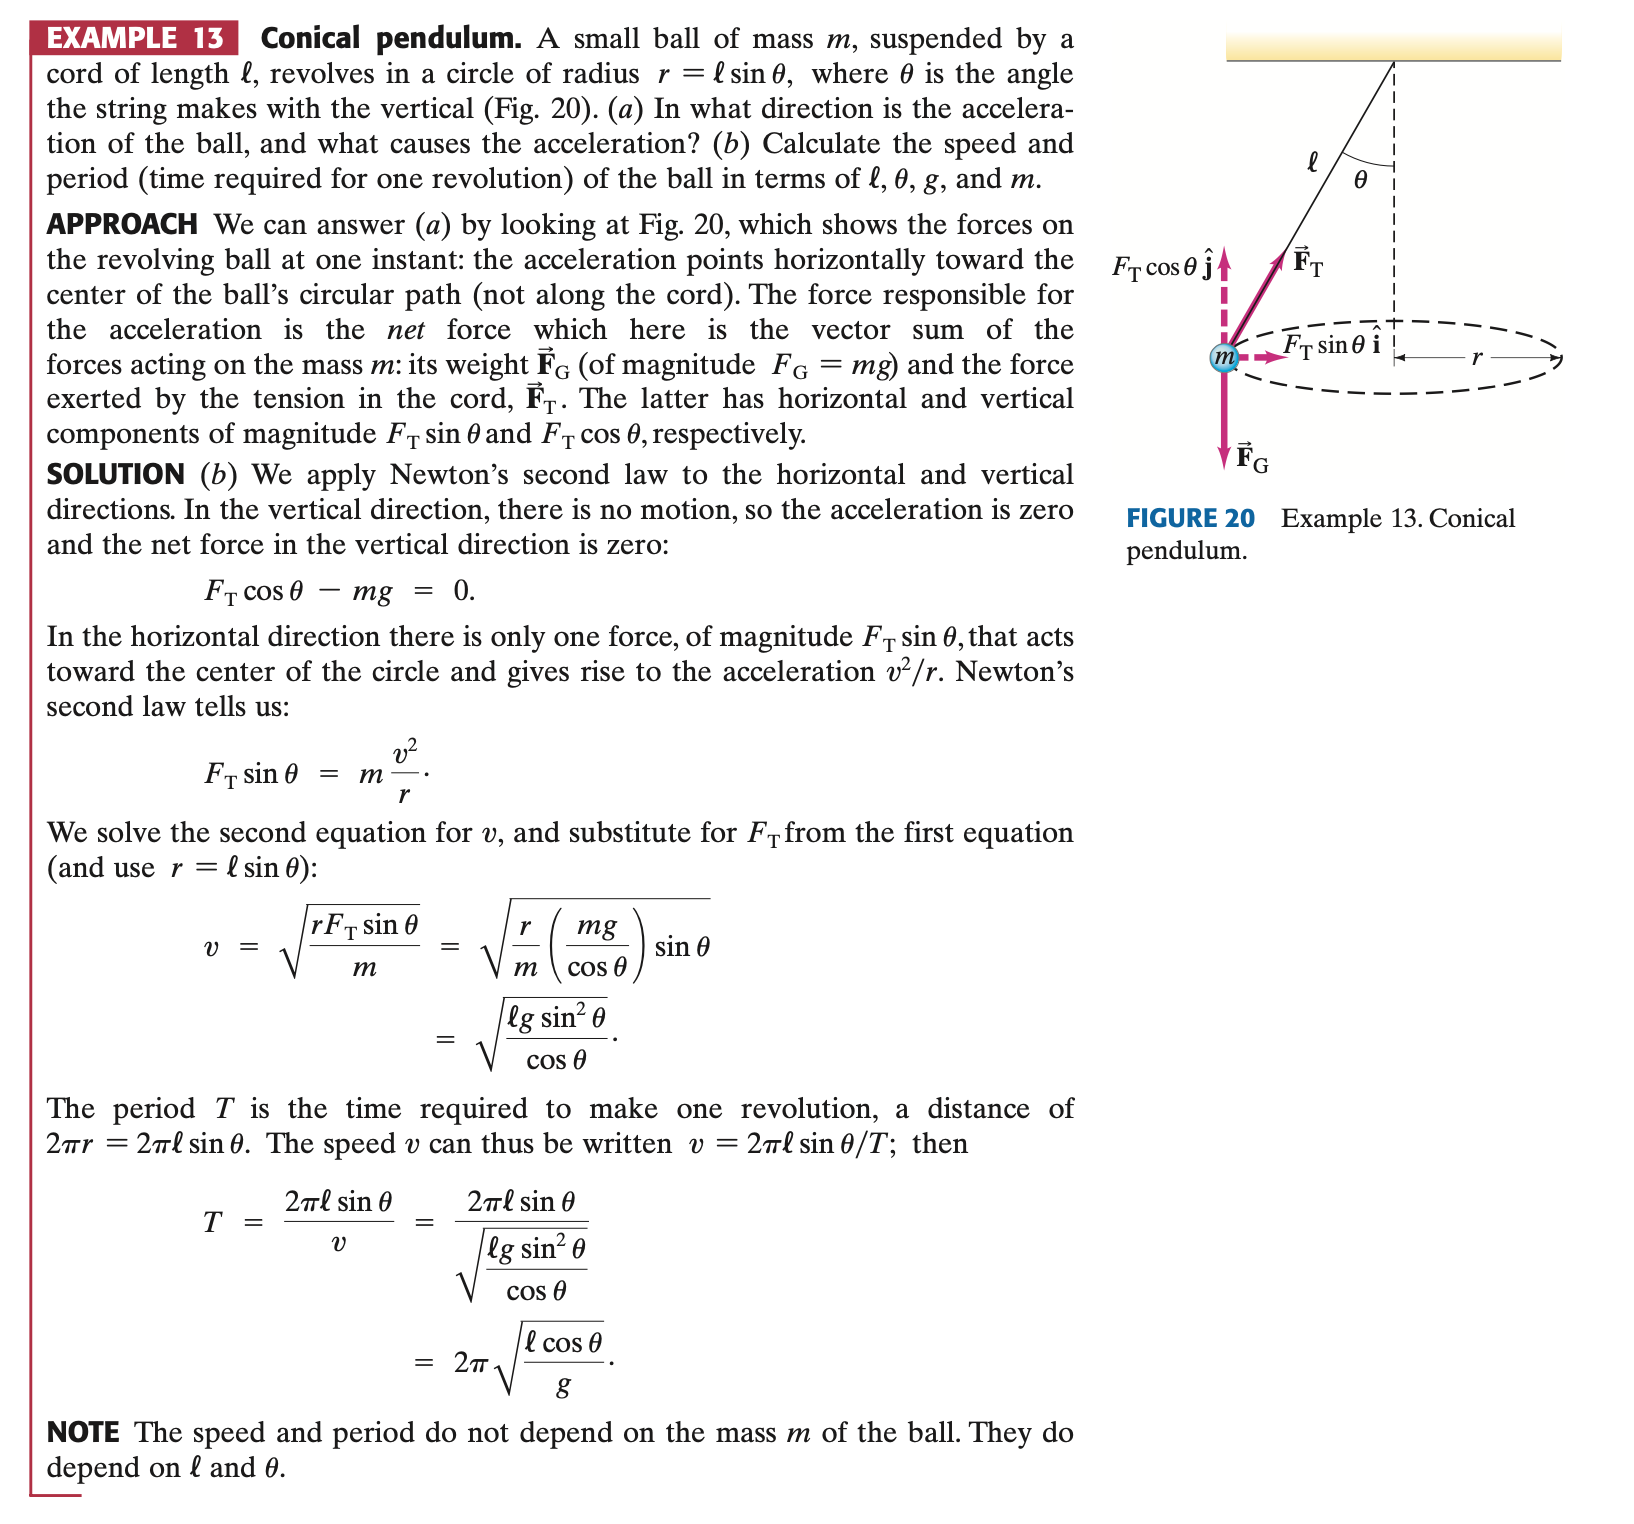
\includegraphics[scale = 0.55]{Examples/Dynamica/5.13.png}
% \end{ex}

\newpage

\section{De zwaartekracht en de synthese van Newton}

\vspace{0.5cm}

\begin{theo}[De wet van de universele zwaartekracht]{De wet van de universele zwaartekracht}

Elk deeltje in het heelal trekt elk ander deeltje aan met een kracht die recht evenredig is met het product van hun massa’s en omgekeerd evenredig met het kwadraat van de onderlinge afstand, in formulevorm:
 
 \begin{equation*}
     F_g = G\dfrac{m_1m_2}{r^2} \text{ met } G = 6.673 \times 10^{-11} \dfrac{Nm^2}{{kg}^2}
 \end{equation*}
 
\noindent We weten natuurlijk al uit voorgaande hoofdstukken wat de formule voor de zwaartekracht is nabij het aardoppervlak is, maar hoe komen we hieraan?

\begin{equation*}
    F_a = G\dfrac{mM_a}{(R_a+h)^2} \approx G\dfrac{mM_a}{r_a^2} = mG\dfrac{M_a}{r_a^2} \Rightarrow F_a = mg \text{ met } g = G\dfrac{M_a}{r_a^2}
\end{equation*}

% \noindent Als we nu stellen dat $ g = G\dfrac{M_a}{r_a^2} $, dan volgt:

% \begin{equation*}
%     F_a = mg
% \end{equation*}

\noindent \textbf{Let op:} De formule spreekt over twee puntmassas! Een macroscopisch voorwerp is een som (\textbf{integraal!}) over een zeer grote verzameling puntmassas, dus hoe moeten we het hier berekenen?
\begin{itemize}
    \item \textbf{Symmetrische bol:} alsof alle massa in het middelpunt zit
    \item \textbf{Symmetrische schil:} alsof alle massa in het middelpunt zit, én enkel kracht op massa buiten de schil
\end{itemize}

\end{theo}

\begin{app}[Satellieten]{Satellieten}

    Satellieten voeren een ECB uit rond de aarde. Er moet dus een centripetale kracht zijn die een satelliet op zijn baan houdt. Als we de tweede wet van newton zouden gebruiken vinden we in de radiale richting het volgende: 
    
    \begin{equation*}
        \sum F_R = G\dfrac{mM_a}{r_a^2} = m \dfrac{v^2}{r_a} \ met \ r_a = R_A + h_s
    \end{equation*}
    
    
    \noindent Hieruit volgt dat de tangentiêle snelheid, die de satteliet op zijn baan houdt, gelijk is aan het volgende:
    
    \begin{equation*}
        v = \sqrt{\dfrac{GM_a}{r}} = \sqrt{\dfrac{GM_a}{R_A + h_s}}
    \end{equation*}
    
    % \noindent \textbf{Opmerking:} een lagere/hogere baan heeft dus een hogere/lagere snelheid nodig

\end{app}

\begin{theo}[Gravitatieveld]{Gravitatieveld}
    
    % Volgens het veldconcept omringt een gravitatieveld elk voorwerp met massa en dit veld doordringt de hele ruimte. Een tweede voorwerp op een bepaalde plaats in de buurt van het eerste voorwerp ondervindt een kracht vanwege het daar aanwezige zwaartekrachtsveld. We kunnen het gravitatieveld definiëren als de gravitatiekracht per massa-eenheid op een willekeurig punt in de ruimte.
    
    Als we het gravitatieveld op een willekeurig punt willen meten, plaatsen we een kleine testmassa op dat punt en meten we de kracht die erop wordt uitgeoefend (waarbij we ervoor zorgen dat er alleen gravitatiekrachten werken). Dan is het gravitatieveld op dat singulier punt gedefinieerd als: 
    
    \begin{equation*}
        \Vec{g} = \dfrac{\Vec{F}}{m} = \dfrac{1}{m}G\dfrac{mM}{r^2}\hat{r} = -\dfrac{GM}{r^2}\hat{r} 
    \end{equation*}

\end{theo}

% \begin{ex}[Voorbeeld: Geostationaire satelliet]{Geostationaire satelliet}

%     \centering
%     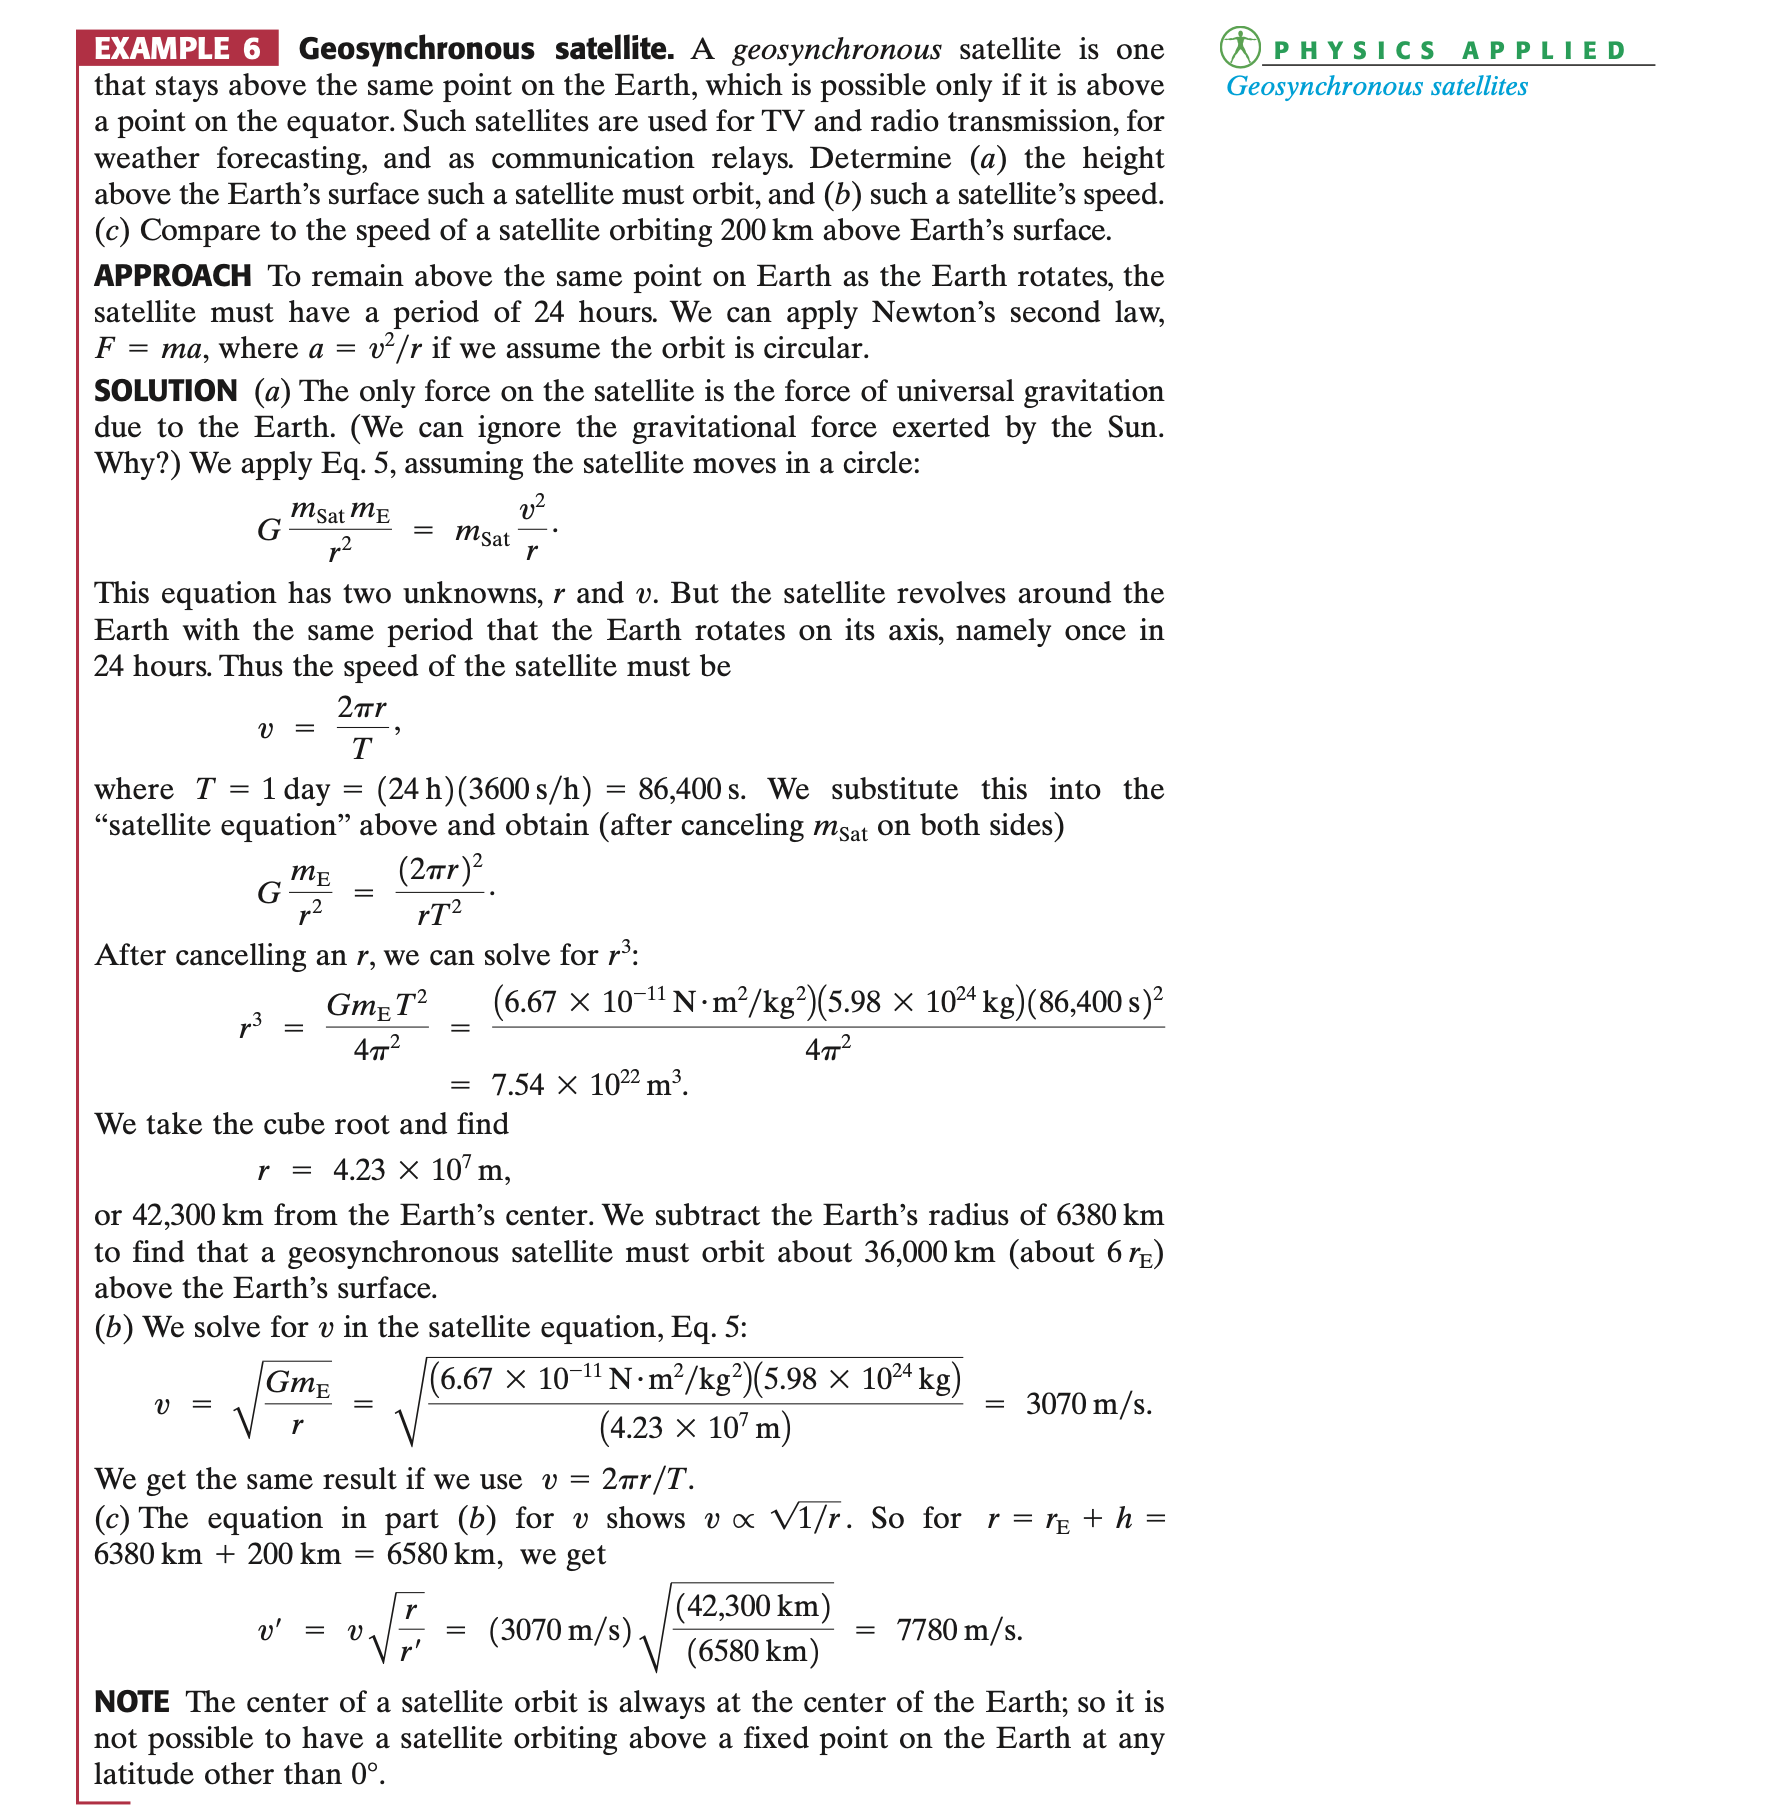
\includegraphics[scale = 0.5]{Examples/Dynamica/6.6.png}
    
% \end{ex}


\newpage

\section{Arbeid en energie}

\vspace{0.5cm}

\begin{theo}[Arbeid en energie]{Arbeid en energie}

    Arbeid is een scalaire grootheid voor het energietransfert, andersom is energie dan een scalaire grootheid voor de capaciteit om arbeid te leveren.

    \begin{itemize}
    
        \item{Arbeid en energie door een constante kracht}
        
            De arbeid geleverd door een constante kracht is gelijk aan de volgende formule:
            \begin{equation*}
                W = F_{||}d = Fdcos(\theta) = \Vec{F} \cdot \Vec{d}
            \end{equation*}
            \begin{center}
                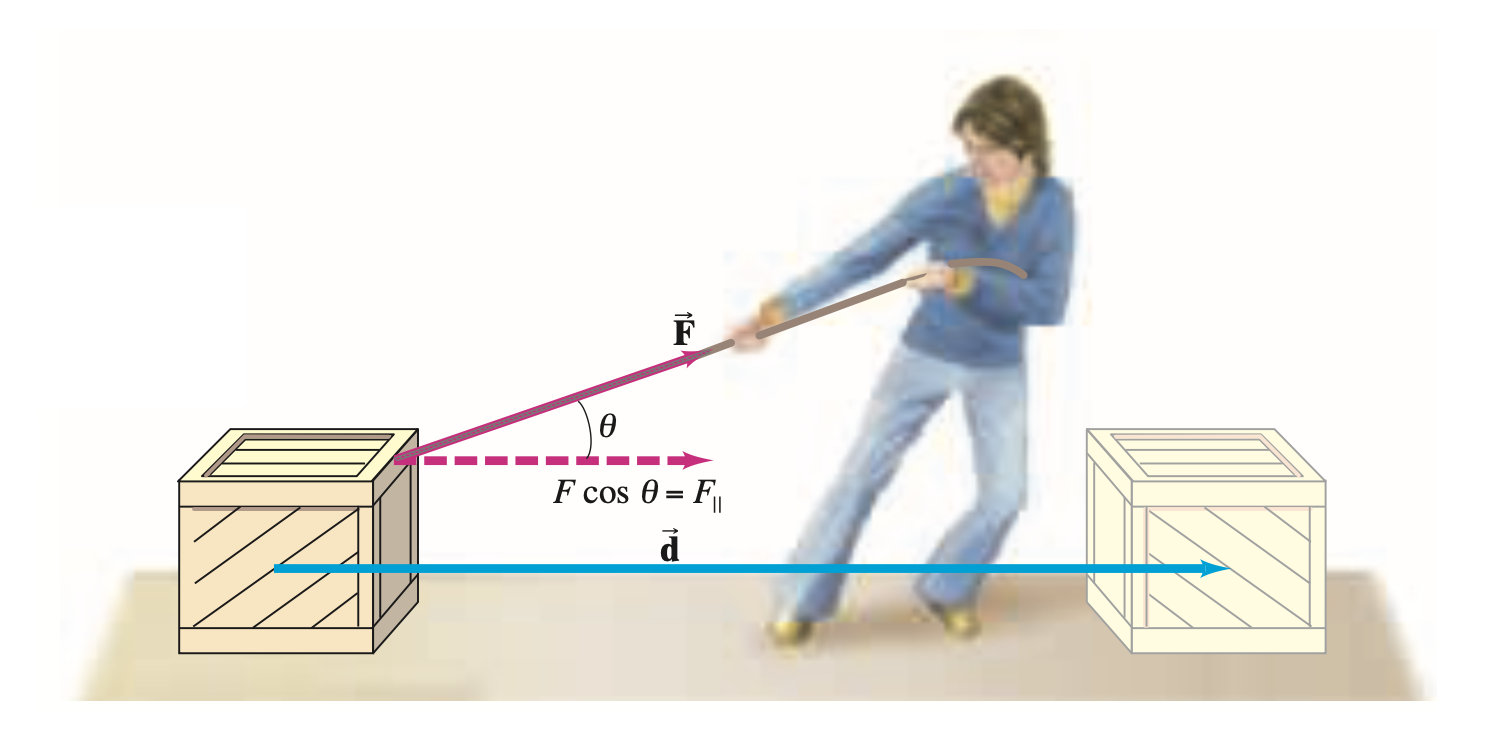
\includegraphics[scale = 0.15]{Images/Dynamica/Arbeid bij constante kracht.png}
            \end{center}
        \item{Arbeid en energie door een variabele kracht}
        
            Stel het voorwerp wordt bewogen door een variabele kracht over een pad $ a \to b $. We kunnen dit pad opsplitsen in infinitesimalen delen $ d\Vec{\ell} $. Als we nu integreren over het pad, dan krijgen we: 
            \begin{equation*}
                W = \int_{a}^{b}  F_{||}d\ell = \int_{a}^{b} F \cos\theta d\ell = \int_{a}^{b} \Vec{F} \cdot d\Vec{\ell}
            \end{equation*}
    \end{itemize}
\end{theo}

\begin{app}[Terugroepkracht van schroefveren]{Terugroepkracht van schroefveren}
    
    \begin{minipage}{.68\textwidth}
    
    Het uittrekken of samendrukken van een veer veroorzaakt een kracht, namelijk de terugroepkracht: 
    
    \begin{equation*}
        \Vec{F}_s = -k\Vec{x}
    \end{equation*}
    
    De arbeid geleverd door de veer hangt kunnen we ook berekenen:
    
    \begin{equation*}
        W_s = \int_0^x \Vec{F}_s \cdot d\Vec{x} = -\dfrac{1}{2}kx^2
    \end{equation*}

    Deze zal gelijk zijn bij samendrukken en uitrekken. \\

    \textbf{Opmerking}: de formule is geldig als de massa begint in de oorsprong en samengedrukt/uitgerokken wordt tot een punt x
    
    % Hieruit volgt dus ook dat $ W_{net} = 0 $ als we van $ -x \to x $, want:
    
    % \begin{equation*}
    %     W_{net} = W_{s,uit} + W_{s,sam} = -\dfrac{1}{2}kx^2 + \dfrac{1}{2}kx^2 = 0
    % \end{equation*}
    
    \end{minipage} 
    \begin{minipage}{.32\textwidth}
    
        \centering
        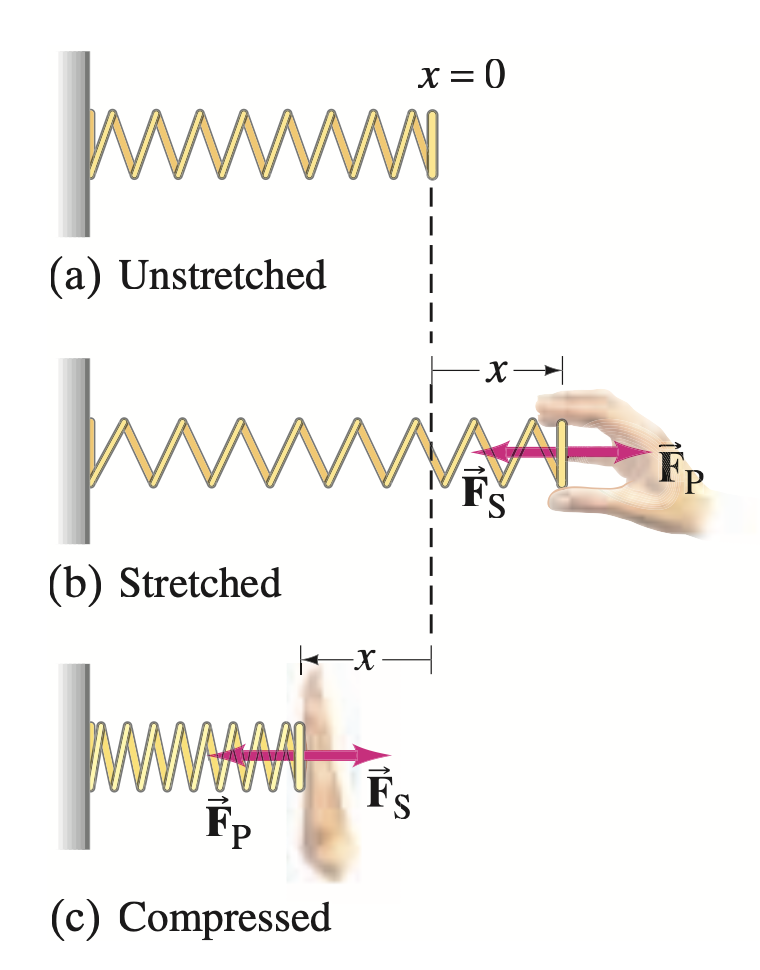
\includegraphics[scale = 0.325]{Images/Dynamica/Schroefveer.png}
        
    \end{minipage}
\end{app}

\begin{lem}[Arbeid - Kinetische energie theorema]{Arbeid - Kinetische energie theorema}

De netto-arbeid $ W_{net} $ geleverd door een voorwerp wordt bepaald door de netto-kracht $ F_{net} $. Stel we hebben een variabele (of een constante) kracht die inoefent op een voorwerp, we berekenen nu de netto-arbeid: 

\begin{align*}
    W_{net} &= \int_i^f \Vec{F}_{net} \cdot d\Vec{\ell} \\
            &= \int_i^f F_{||}d\ell \\
 \hspace{6.5cm} &= \int_i^f m\dfrac{dv}{dt}d\ell \qquad \qquad \ \ (F_{||} = ma_{||} = m\dfrac{dv}{dt}) \\
            &= \int_i^f mvdv \qquad \qquad \quad \  (v=\dfrac{d\ell}{dt}) \\
\hspace{6.5cm} &= \dfrac{1}{2}mv_f^2 - \dfrac{1}{2}mv_i^2 \quad \quad (F_{net} = ma, \ a = \dfrac{v_2^2 - v_1^2}{2d}) \\ 
            &= \Delta K 
\end{align*}

\noindent Wat we hierboven bewezen hebben is het \textbf{Arbeid - Kinetische energie theorema}, in woorden: 

\vspace{0.3cm} \noindent  "Wanneer de enige verandering in het systeem de snelheid is, dan is de arbeid verricht door de nettokracht gelijk aan de verandering in kinetische energie van het systeem."

\end{lem}


\newpage

\section{Behoud van energie}

\vspace{0.5cm}

\begin{theo}[Conservatieve en niet-conservatieve krachten]{Conservatieve en niet-conservatieve krachten}
    Een \textbf{conservatieve kracht} is een kracht waarbij de netto-arbeid geleverd door deze kracht nul is bij een gesloten baan, onafhankelijk is van de afgelegde weg. Bijvoorbeeld: 
    \begin{itemize}
        \item de gravitatiekracht: $ \Vec{F}_g = m\Vec{g} $      
        % \\
        % \begin{minipage}{.48\textwidth}
        %     \vspace*{\fill}
        %     \begin{align*}
        %         W &= -\int_a^b mg\hat{k}d\Vec{r} \\
        %           &= -mg\int_a^b\hat{k}(dx\hat{i}+dy\hat{j}+dz\hat{k}) \\
        %           &= -mg\int_a^bdz \\
        %           &= -mg(z_b - z_a)
        %     \end{align*}
        %     \vspace*{\fill}
            
        % \end{minipage} 
        % \begin{minipage}{.25\textwidth}
        
        %     \centering
        %     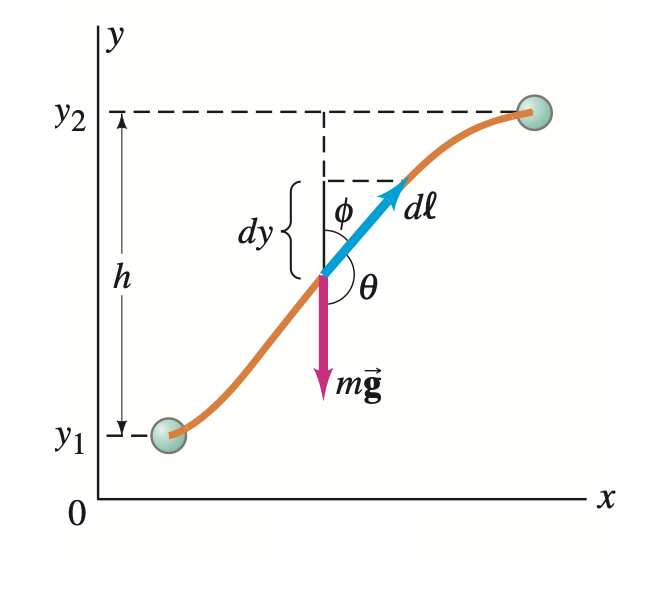
\includegraphics[scale = 0.225]{Images/Dynamica/ConservatieveZwaartekracht.png}
            
        % \end{minipage}
        \item de veerkracht: $ \Vec{F}_s = -k\Vec{x} $
    \end{itemize}
    
    \noindent Een \textbf{niet-conservatieve kracht} is een kracht waarbij de netto-arbeid geleverd door deze kracht afhankelijk is van de gevolgde weg 
    % \\ \\
    % \begin{minipage}{.44 \textwidth}
    %         \noindent\fbox{\parbox{\textwidth}{
    %         A crate is pushed slowly at constant speed across a rough floor
    %         from position 1 to position 2 via two paths: one straight and one curved. The pushing force $ F_P $ is in the direction of motion at each point. (The friction force opposes the motion.) Hence for a constant magnitude pushing force, the work it does is $ W = F_Pd$ , so if $ d $ is greater (as for the curved path), then $ W $  is greater. The work done does not depend only on points 1 and 2; it also depends on the path taken.}}       
    % \end{minipage} 
    % \begin{minipage}{.54\textwidth}
    %     \centering
    %     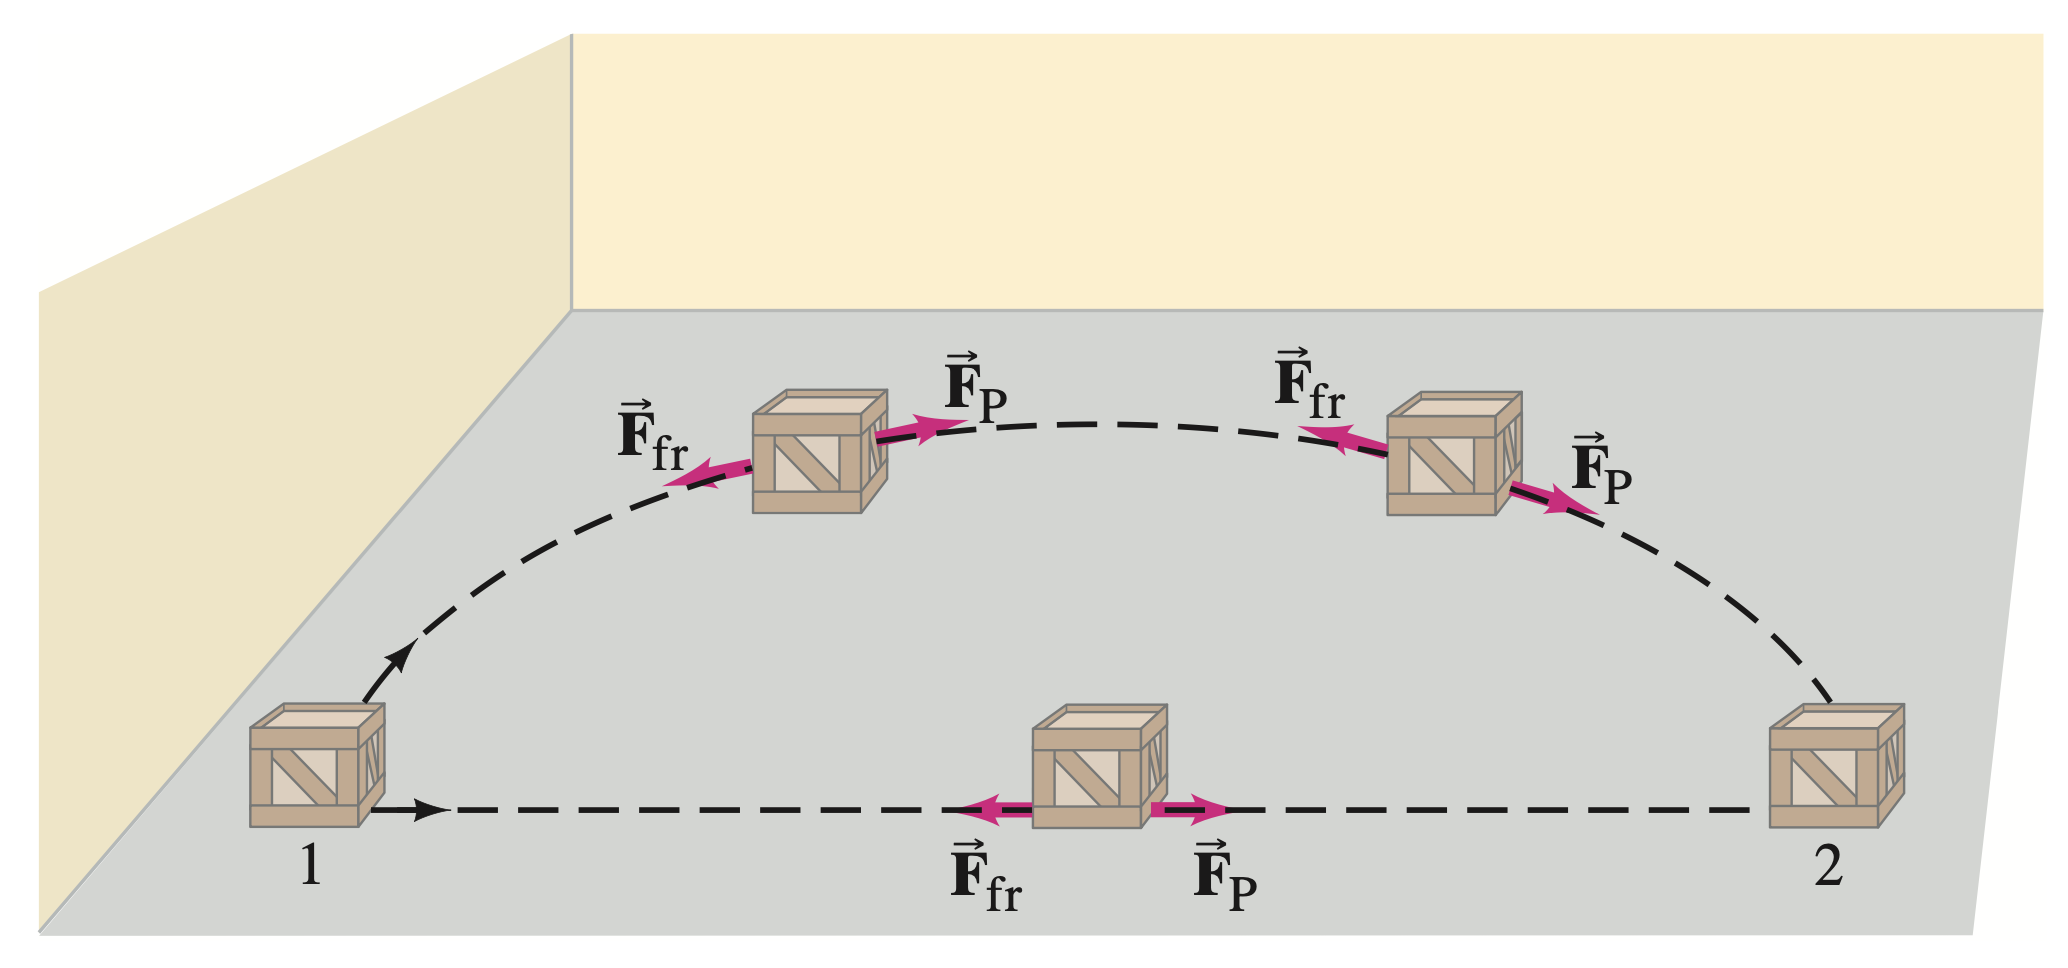
\includegraphics[scale = 0.2]{Images/Dynamica/NietConservatief.png}
    % \end{minipage}
\end{theo}

% \begin{theo}[Niet-conservatieve kracht]{Niet-conservatieve kracht}
%     Een \textbf{niet-conservatieve kracht} is een kracht waarbij de netto-arbeid geleverd door deze kracht afhankelijk is van de gevolgde weg \\ \\
%         \begin{minipage}{.44 \textwidth}
%                 \noindent\fbox{\parbox{\textwidth}{
%                 A crate is pushed slowly at constant speed across a rough floor
%                 from position 1 to position 2 via two paths: one straight and one curved. The pushing force $ F_P $ is in the direction of motion at each point. (The friction force opposes the motion.) Hence for a constant magnitude pushing force, the work it does is $ W = F_Pd$ , so if $ d $ is greater (as for the curved path), then $ W $  is greater. The work done does not depend only on points 1 and 2; it also depends on the path taken.}}       
%         \end{minipage} 
%         \begin{minipage}{.54\textwidth}
%             \centering
%             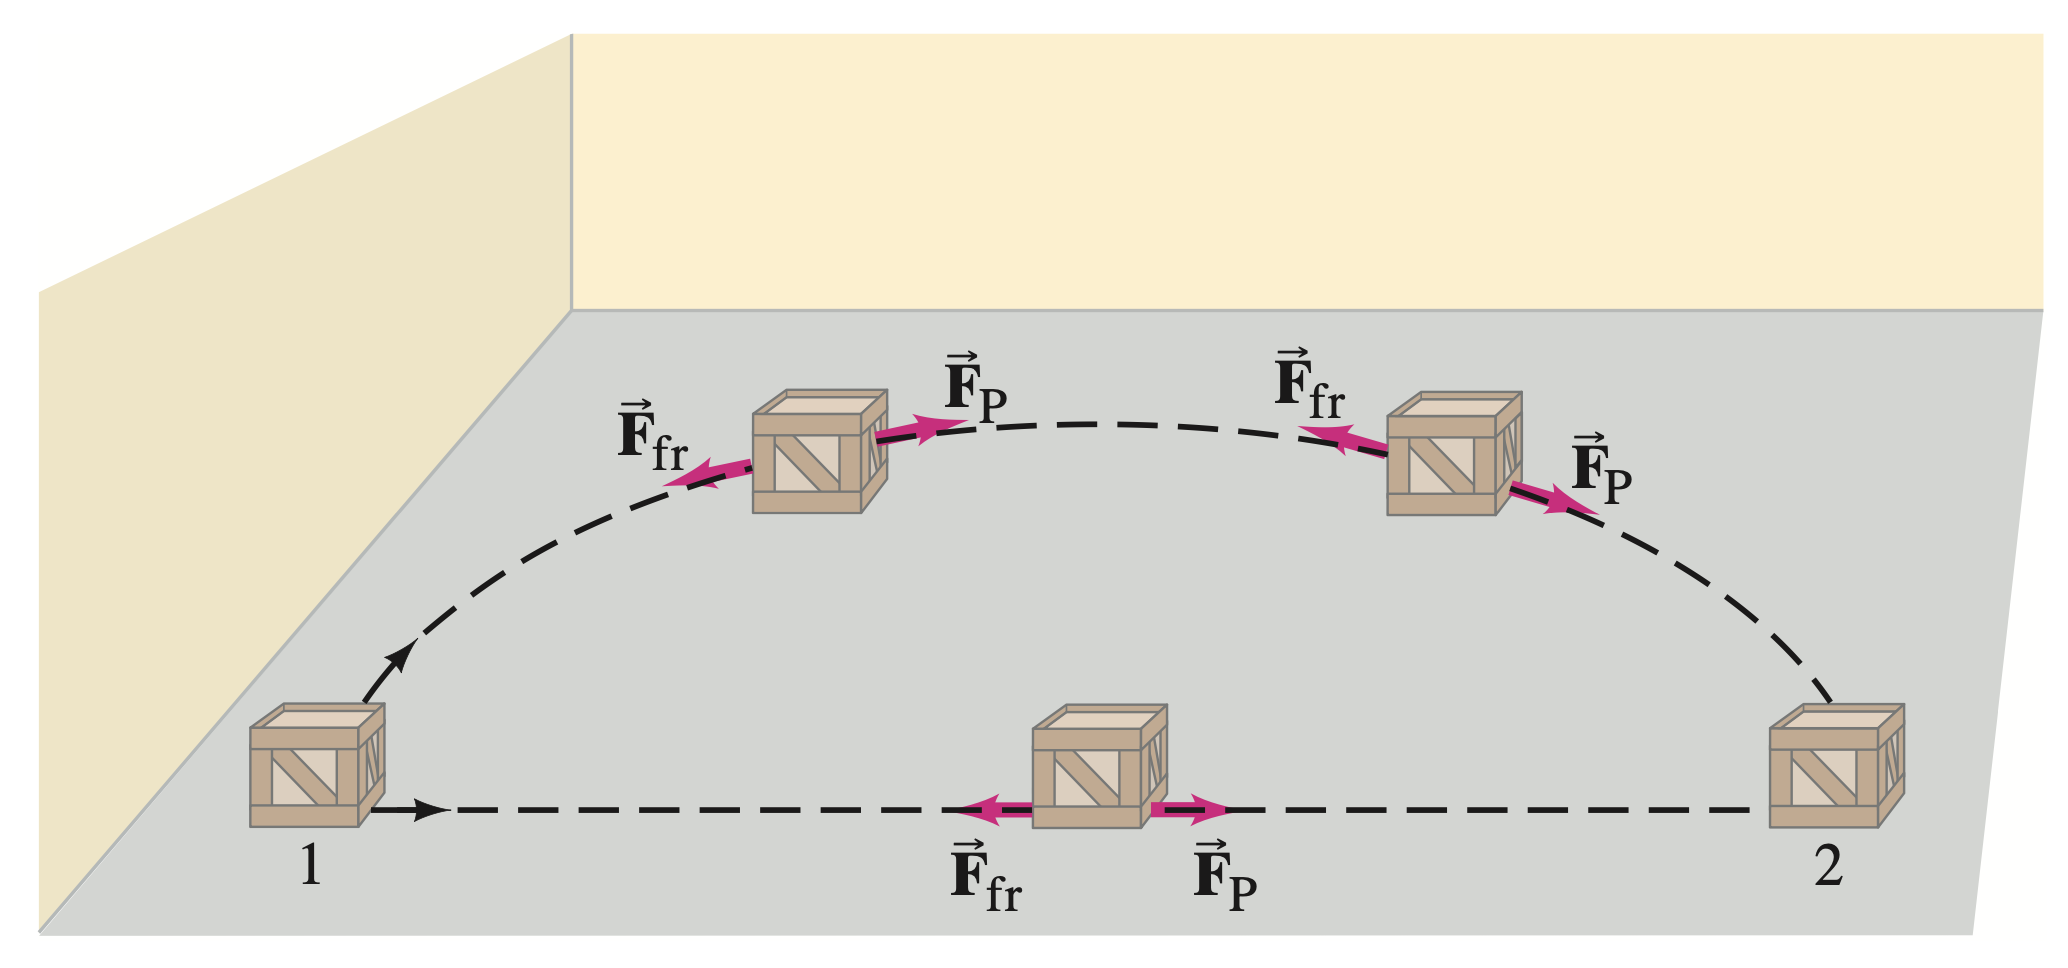
\includegraphics[scale = 0.2]{Images/Dynamica/NietConservatief.png}
%         \end{minipage}
% \end{theo}

\begin{theo}[Potentiële energie]{Potentiële energie}
    
    % Vanaf dit deelhoofdstuk spreken we ook van \textbf{potentiele energie} $ U $, wat geassocieerd wordt met krachten die afhangen van positie of afhangen van omgeving, dus: conservatieve krachten. \\
    
    \noindent De arbeid geleverd door een conservatieve kracht is gelijk aan het tegengestelde van de verandering in potentiële energie: 
        \begin{equation*}
            \Delta U = U_2 - U_1 = \int_1^2dU = -\int_1^2 \Vec{F}\cdot d\Vec{r} = -W
        \end{equation*}
    
    \noindent Het is belangrijk om aan te halen dat het \textbf{verschil} in potentiële energie onafhankelijk is van het referentiestelsel. Hierdoor kunnen we de volgende redenering maken:
    \begin{align*}
        \hspace{4.5cm} U(\Vec{r}) - U(\Vec{r}_1) &=  -\int_{\Vec{r}_1}^{\Vec{r}} \Vec{F}\cdot d\Vec{r} \quad \quad (meestal \ kiezen \ we \  U_1 = 0) \\
            -dU &= \Vec{F}\cdot d\Vec{r}  \\
                % &= F_Tdr \\
                &= drFcos(\theta) 
    \end{align*}
    Uit deze berekeningen kunnen we een belangrijke formule halen:
    \begin{equation*}
        F_T = Fcos(\theta) = -\dfrac{dU}{dr}
    \end{equation*}
    We kunnen deze vondst veralgemenen naar de 3 dimensies:
    \begin{equation*}
        \Vec{F} = -\nabla U = -\tfrac{\theta}{\theta x}U\hat{i} - \tfrac{\theta}{\theta y}U\hat{j} - \tfrac{\theta}{\theta z}U\hat{k}
    \end{equation*}
    
\end{theo}

\begin{lem}[Behoud van energie]{Bbehoud van energie}

    De wet van behoud van energie stelt dat energie niet kan worden gecreëerd of vernietigd - alleen omgezet van de ene vorm van energie in een andere. In formulevorm:
    
    \begin{equation*}
        \Delta K + \Delta U = W_{nc} 
    \end{equation*}
    \vspace{-0.5cm}
\end{lem}

\newpage

\begin{lem}[Behoud van mechanische energie]{Behoud van mechanische energie}
    We bundelen even wat vondsten van hiervoor samen:
    \begin{align*}
        K_b - K_a &= -(U_b - U_a) = U_a - U_b \\
        K_a + U_a &= K_b + U_b \\ 
        E_a = (K + U)_a &= (K + U)_b = E_b
    \end{align*}
    
    \noindent We zien nu dus dat de totale mechanische energie $ E = K + U $ van een deeltje constant blijft ($ E_a = E_b $) als de inwerkende krachten die arbeid leveren conservatief zijn. In formulevorm:
    
    \begin{equation*}
        \Delta E = \Delta K + \Delta U = 0
    \end{equation*}
    \vspace{-0.5cm}
\end{lem}

% \begin{app}[Arbeid geleverd door een veer]{Arbeid geleverd door een veer}

%     We berekenen het verschil in potentiele energie van $ 0 \to x $ met x positief of negatief:
    
%     \begin{align*}
%         \Delta U = U(x) - U(0) = -\int_0^x (-kx)dx = \dfrac{1}{2}kx^2 = - W_s
%     \end{align*}
    
%     \noindent De mechanische energie blijft constant als de inwerkende krachten conservatief zijn, wat natuurlijk zo is bij een veer. We bekomen de volgende formule indien we zeggen dat $ U = U(x) $:
    
%     \begin{equation*}
%         \dfrac{1}{2}mv^2_1 + \dfrac{1}{2}kx^2_1 = \dfrac{1}{2}mv^2_2  + \dfrac{1}{2}kx^2_2
%     \end{equation*}
% \end{app}

\begin{theo}[Vermogen]{Vermogen}
    Het \textbf{vermogen} is een scalaire grootheid voor arbeid per tijdseenheid, uitgedrukt in Watt.
    \begin{itemize}
        \item \textbf{Gemiddelde:} $ P_{gem} = \dfrac{W}{\Delta t} $ 
        \item \textbf{Ogenblikkelijke:} $ P = \dfrac{dW}{dt} = \dfrac{dE}{dt} $, want arbeid = energie transformatie! \\
        We krijgen uit de definitie van arbeid: $ P = \Vec{F} \cdot \dfrac{d\Vec{r}}{dt} = \Vec{F} \cdot \Vec{v} $
    \end{itemize}
\end{theo}

\newpage

\section{Impuls}

\vspace{0.5cm}

\begin{theo}[Impuls]{Impuls}
    Impuls is een vectoriële grootheid die de hoeveelheid van beweging weergeeft. In formulevorm: 
        \begin{equation*}
            \Vec{p} = m\Vec{v}.
        \end{equation*}
        
    \noindent Met dit nieuw begrip kunnen we de tweede wet van Newton herdefiniëren:
    \begin{equation*}
        \sum \Vec{F} = m\Vec{a} = \dfrac{d(m\Vec{v})}{dt} = \dfrac{d\Vec{p}}{dt}.
    \end{equation*}

    \vspace{-0.3cm}

    % \noindent \textbf{Opmerking:} Om het impuls van een voorwerp te veranderen is een kracht nodig!
\end{theo}

\begin{lem}[Behoud van impuls]{Behoud van impuls}
    De wet van de behoud van impuls stelt dat de \textbf{totale impuls} $ \Vec{P} $ van een geïsoleerd stelsel van deeltjes constant is wanneer: 
    \begin{equation*}
         \sum \Vec{F}_{ext} = \dfrac{\sum_i d\Vec{p}_i}{dt} = \dfrac{d\Vec{P}}{dt} = 0.
    \end{equation*} 
    % \noindent \textbf{Dus:} De verandering van impuls is gelijk aan de \textbf{netto}kracht op het systeem.
\end{lem}

\begin{app}[Elastische botsing]{Elastische botsing}

    Bij een elastische botsing wordt de kinetische energie behouden. We kunnen nu met deze wet en de wet van behoud van impuls te werk gaan. Enerzijds krijgen we uit de wet van behoud van impuls: 
    
    \begin{equation}
        m_av_a + m_bv_b = m_av_a' + m_bv_b'
    \end{equation}
    
    \noindent Anderzijds uit de wet van behoud van kinetische energie bij elastische botsing:
    \begin{equation}
        \dfrac{1}{2}m_av_a^2 + \dfrac{1}{2}m_bv_b^2 = \dfrac{1}{2}m_a{v_a'}^{2} + \dfrac{1}{2}m_b{v_b'}^{2}
    \end{equation}
    
    \noindent We kunnen (1) herschrijven als volgt:
    
    \begin{equation}
        m_a(v_a - v_a') = m_b(v_b' - v_b)
    \end{equation}
    
    \noindent We kunnen ook (2) herschrijven als volgt:
    
    \begin{equation}
        m_a(v_a^2 - {v_a'}^{2}) = m_b({v_b'}^{2} - v_b^2)
    \end{equation}
    
    \noindent Wegens $ (a-b)(a+b) = a^2-b^2 $ kunnen we (4) weer herschrijven:
    
    \begin{equation}
        m_a(v_a - v_a')(v_a + v_a') = m_b(v_b' - v_b)(v_b' + v_b)
    \end{equation}

    % \newpage
    
    \noindent Tenslotte kunnen we (5) delen door (3) en bekomen we:

    \vspace{-0.3cm}
    
    \begin{align*}
        v_a - v_b  &= -(v_a' - v_b') 
    \end{align*}
    
    % \noindent Dit is een interessant resultaat: het vertelt ons dat bij elke elastische head-on botsing de relatieve snelheid van de twee voorwerpen na de botsing dezelfde grootte (maar tegengestelde richting) heeft als vóór de botsing, ongeacht de massa's. 

    \vspace{-0.3cm}

\end{app}
    
\begin{app}[Inelastische botsing]{Inelastische botsing}
    
    Bij een inelastische botsing wordt de kinetische energie niet behouden. Desondanks wordt de totale energie altijd behouden en dus ook het vectoriële totale impuls. Als de botsing compleet inelastisch is (dus dat de voorwerpen één massa vormen na botsing), dan kunnen we de wet van behoud van impuls toepassen en de volgende formule krijgen:
    
    \begin{equation*}
        m_a\Vec{v}_a + m_b\Vec{v}_b = (m_a + m_b)\vec{v}
    \end{equation*}

\end{app}

% \begin{ex}[Voorbeeld: Botsingen in meerdere dimensies]{Botsingen in meerdere dimensies}
%     \centering
%     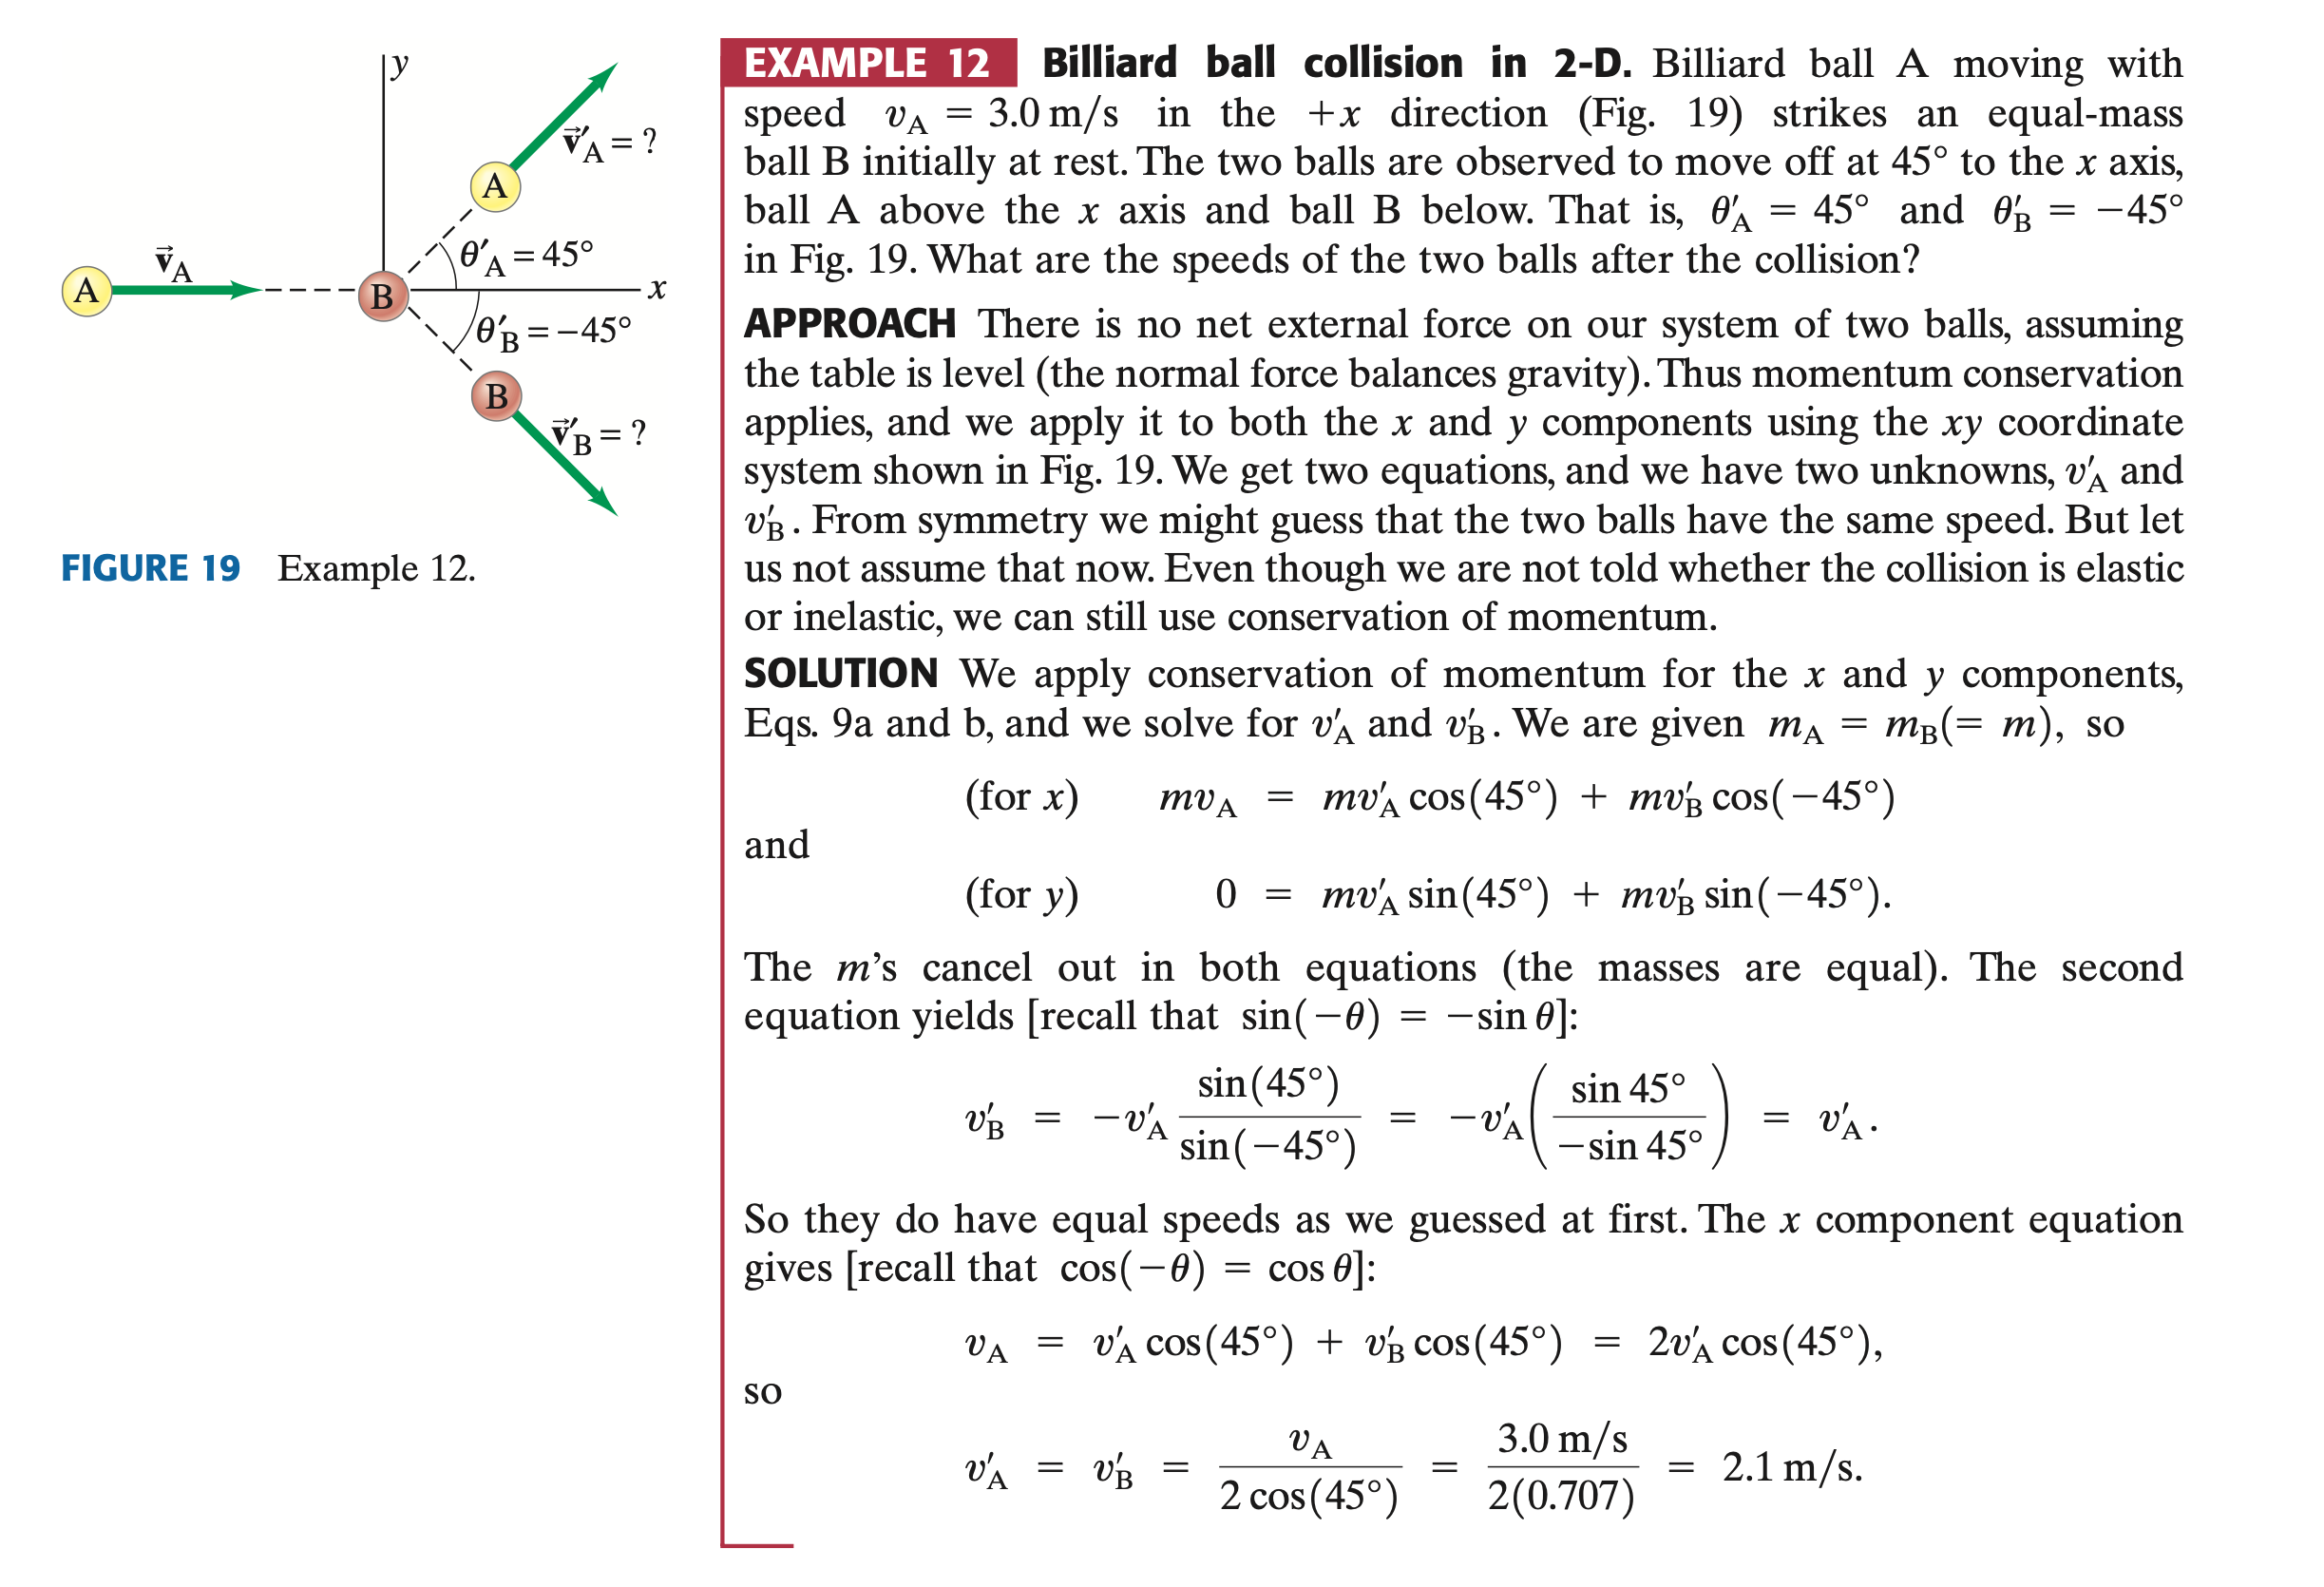
\includegraphics[scale = 0.36]{Examples/Dynamica/9.12.png}
% \end{ex}


\newpage

\section{Rotatie - Krachtmoment - Impulsmoment}

\vspace{0.5cm}

% \begin{theo}[Rotationele grootheden]{Rotationele grootheden}
%     \begin{minipage}{.56\textwidth}
%         \begin{itemize}
%             \item \textbf{Hoekverplaatsing:} $ \Delta \theta = \theta_2 - \theta_1 $
%             \item \textbf{Hoek:} $ \theta = \dfrac{\ell}{R}$  
%             \item \textbf{Hoeksnelheid:} $ (= \dfrac{\text{rad}}{s})$
%             \begin{itemize}
%                 \item \textbf{Gemiddelde:} $ \omega_{gem} = \dfrac{\Delta\theta}{\Delta t}$
%                 \item \textbf{Ogenblikkelijke:} $ \omega = \lim_{\Delta t \to 0} \dfrac{\Delta\theta}{\Delta t} = \dfrac{d\theta}{dt} $ 
%             \end{itemize}
%             \item \textbf{Hoekversnelling:} $ (= \dfrac{\text{rad}}{s^2}) $
%             \begin{itemize}
%                 \item \textbf{Gemiddelde:} $ \alpha_{gem} = \dfrac{\Delta\omega}{\Delta t}$
%                 \item \textbf{Ogenblikkelijke:} $ \alpha = \lim_{\Delta t \to 0} \dfrac{\Delta\omega}{\Delta t} = \dfrac{d\omega}{dt} $ 
%             \end{itemize}
%         \end{itemize}
%     \end{minipage} 
%     \begin{minipage}{.40\textwidth}
%         \centering
%         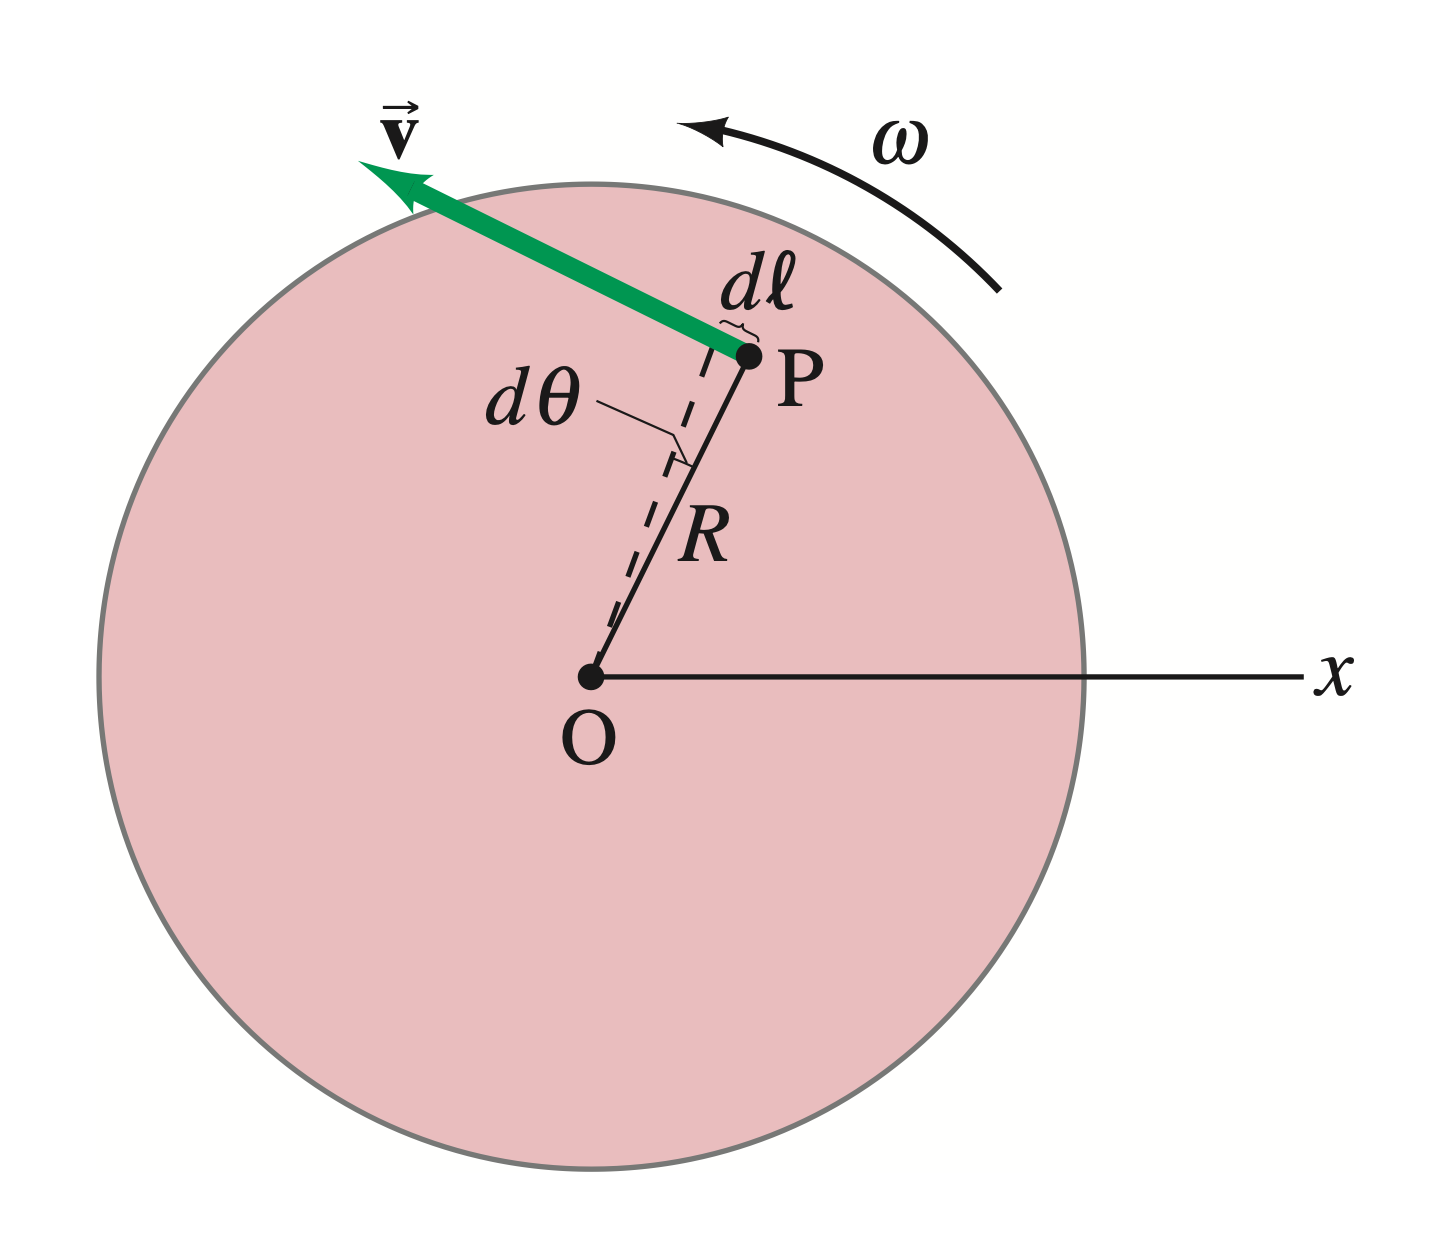
\includegraphics[scale = 0.225]{Images/Dynamica/RotatieCirkel.png}
%     \end{minipage}
% \end{theo}    

\begin{app}[Constante rotationele vs translationele versnelling]{Constante rotationele vs translationele versnelling}
    \vspace{-0.2cm}
    \begin{center}
        \def\arraystretch{2}
        \begin{tabular}{c|c}
            Rotationele beweging met constante $ \alpha $ & Translationele beweging  met constante $ a $ \\ \hline
            $ \omega = \omega_0 + \alpha t $ & $ v = v_0 +at $\\
            $ \theta = \omega_0t + \tfrac{1}{2}\alpha t^2 $ & $ x = v_0t + \tfrac{1}{2}at^2 $ \\
            $ \omega^2 = \omega_0^2 + 2\alpha\theta $ & $ v^2 = v_0^2 + 2ax $\\
            $ \omega_{gem} = \dfrac{\omega + \omega_0}{2}$ & $ v_{gem} = \dfrac{v+v_0}{2} $
        \end{tabular}
    \end{center}
\end{app}
 
\begin{theo}[Krachtmoment]{Krachtmoment}
    Het draaieffect (de hoekversnelling) van een kracht wordt bepaald door de grootte van de kracht, de richting/zin van de kracht en de "\textbf{momentarm}": afstand tussen het aangrijpingspunt van de kracht en de rotatie-as. Het \textbf{krachtmoment} is het rotationele equivalent van het translationele kracht, in formulevorm:

    \begin{equation*}
        \Vec{\tau} = \Vec{r} \times \Vec{F}
    \end{equation*}

    \noindent De grootte van het krachtmoment wordt gegeven door de volgende formule:

    \begin{equation*}
       \tau = rF\sin(\theta) = r(ma)\sin(\theta) = (m(rsin(\theta))^2)\alpha = I\alpha
    \end{equation*}

    % \noindent Sinds enkel de transversale component, de krachten, rotatie veroorzaken kunnen we de 2de wet van Newton toepassen, we vinden:

    % \begin{equation*}
    %     \tau_{net} = \sum_i \tau_i = I\alpha
    % \end{equation*}
\end{theo}

\begin{app}[Arbeid en Vermogen bij rotatie]{Arbeid en Vermogen bij rotatie}
    \begin{minipage}{.66\textwidth}
            De arbeid vericht door een object dat roteert rond een vaste as kan geschreven kan geschreven worden tegenover rotationele grootheden:
            \begin{equation*}
                W = \int \Vec{F} \cdot d\Vec{\ell} = \int F_{\perp}rd\theta
            \end{equation*}
            waarbij $ d\Vec{\ell} $ een infinitesimale afstand is loodrecht op $ r $ met grootte $ dl = rd\theta $. We weten van hierboven natuurlijk dat $ \tau = F_{\perp}r $, dus de formule wordt:
            \begin{equation*}
                W = \int_{\theta_1}^{\theta_2}\tau d\theta
            \end{equation*}
            Het vermogen bij rotatie kunnen we nu ook afleiden:
            \begin{equation*}
                P = \dfrac{dW}{dt} = \tau \dfrac{d\theta}{dt} = \tau \omega
            \end{equation*}
        \end{minipage} 
        \begin{minipage}{.33\textwidth}
            \centering
            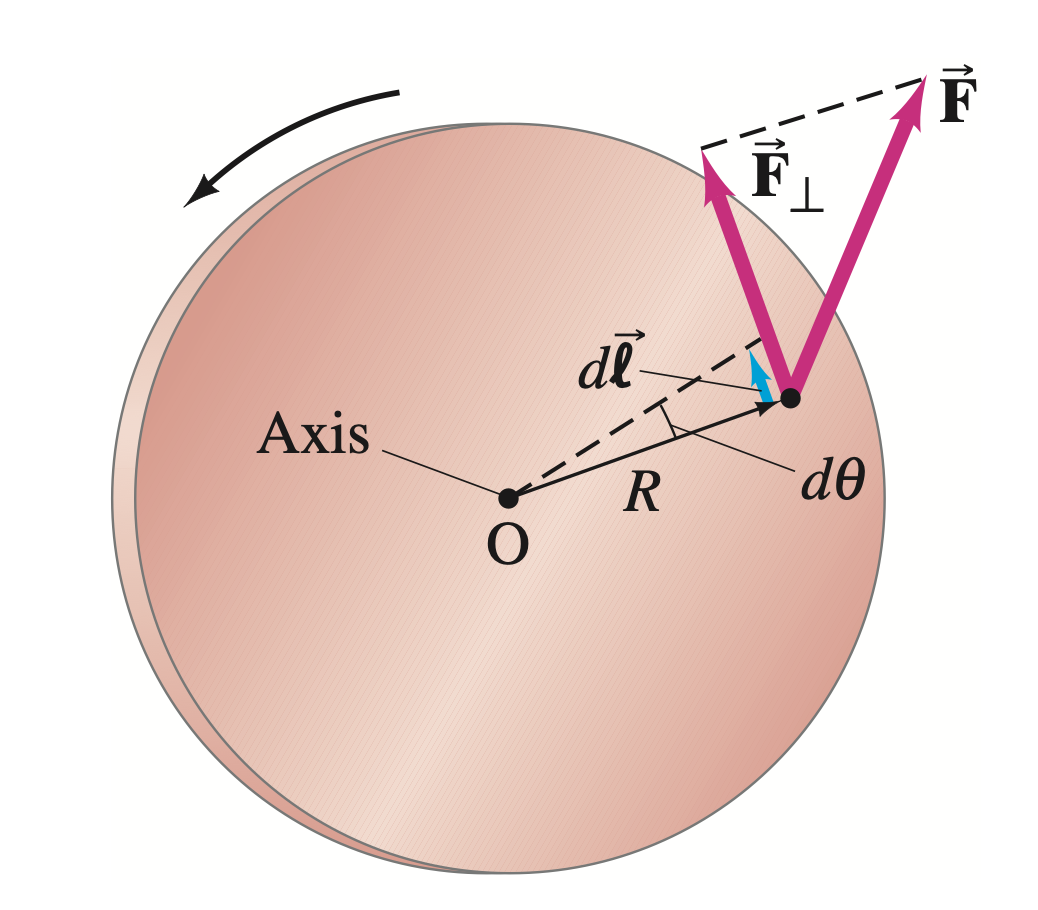
\includegraphics[scale = 0.25]{Images/Dynamica/ArbeidBijRotatie.png}
        \end{minipage}
\end{app}

\newpage

\begin{app}[Kinetische energie bij rotatie]{Kinetische energie bij rotatie}
    \vspace{-0.5cm}
    \begin{minipage}{.69\textwidth}
        Beschouw een stijf, roterend voorwerp als opgebouwd uit vele kleine deeltjes, elk met een massa $m_i$. De totale kinetische energie van het hele object is de som van de kinetische energie van alle deeltjes:
        \begin{equation*}
            K = \sum(\dfrac{1}{2}m_iv_i^2) = \sum(\dfrac{1}{2}m_ir_i^2\omega^2) =  \dfrac{1}{2}I\omega^2
        \end{equation*}
    \end{minipage} 
    \begin{minipage}{.27\textwidth}
        \centering
        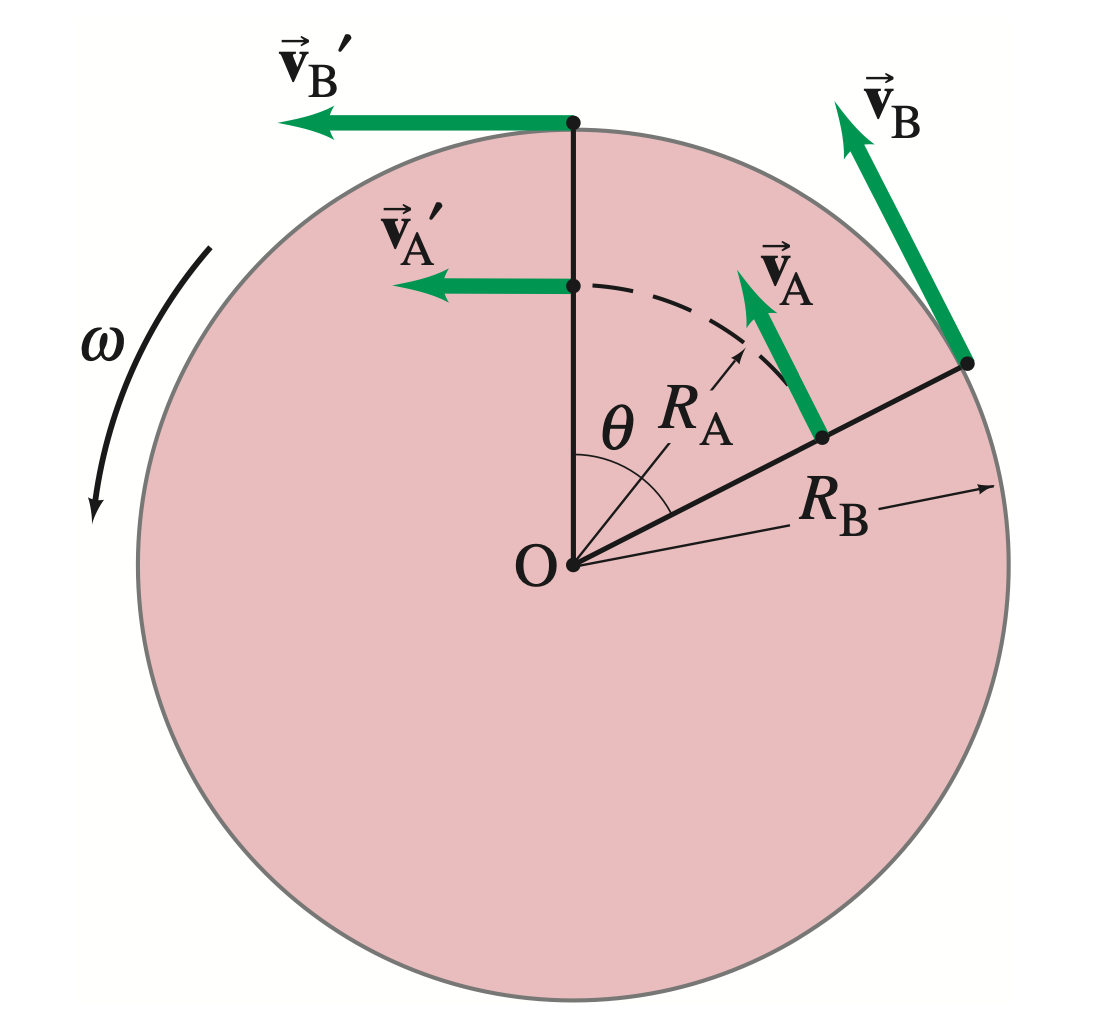
\includegraphics[scale = 0.15]{Images/Dynamica/SnelhedenOpRotatie.png}
    \end{minipage}
\end{app}

\begin{theo}[Impulsmoment]{Impulsmoment}
     Het \textbf{Impulsmoment} is de rotationele variant van het translatonele impuls, net zoals krachtmoment rotationele variant is van de translationele kracht. Het wordt gegeven door de volgende formule:
    
     \begin{equation*}
         \Vec{L} = \Vec{r} \times \Vec{p}
     \end{equation*}

     \noindent De grootte van het impulsmoment kunnen we als volgt berekenen:
     \begin{equation*}
         L = prsin(\theta) = mvrsin(\theta) = (m(rsin(\theta))^2)\omega = I\omega
     \end{equation*}
     \vspace{-0.5cm}
\end{theo}

\begin{lem}[Behoud van impulsmoment]{Behoud van impulsmoment}
    De wet van de behoud van impulsmoment stelt dat de \textbf{totale impulsmoment} ($ \Vec{L}_{net} $) van een geïsoleerd stelsel van deeltjes constant is wanneer: 
    \begin{equation*}
         \tau_{net} = \sum \tau_{ext} = \sum \dfrac{I\omega}{dt} = \dfrac{dL_{net}}{dt} = 0
    \end{equation*} 
    \vspace{-0.5cm}
\end{lem}

\begin{app}[Vergelijking: impuls – impulsmoment]{Vergelijking: impuls – impulsmoment}
    \begin{minipage}{.48\textwidth}
        \begin{center}
            
            \underline{Algemeen}: \\
            \vspace{0.25cm}
            \def\arraystretch{2.5}
            \begin{tabular}{c|c}
                impuls & impulsmoment \\ \hline
                $ \Vec{p} $ & $ \Vec{L} = \Vec{r} \times \Vec{p} $ \\ 
                $ \Vec{F} = \dfrac{d\Vec{p}}{dt} $ &  $ \Vec{\tau} = \dfrac{d\Vec{L}}{dt} $
            \end{tabular}
    
        \end{center}
    \end{minipage} 
    \begin{minipage}{.48\textwidth}
        \begin{center}
                
            \underline{Enkel bij een geïsoleerd systeem}: \\
            \vspace{0.25cm}
            \def\arraystretch{2.5}
            \begin{tabular}{c|c}
                impuls & impulsmoment \\ \hline
                behoud van impuls & behoud van impulsmoment \\ 
                $ F_{net} = \sum F_{ext} = 0 $ & $ \tau_{net} = \sum \tau_{ext} = 0 $
            \end{tabular}
        
        \end{center}
    \end{minipage}
\end{app}

% \begin{app}[Verband tussen impulsmoment en krachtmoment]{Verband tussen impulsmoment en krachtmoment}

%     Net zoals kracht zorgt voor de verandering van impuls van een voorwerp, zorgt krachtmoment voor de verandering van impulsmoment van een voorwerp: dit is het voornaamste verband.
    
%     Als we de tweede wet van newton bekijken bij rotatie, dan krijgen we de volgende formule die het verband aantoont:
    
%     \begin{equation*}
%         \sum \Vec{\tau} = I\Vec{\alpha} = I(\dfrac{d\Vec{\omega}}{dt}) = \dfrac{d(I\Vec{\omega})}{dt} = \dfrac{d\Vec{L}}{dt}
%     \end{equation*}

%     \noindent Omgekeerd kan ook als we een \textbf{puntmassa} bekijken:
%     \begin{equation*}
%         \dfrac{d\Vec{L}}{dt} = \dfrac{d(\Vec{r} \times \Vec{p})}{dt} = \dfrac{d\Vec{r}}{dt} \times \Vec{p} + \Vec{r} \times \dfrac{d\Vec{p}}{dt} = \Vec{v} \times \Vec{p} + \Vec{r} \times \Vec{F}
%     \end{equation*}
%     \noindent Het eerste lid van de som, namelijk $ \Vec{v} \times \Vec{p} $, wordt simpelweg 0, want $ \Vec{p} = m\Vec{v} $ is een lineaire combinatie van $ \Vec{v} $. Nu hebben we:
%     \begin{equation*}
%         \dfrac{d\Vec{L}}{dt} = \Vec{r} \times \Vec{F} = \tau \Rightarrow \dfrac{d\Vec{L}_{net}}{dt} = \Vec{r} \times \sum \Vec{F} = \sum \tau
%     \end{equation*}
%     % \noindent Als we nu $ \sum \Vec{F} $ pakken als de netto kracht, dan is bij een inertiaalreferentiestelsel:
%     % \begin{equation*}
%     %    \dfrac{d\Vec{L}}{dt} = \Vec{r} \times \sum \Vec{F} = \sum \Vec{\tau}
%     % \end{equation*}
%     \vspace{-0.5cm}
% \end{app}





\newpage

% \section{Impulsmoment}

% \vspace{0.5cm}

% \begin{theo}[Impulsmoment]{Impulsmoment}
     Het \textbf{Impulsmoment} is de rotationele variant van het translatonele impuls, net zoals krachtmoment rotationele variant is van de translationele kracht. Het wordt gegeven door de volgende formule:
    
     \begin{equation*}
         \Vec{L} = \Vec{r} \times \Vec{p}
     \end{equation*}

     \noindent De grootte van het impulsmoment kunnen we als volgt berekenen:
     \begin{equation*}
         L = prsin(\phi) = mvrsin(\phi) = m(\omega r)rsin(\phi) = I\omega
     \end{equation*}
     \vspace{-0.5cm}
\end{theo}

\begin{app}[Verband tussen impulsmoment en krachtmoment]{Verband tussen impulsmoment en krachtmoment}

    Net zoals kracht zorgt voor de verandering van impuls van een voorwerp, zorgt krachtmoment voor de verandering van impulsmoments van een voorwerp: dit is het voornaamste verband. Als we de tweede wet van newton bekijken bij rotatie, dan krijgen we de volgende formule die het verband aantoont:
    
    \begin{equation*}
        \sum \Vec{\tau} = I\Vec{\alpha} = I(\dfrac{d\Vec{\omega}}{dt}) = \dfrac{d(I\Vec{\omega})}{dt} = \dfrac{d\Vec{L}}{dt}
    \end{equation*}

    \noindent Omgekeerd kan ook als we een \textbf{puntmassa} bekijken:
    \begin{equation*}
        \dfrac{d\Vec{L}}{dt} = \dfrac{d(\Vec{r} \times \Vec{p})}{dt} = \dfrac{d\Vec{r}}{dt} \times \Vec{p} + \Vec{r} \times \dfrac{d\Vec{p}}{dt} = \Vec{v} \times \Vec{p} + \Vec{r} \times \Vec{F}
    \end{equation*}
    \noindent Het eerste lid van de som, namelijk $ \Vec{v} \times \Vec{p} $, wordt simpelweg 0, $ \Vec{v} $ is een lineaire combinatie van $ \Vec{p} $. Nu hebben we:
    \begin{equation*}
        \dfrac{d\Vec{L}}{dt} = \Vec{r} \times \Vec{F}
    \end{equation*}
    \noindent Als we nu $ \sum \Vec{F} $ pakken als de netto kracht, dan is bij een inertiaalreferentiestelsel:
    \begin{equation*}
       \dfrac{d\Vec{L}}{dt} = \Vec{r} \times \sum \Vec{F} = \sum \tau
    \end{equation*}
    \vspace{-0.5cm}
\end{app}

\begin{app}[Vergelijking: impuls – impulsmoment]{Vergelijking: impuls – impulsmoment}
    \begin{minipage}{.4\textwidth}
        \begin{center}
            
            \underline{Algemeen}: \\
            \vspace{0.25cm}
            \def\arraystretch{2.5}
            \begin{tabular}{c|c}
                impuls & impulsmoment \\ \hline
                $ \Vec{p} $ & $ \Vec{L} = \Vec{r} \times \Vec{p} $ \\ 
                $ \Vec{F} = \dfrac{d\Vec{p}}{dt} $ &  $ \Vec{\tau} = \dfrac{d\Vec{L}}{dt} $
            \end{tabular}
    
        \end{center}
    \end{minipage} 
    \begin{minipage}{.6\textwidth}
        \begin{center}
                
            \underline{Enkel bij een geïsoleerd systeem}: \\
            \vspace{0.25cm}
            \def\arraystretch{2.5}
            \begin{tabular}{c|c}
                impuls & impulsmoment \\ \hline
                behoud van impuls & behoud van impulsmoment \\ 
                $ F_{net} = \sum \Vec{F}_{ext} = 0 $ & $ \tau_{net} = \sum \Vec{\tau}_{ext} = 0 $
            \end{tabular}
        
        \end{center}
    \end{minipage}
\end{app}



% \newpage

\vspace*{\fill}
\begin{center}
    
\section*{Elektriciteit}
\end{center}

\vspace*{\fill}

\newpage

\section{Elektrische velden}

\vspace{0.5cm}

\begin{theo}[Elektrische ladingen]{Elektrische ladingen}
    \begin{itemize}
        \item tegengestelde ladingen trekken elkaar aan en gelijke ladingen stoten elkaar af
        \item gekwantificeerde grootheid, geen fracties
    \end{itemize}
\end{theo}

\begin{lem}[Behoud van totale lading]{Behoud van totale lading}
    Bij een geïsoleerd systeem blijft de totale aantal lading gelijk, er is enkel \textbf{transfert} van lading
\end{lem}

\begin{app}[Elektrische lading in het atoom – isolator $ \leftrightarrow $ geleider]{Elektrische lading in het atoom  isolator geleider}

    \begin{itemize}
        \item \textbf{Geleider:} \underline{sommige} elektronen zijn ongebonden en kunnen vrij bewegen
        \item \textbf{Isolator:} \underline{alle} elektronen zijn gebonden en onbeweeglijk
        \item \textbf{Halfgeleider:} ergens tussenin
    \end{itemize}

\end{app}

\begin{theo}[Coulombkracht]{Coulombkracht}

    Coulomb concludeerde dat de kracht die een klein geladen voorwerp uitoefent op een tweede evenredig is met het product van de magnitude van de lading op de ene, $ q_1 $, maal de magnitude van de lading op de andere, $ q_2 $, en omgekeerd evenredig met het kwadraat van de afstand $ r $ tussen beide. In formulevorm wordt dit:
    
    \begin{equation*}
        \hspace{3cm} \Vec{F}_{e} = k_e\dfrac{q_1q_2}{r^2}\hat{r} \quad \quad \left(\text{met} \ k_e = \dfrac{1} {4\pi\epsilon_0}\right)
    \end{equation*}
    
    % \noindent In de bovenstaande formule komen wat nieuwe letters aan bod, namelijk $ k_e $ en $ \epsilon_0 $. Het eerste kent men als de \textbf{Coulomb constante}, het tweede als de \textbf{permitiviteit} van het vacuum. \\
    
    % \noindent Bij meerdere coulombkrachten kunnen we het principe van superpositie toepassen:
    %     \begin{itemize}
    %         \item \textbf{Discreet:} $ \Vec{F}_{e^*} = k_e q^* \sum_i \dfrac{q_i}{r_i^2}\hat{r}_i$
    %         \item \textbf{Continu:} $ \Vec{F}_{e^*} = k_e q^* \int \dfrac{1}{r^2}\hat{r} dq$
    %     \end{itemize}
    % \noindent We zien ook een duidelijk verband met de zwaartekracht: vervang het concept van lading door het concept van massa en je komt de gravitatiekracht uit. Hetzelfde geldt voor het latere concept van een elektrisch veld met het gravitatieveld. \\

    \noindent \textbf{Opmerking:} de lading bij de coulombkracht is telkens de absolute waarde, omdat de grootte van een vector niet negatief mag zijn. De richting wordt dus bepaald door $\hat{r}$.
\end{theo}

\begin{theo}[Elektrisch veld]{Elektrisch veld}

    De elektrische veld vector $ \Vec{E} $ in een punt in de ruimte is gelijk aan de elektrische kracht $ \Vec{F_e} $ die op een \textbf{positieve} testlading werkt, gedeeld door de testlading. In formulevorm:
    
    \begin{equation*}
        \Vec{E} = \dfrac{\Vec{F_e}}{q} =  k_e\dfrac{q}{r^2}\hat{r}
    \end{equation*}
    
    % \noindent We vinden nu dus ook de volgende interessante formules als we spreken over een punt tegenover een puntlading:
    
    % \begin{align}
    %     \hspace{3.5cm}\Vec{F_e} &= \Vec{E}q \\
    %     \Vec{E} &= k_e\dfrac{q}{r^2}\hat{r} \quad \quad (\Vec{F}_{e} = k_e\dfrac{q_1q_2}{r^2}\hat{r})
    % \end{align}
    
    % \noindent Formules (1) en (2) kunnen we ook gebruiken als we spreken over meerdere puntladingen door opnieuw het principe van superpositie te gebruiken.

\end{theo}

\newpage

\begin{app}[Beweging van een lading in een uniform elektrisch veld]{Beweging van een lading in een uniform elektrisch veld}
    \begin{minipage}{.7 \textwidth}
        \vspace{-0.15cm}
        We vinden door de tweede wet van Newton toe te passen:
        \begin{align*}
            \Vec{F}_{net} &= \sum \Vec{F} = m\Vec{a} \\
                          &= \Vec{F_e} = q\Vec{E} = m\Vec{a}
        \end{align*}
        \noindent Hieruit volgt dus de vectoriële formule voor de versnelling veroorzaakt door een uniform elektrisch veld, namelijk:
        \begin{equation*}
            \Vec{a} = \dfrac{q}{m}\Vec{E}
        \end{equation*}
        Sinds dat de massa, het elektrisch veld en de lading constant is, blijft dus de versnelling \textbf{ook constant}! We kunnen dus de veelbesproken identiteiten hiervoor gebruiken.
    \end{minipage} 
    \begin{minipage}{.30\textwidth}
        \vspace{-0.3cm}
        \centering
        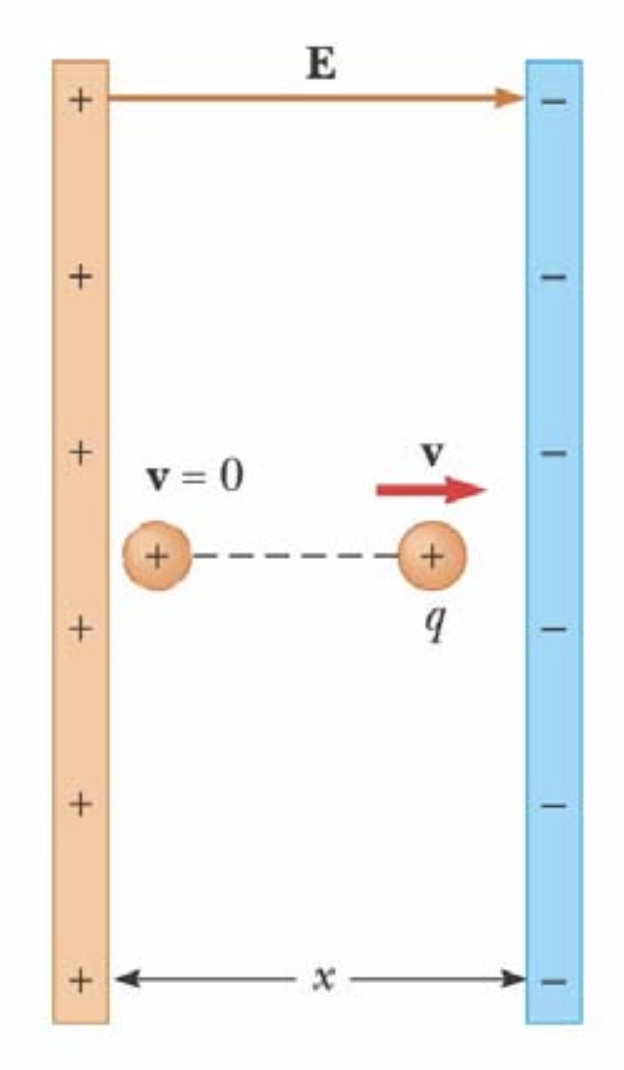
\includegraphics[scale = 0.3]{Images/Elektriciteit/UniformE.png}
    \end{minipage}

\end{app}

\begin{pro}[Geleiders in elektrostatisch evenwicht]{Geleiders in elektrostatisch evenwicht}
    \begin{itemize}
        \item Het elektrisch veld in een geleider is nul (bij elektrostatisch evenwicht mag er geen \textbf{netto} ladingsbeweging zijn)
        \item De lading van een geïsoleerde geleider bevindt zich aan het oppervlak
        \item Het elektrisch veld net buiten de geleider is loodrecht op het oppervlak en $|E| = \tfrac{\sigma}{\epsilon_0}$
        \item Oppervlakteladingsdichtheid $\sigma$ is het grootst bij de grootste oppervlaktekromming
    \end{itemize}
\end{pro}

\begin{app}[Elektrisch veld berekeningen voor continue ladingsverdelingen]{Elektrisch veld berekeningen voor continue ladingsverdelingen}

    We kunnen bij continue ladingen een infinitesimaal gebied bekijken, hier dus een infinitesimale lading en krijgen we de volgende formule:
    
    \begin{equation}
        d\Vec{E} = k_e \dfrac{dq}{r^2}\hat{r}
    \end{equation}
    
    \noindent We willen nu het totale veld bereken door te sommen over al deze infinitesimalen:
    
    \begin{equation}
        \Vec{E} = \int d\Vec{E}
    \end{equation}
    
    \noindent Als we nu een \textbf{uniforme ladingsdichtheid} definiëren, dan kunnen we meeste berekeningen oplossen omtrent continue ladings verdelingen. We definiëren:

    % \begin{equation*}
    %     dq = \rho dV = \sigma dA = \lambda dL
    % \end{equation*}
    
    \begin{itemize}
        \item \textbf{Volume-ladingsverdeling:} $ \rho = \dfrac{dq}{dV} $
        \item \textbf{Oppervlakte-ladingsverdeling:} $ \sigma = \dfrac{dq}{dA} $
        \item \textbf{Lineaire-ladingsverdeling:} $ \lambda = \dfrac{dq}{dL} $
    \end{itemize}

    \vspace{-0.3cm}
    
\end{app}

\newpage

\begin{theo}[Elektrische dipool en het dipoolmoment]{Elektrische dipool en het dipoolmoment}

    Wanneer er 2 gelijke ladingen zijn met tegengesteld teken, dus: $ +q $ en $ -q $, en ze gescheiden zijn door een lengte $ \ell $, dan kunnen we spreken over een \textbf{elektrisch dipool}. \\
    \begin{center}
       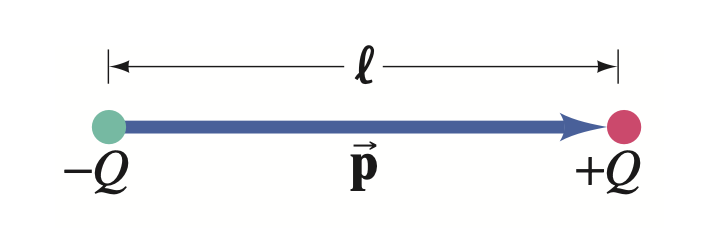
\includegraphics[scale = 0.4]{Images/Elektriciteit/Dipool.png} 
    \end{center}
    Het elektrisch dipoolmoment $ \vec{p} $ is een maat van polariteit van een binding en kan als volgt vectorieel weergegeven worden: 
    
    \begin{equation*}
        \Vec{p} = q\Vec{\ell}
    \end{equation*}
\end{theo}

\begin{app}[Dipool in een uniform veld]{Dipool in een uniform veld}
    
    \begin{minipage}{.48\textwidth}
        \begin{itemize}
            \item \textbf{Totale kracht:}
                \begin{equation*}
                    \vspace{0.25cm}
                    \Vec{F} = \Vec{F}_++\Vec{F}_- = q\Vec{E} - q\Vec{E} = 0
                \end{equation*}
            \item \textbf{Krachtmoment rond middelpunt:}
                \begin{align*}
                     \tau &= qE\dfrac{\ell}{2}\sin(\theta) - (-qE\dfrac{\ell}{2}\sin(\theta)) \\
                     &= qE\dfrac{\ell}{2}\sin(\theta) + qE\dfrac{\ell}{2}\sin(\theta)  \\
                     &= pE\sin(\theta)  \\
                     \Vec{\tau} &= \Vec{p} \times \Vec{E}
                \end{align*}
            \item \textbf{Arbeid:}
        \end{itemize}
    \end{minipage} 
    \begin{minipage}{.48\textwidth}
        \centering
        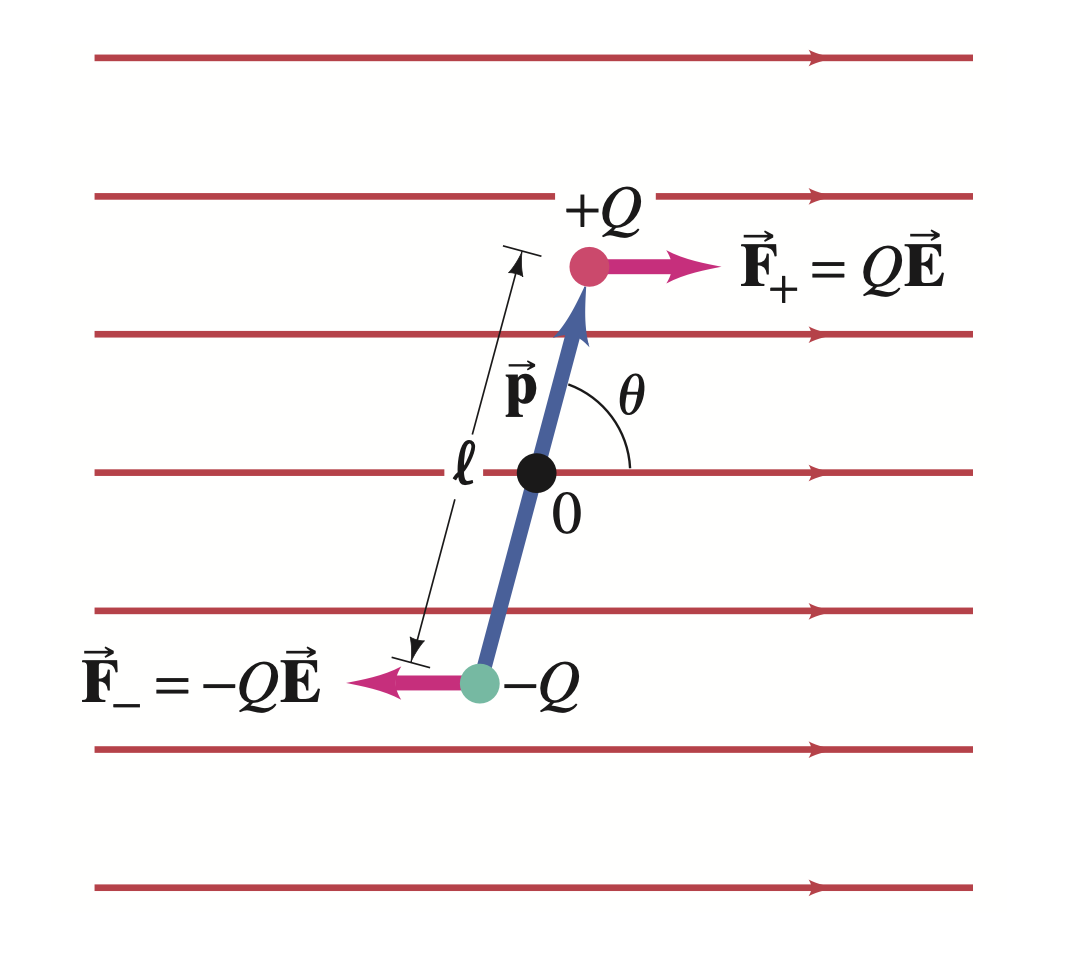
\includegraphics[scale = 0.35]{Images/Elektriciteit/UniformDipool.png}
    \end{minipage}
    
    \begin{minipage}{.5\textwidth}
            \begin{align*}
                \hspace{1.1cm}
                W &= \int_{\theta_1}^{\theta_2} \tau d\theta \\ 
                  &= \textbf{-}pE\int_{\theta_1}^{\theta_2} \sin(\theta) d\theta \quad \quad (\text{$d\theta$ is negatief dus, - voor positieve $W$}) \\
                  &= pE(\cos(\theta_{2})-\cos(\theta_{1})) \\
                  &= -\Delta U \\ 
                U &= -\Vec{p} \cdot \Vec{E} \quad \quad (inertiaalstelsel: \theta_1 = \dfrac{\pi}{2}) \\\\
           \end{align*}
    \end{minipage} 
    \begin{minipage}{.5\textwidth}
    \end{minipage}
    \vspace{-1cm}
\end{app}

\newpage

\section{De wet van Gauss}

\vspace{0.5cm}

\begin{theo}[Elektrische flux]{Elektrische flux}

    % Het concept van \textbf{elektrische flux} zal heel interessant blijken, vooral omdat dit ons een nieuwe methode geeft om elektrisch velden te berekenen. 
    
    De elektrische flux doorheen een oppervlak is de oppervlakte-integraal van de elektrische veldsterkte over dat oppervlak. Laten we eerst kijken naar, zoals vaker, het makkelijker geval, namelijk wanneer we spreken over een uniform elektrisch veld:
    
    \begin{equation*}
        \Phi_E = \Vec{E}\cdot\Vec{A}
    \end{equation*}
    
    \noindent Als we spreken over een niet-uniform veld, dan spreken we eigenlijk over infinitesimale uniforme velden. De formule wordt dus:
    \begin{equation*}
        \Phi_E = \oint \Vec{E}\cdot d\Vec{A}
    \end{equation*}
    
    \noindent De nettoflux $ \Phi_e $ is recht evenredig met netto aantal veldlijnen dat het oppervlakte verlaat.
    
        \begin{center}
            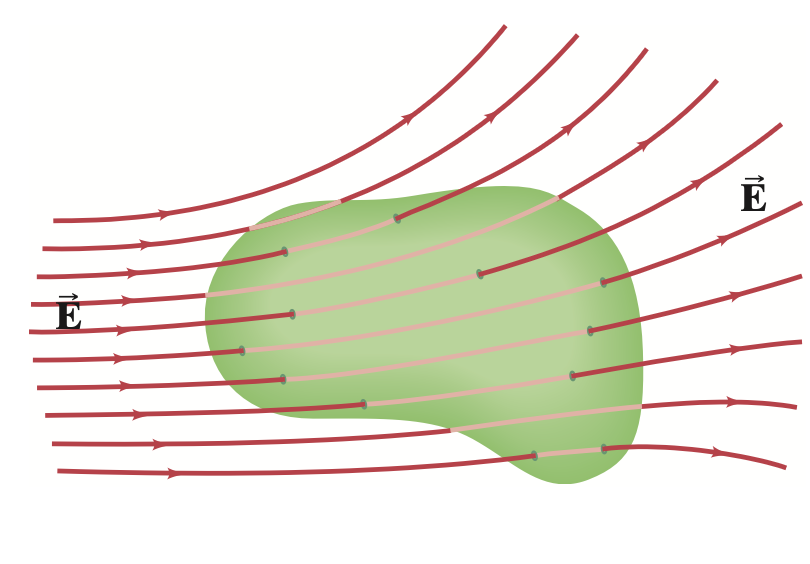
\includegraphics[scale = 0.35]{Images/Elektriciteit/OppervlakteGeenLading.png}
        \end{center}
    % Sinds er een verband is tussen elektrisch veld en gravitatieveld, kunnen we ook praten over gravitationele flux bij dynamica.
\end{theo}

\begin{lem}[Gauss voor Elektriciteit]{Gauss voor Elektriciteit}

    De wet van Gauss zegt dat de nettoflux door een willekeurig \textbf{gesloten} oppervlak dat een lading $ q $ omsluit, is steeds gelijk aan $ \tfrac{q_{in}}{\epsilon_0} $, in formulevorm:
    
    \begin{equation*}
        \Phi_E = \oint \Vec{E}\cdot d\Vec{A} = \dfrac{q_{in}}{\epsilon_0}
    \end{equation*}
    
    \noindent Hieruit volgt dus dat de nettoflux door een willekeurig gesloten oppervlak dat geen lading omsluit, is steeds gelijk aan 0. 
    % Dit kunnen we intuitief ook makkelijk begrijpen: als er een lading zou zijn, dan zouden de binnenkomende en buitengaande veldlijnen niet meer een gelijk aantal zijn en is dus de nettoflux niet nul.
\end{lem}

% \begin{app}[Wet van Gauss bij meerdere elektrische velden]{Wet van Gauss bij meerdere elektrische velden}
% We kunnen natuurlijk de formule van hierboven ook gebruiken als er meerdere elektrische velden aanwezig zijn. Dit wordt dan door de wet van de superpositie:

% \begin{equation*}
%     \Phi_e = \oint \Vec{E}_{tot}\cdot d\Vec{A} = \oint (\sum_i \Vec{E}_i) \cdot d\Vec{A}  = \dfrac{q_{in}}{\epsilon_0}
% \end{equation*}

% \end{app}

% \begin{app}[Wet van Coulomb vs wet van Gauss]{Wet van Coulomb vs wet van Gauss}
%     \begin{center}
%         \def\arraystretch{2.5}
%         \begin{tabular}{c|c}
%             wet van Coulomb & wet van Gauss \\ \hline
%             $ E = k\dfrac{Q}{r^2} $ & $ \oint \Vec{E}\cdot d\Vec{A} = 4\pi kQ$ \\ 
%             $ E = \dfrac{1}{4\pi\epsilon_0}\dfrac{Q}{r^2} $ & $ \oint \Vec{E}\cdot d\Vec{A} = \dfrac{Q_{in}}{\epsilon_0} $
%         \end{tabular}
%     \end{center}
% \end{app}

% \begin{prf}[Formeel bewijs van de wet van Gauss]{Formeel bewijs van de wet van Gauss}

%     \begin{itemize}
%         \item{Lading \emph{binnen} gesloten oppervlak}
            

%             \begin{center}
%                 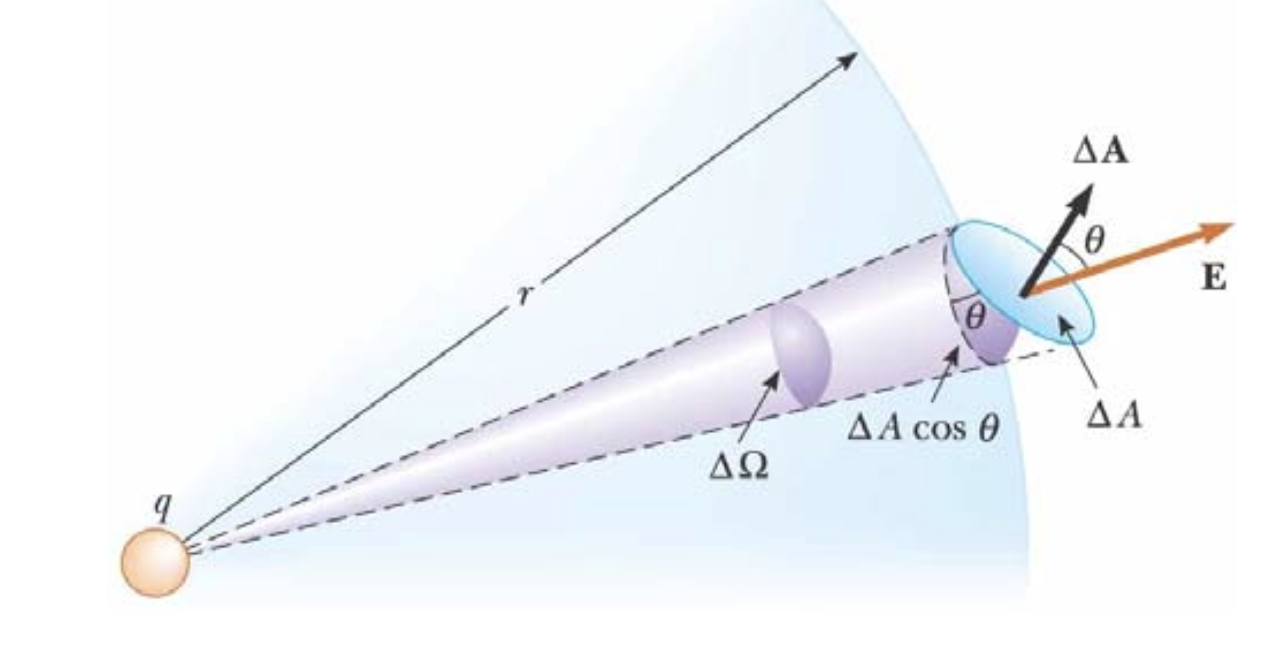
\includegraphics[scale = 0.3]{Images/Elektriciteit/Ruimtehoek.png}
%             \end{center}
        
%         \item{Lading \emph{buiten} gesloten oppervlak}
        
%             \begin{minipage}{.48\textwidth}
%             \end{minipage} 
%             \begin{minipage}{.48\textwidth}
%             \end{minipage}
    
%     \end{itemize}
% \end{prf}

% \begin{pro}[Eigenschappen van geleiders in elektrostatisch evenwicht]{Geleiders in elektrostatisch evenwicht}

%     \begin{minipage}{.55\textwidth}
%         \begin{itemize}
%             \item Elektrisch veld in de geleider is nul
%             \item De lading van een geïsoleerde geleider bevindt zich aan het oppervlak
%             \item Elektrisch veld net buiten de geleider:
%             \begin{itemize}
%                 \item $ E \perp A $
%                 \item $ E = \dfrac{\sigma}{\epsilon_0} $, want: \\
%                         $ \Phi_e = \oint \Vec{E}\cdot d\Vec{A} = EA = \dfrac{Q_{in}}{\epsilon_0} = \dfrac{\sigma A}{\epsilon_0} \Rightarrow E = \dfrac{\sigma}{\epsilon_0}$
%             \end{itemize}
%             \item Oppervlakteladingsdichtheid is grootst bij grootste oppervlaktekromming
%         \end{itemize}
%     \end{minipage} 
%     \begin{minipage}{.41\textwidth}
%         \centering
%         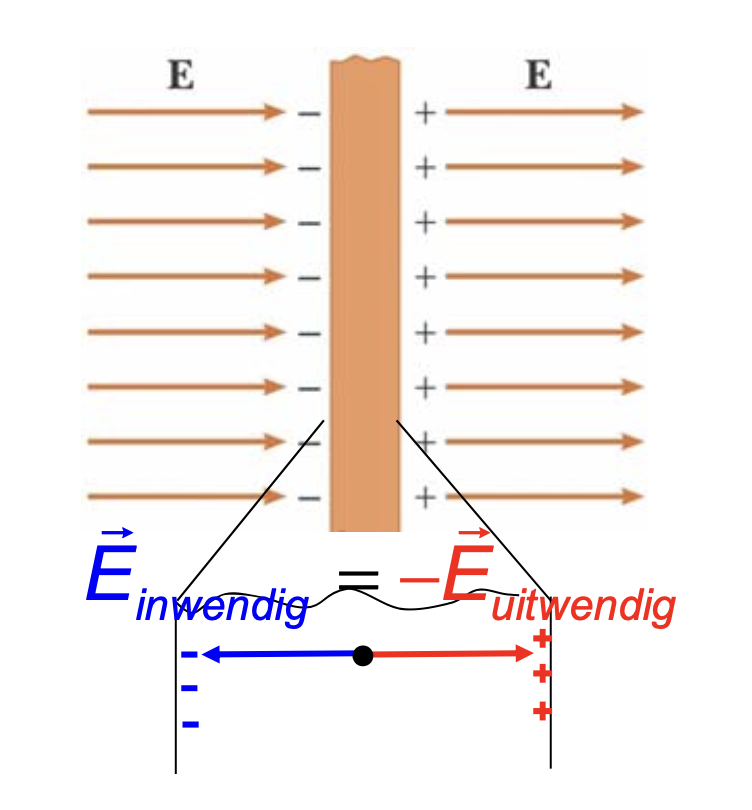
\includegraphics[scale = 0.4]{Images/Elektriciteit/Elektrisch veld in een geleider.png}
%     \end{minipage}

% \end{pro}




\newpage

\section{Elektrische potentiaal}

\vspace{0.5cm}

\begin{theo}[Elektrische potentiële energie]{Elektrische potentiële energie}

Om de wet van behoud van energie toe te mogen passen, moeten we nog \textbf{elektrische potentiële energie} definiëren. 

% We weten uit hoofdstuk 8:

% \begin{equation*}
%     \Delta U = U_b - U_a = \int_a^b dU = -\int_a^b \Vec{F} \cdot d\Vec{r} = -W
% \end{equation*}

% \noindent Dit kunnen we nu toepassen in de context van de elektrostatische kracht, vermits deze conservatief is:

\begin{equation*}
    \hspace{3.25cm}
    \Delta U = -\int_a^b \Vec{F_e} \cdot d\Vec{r} = -q \int_a^b \Vec{E} \cdot d\Vec{r} = -W \quad \quad (\text{met $q$ een testlading})
\end{equation*}

\noindent In overeenkomst met de wet van behoud van energie, wordt nu elektrische potentiele energie getransformeerd naar kinetische energie. 

\end{theo}

\begin{theo}[Elektrische potentiaal en potentiaalverschil]{Elektrische potentiaal en potentiaalverschil}

    Het \textbf{elektrische potentiaal} $ V $ is een \textbf{scalaire} grootheid die gedefinieerd wordt door het elektrische potentiële energie per lading. In formulevorm:
    
    \begin{equation*}
        V = \dfrac{U}{q}
    \end{equation*}
    
    \noindent Het maakt niet per se uit hoeveel potentiële energie een systeem heeft op een bepaald moment, maar wel hoeveel er naar kinetische energie wordt omgezet. Dus: enkel verschillen in potentiële energie zijn zinvol of betekenisvol. In formulevorm:
    
    \begin{equation*}
         \Delta V = \dfrac{\Delta U}{q} = \dfrac{-W}{q}
    \end{equation*}
    
    \noindent Dit noemt men het \textbf{potentiaalverschil}. De eenheid van eletrische potentiaal, en dus potentiaalverschil, noemt men de volt: $ V = \dfrac{J}{C} $. \\
    
    \noindent Als we de formule van de elektrische potentiele energie in functie van het potentiaalverschil schrijven, dan krijgen we:
    
    \begin{equation*}
        \Delta V  = -\dfrac{1}{q} \int_a^b \Vec{F_e} \cdot d\Vec{r} = -\int_a^b \Vec{E} \cdot d\Vec{r} 
    \end{equation*}
    
    \noindent Dit toont een belangrijk verband aan tussen het elektrische potentiaal en elektrisch veld. Als het veld uniform is, dan hebben de elektrisch veld en de verplaatsing vectoren dezelfde richting en volgt:
    \begin{equation*}
        \Delta V  = -\int_a^b \Vec{E} \cdot d\Vec{r} = - E \int_a^b dr = -Er
    \end{equation*}
    
\end{theo}

\begin{theo}[Equipotentiaaloppervlakken]{Equipotentiaaloppervlakken}

    \textbf{Equipotentiaaloppervlakken} zijn oppervlakken die punten met een equivalent potentiaal verbinden en die loodrecht staan  op de veldlijnen, want de potentiaal moet doorheen het oppervlak gelijk zijn.
    
\end{theo}

\begin{app}[Elektrische potentiaal tegenover puntladingen]{Elektrische potentiaal tegenover puntladingen}

    We hebben eerder besproken dat enkel het potentiaalverschil zinvol is. We kunnen dus een punt pakken waar het potentiaal 0 is en hiermee kunnen we het potentiaal van een singuliere puntlading berekenen. We weten ook dat het elektrisch veld door een singuliere puntlading de volgende formule heeft:
    
    \begin{equation*}
        \Vec{E} = \dfrac{\Vec{F}_e}{q_0}= k_e\dfrac{q}{r^2}\hat{r}
    \end{equation*}
    
    
    \noindent Stel nu dat $ V_b = 0 $ en $ r_b = \infty $ en we een recht pad volgen van $ a \to b $:
    
    \begin{equation*}
        V_a = - \int_a^b \Vec{E} \cdot d\Vec{r} = - E \int_a^{b} dr = - \dfrac{1}{4\pi\epsilon_0}(\dfrac{q}{r_b} - \dfrac{q}{r_a})  = \dfrac{1}{4\pi\epsilon_0}\dfrac{q}{r_a}
    \end{equation*}
    
    \noindent Het elektrische potentiaal is een \textbf{scalar}, dus we kunnen meerdere potentialen gewoon optellen zonder rekening te moeten houden met richting.
    
    \begin{equation*}
        V_{tot} = \sum_i V_{i}= k(\sum_i \dfrac{q_i}{r_{i}})
    \end{equation*}
    
    \noindent We kunnen het concept van meerdere puntladingen verbreden tot infinitesimale puntladingen als we spreken over een continue ladingsverdeling. Zoals vaker volgt nu de volgende formule:
    
    \begin{equation*}
        V = \dfrac{1}{4\pi\epsilon_0}\int\dfrac{dq}{r}
    \end{equation*}
    
    \noindent In principe geeft deze formule ook het volgende:
    
    \begin{equation*}
        dV = -\Vec{E} \cdot d\Vec{s}
    \end{equation*}
    
    \noindent \textbf{Opmerking:} het elektrisch veld in bijvoorbeeld de x-richting is dus gelijk aan $ E_x = -\dfrac{dV}{dx} $ Hieruit kunnen we de volgende formule afleiden:
    
    \begin{equation*}
        \Vec{E} = (-\nabla V)\hat{r} = -\dfrac{dV}{dx}\hat{i} -\dfrac{dV}{dy}\hat{j} -\dfrac{dV}{dz}\hat{k}
    \end{equation*}

\end{app}

\begin{app}[Elektrische potentiaal bij een dipool]{Elektrische potentiaal bij een dipool}

    \begin{minipage}{.68 \textwidth}
        \vspace{-0.4cm}
        Het elektrische potentiaal op een arbitrair punt P wordt gegeven door de volgende formule waarbij $ V = 0 \ op \ r = \infty $:
        
        \begin{equation*}
            V = k\dfrac{q}{r} + k \dfrac{(-q)}{r + \Delta r} = kq(\dfrac{1}{r} - \dfrac{1}{r+ \Delta r}) = kq\dfrac{\Delta r}{r(r+\Delta r)}
        \end{equation*}
        
        \noindent Deze vergelijking wordt vele malen eenvoudiger als we een punt P pakken veel verder weg dan de scheiding tussen de twee ladingen. We zien op de tekening dat: $ \Delta r \approx \ell\cos(\theta) $. Als we nu dus $ r \gg \ell $ pakken, dan is dus $ r \gg \Delta r $ en verandert onze formule:
        
        \begin{equation*}
            V = k\dfrac{q\ell\cos(\theta)}{r^2} = k\dfrac{p\cos(\theta)}{r^2} \quad \quad (r \gg \ell)
        \end{equation*}
        
        % Als we nu herinneren dat het dipoolmoment $ p = Q\ell $, dan krijgen we de volgende formule:
        
        % \begin{equation*}
        %     V = k\dfrac{p\cos(\theta)}{r^2} \quad \quad (r \gg \ell)
        % \end{equation*}
    
    \end{minipage} 
    \begin{minipage}{.28\textwidth}
        \vspace{-0.3cm}
        \begin{center}
            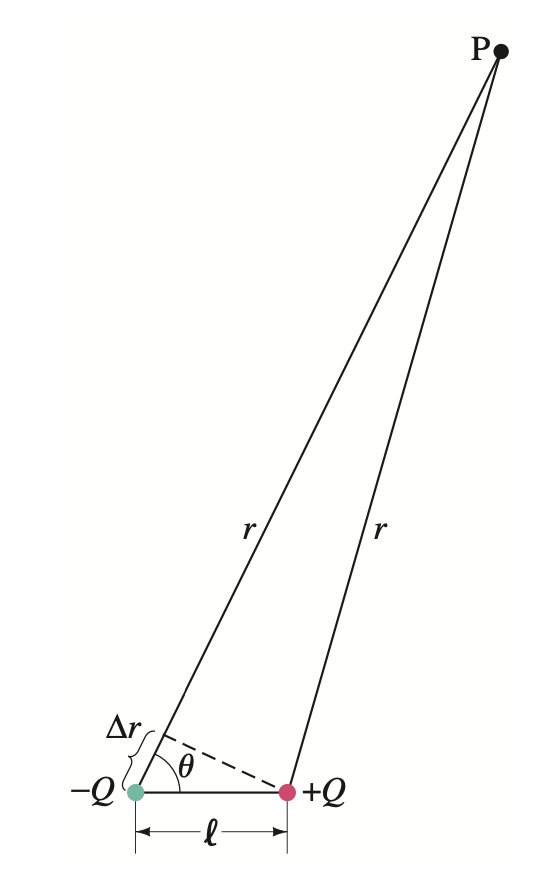
\includegraphics[scale = 0.4]{Images/Elektriciteit/DipoolPotentiaal.png}
        \end{center}
    \end{minipage}

    % \noindent De volgende tekening toont de equipotentiaaloppervlakken aan van een dipool:
    
    % \begin{center}
    %     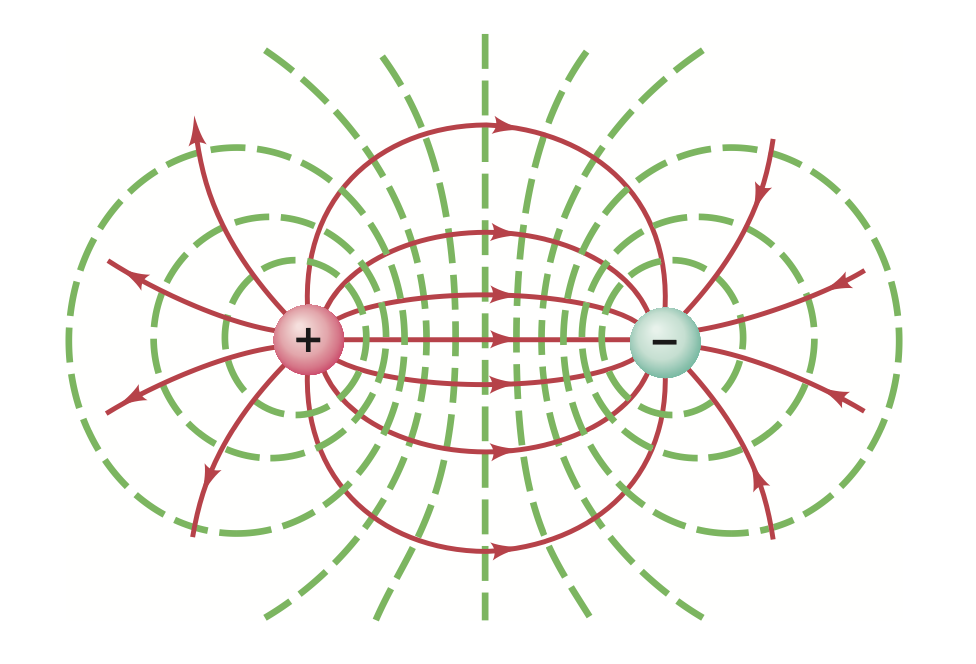
\includegraphics[scale = 0.45]{Images/Elektriciteit/DipoolEquipotentiaaloppervlakken.png}
    % \end{center}
\end{app}

\newpage

\begin{app}[Elektrische potentiaal bij een geladen geleider in evenwicht]{Elektrische potentiaal bij een geladen geleider in evenwicht}

    \begin{itemize}
        \item{\underline{Binnen de geleider zonder caviteit}:} \\
        
        We weten dat het elektrisch veld in de geleider nul is als de geleider zich in een elektrostatisch evenwicht bevindt. We berekenen nu het potentiaalverschil:
        
        \begin{equation*}
            \Delta V = \dfrac{\Delta U}{q} = - \int_a^b \Vec{E} \cdot d\Vec{\ell} = 0
        \end{equation*}
                
        \noindent We kunnen nu bepaalde uitspraken doen over het potentiaalverschil bij een geleider in elektrostatisch evenwicht:
        
        \begin{itemize}
            \item Het oppervlak van een geleider in elektrostatisch evenwicht heeft een constante potentiaal.
            \item  De potentiaal binnenin een geleider is constant, en gelijk aan de potentiaal aan het oppervlak. Er is dus \textbf{geen arbeid} vereist om een lading te bewegen binnenin een geleider
        \end{itemize}
        
        \item{\underline{Binnen de geleider met caviteit}:}
        
        \begin{minipage}{.48\textwidth}
        Het veld in een caviteit (waarbinnen zich geen lading bevindt) omgeven door een geleider is nul. Als er wel een lading in zit, dan moet er aan de rand een gelijke tegengestelde lading zijn opdat er geen elektrisch veld buiten de caviteit zou zijn. Binnenin de caviteit is er natuurlijk dan wel een elektrisch veld. Wegens de wet van behoud van lading, moet er een gelijke positieve lading op het oppervlak van de geleider zijn!
        
        \end{minipage} 
        \begin{minipage}{.48\textwidth}
            \centering
            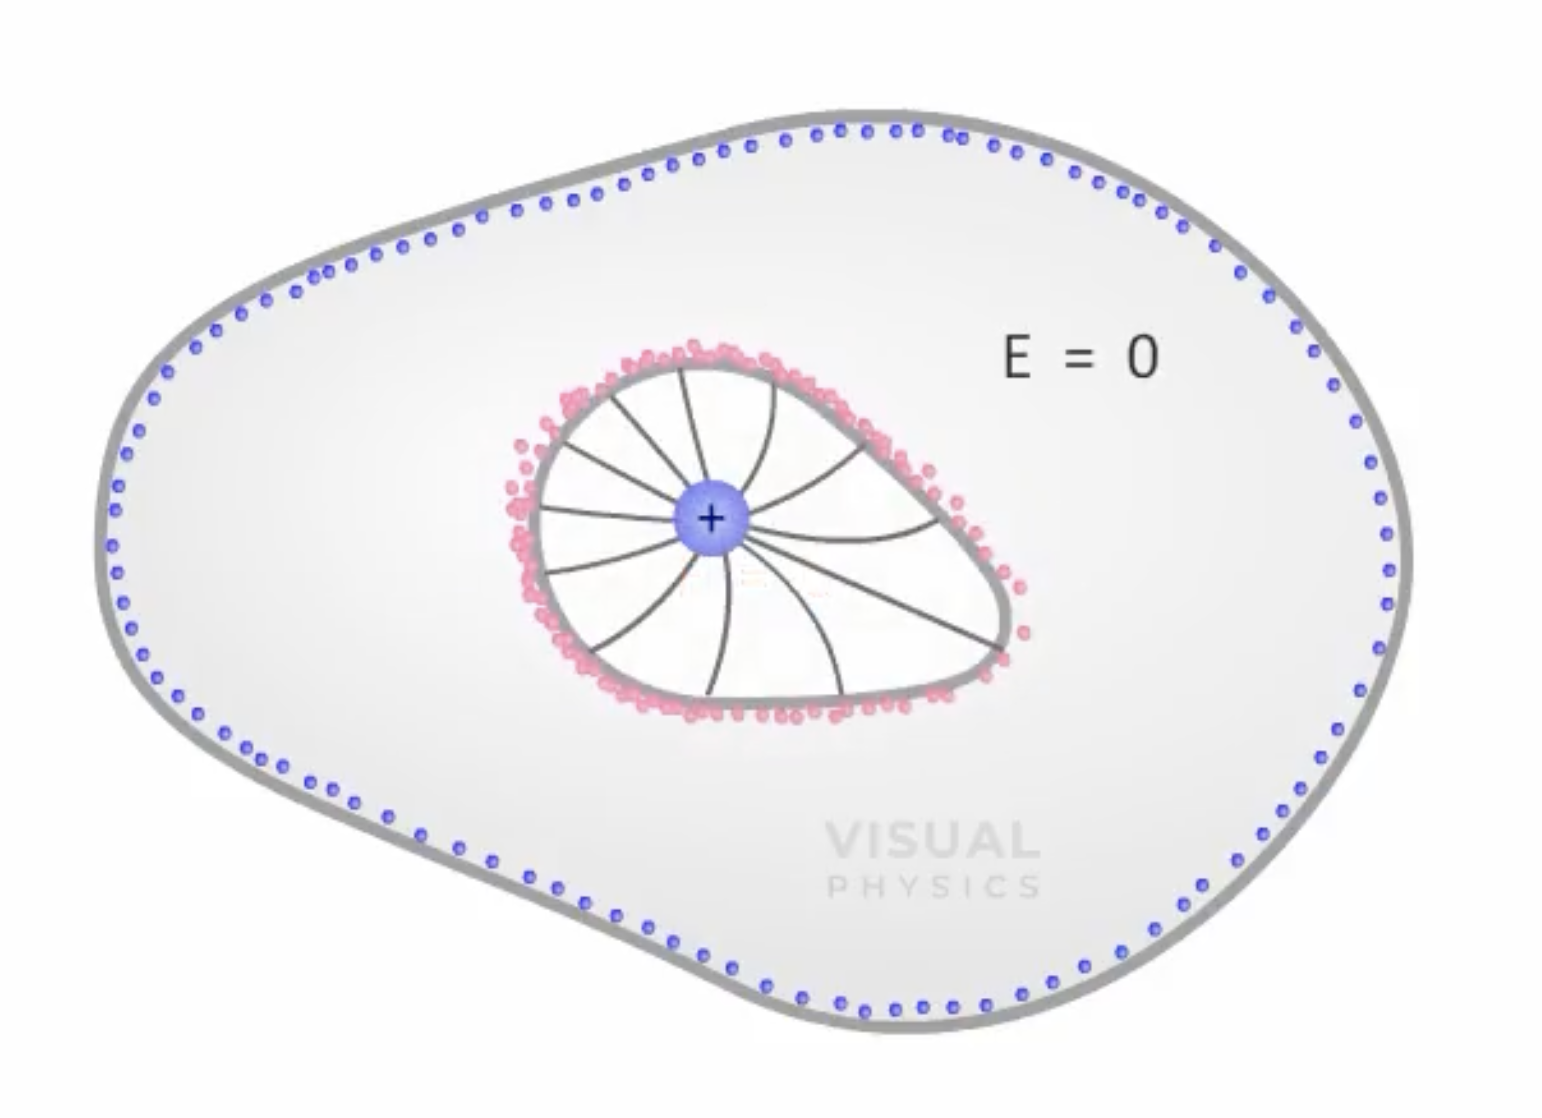
\includegraphics[scale = 0.25]{Images/Elektriciteit/Caviteit.png}
        \end{minipage}
        
        \item{\underline{Buiten de geleider}:} \\
        
        We berekenen het potentiaal van op het oppervlak van een sferische geleider om tot bepaalde conclusies te kunnen komen:
        
        \begin{equation*}
            V = k \dfrac{q}{r} = k \dfrac{\sigma A}{r} = k\dfrac{\sigma 4 \pi r^2}{r} = \dfrac{\sigma r}{\epsilon_0} = Er
        \end{equation*}
        
        \noindent Hieruit volgt dus dat het elektrisch veld groter is nabij convexe punten, vermits het recht evenredig is met de oppervlakteladingsdichtheid. In formulevorm: 
        
        \begin{equation*}
            E \sim \sigma
        \end{equation*}
    
    \end{itemize}
\end{app}



\newpage

\section{Condensatoren en diëlektrica}

\vspace{0.5cm}

\input{Chapters/Elektriciteit/Condensatoren en diëlektrica.tex}

\newpage

\newpage

\section{Elektrische stroom en weerstand}

\vspace{0.5cm}

\begin{theo}[Elektrische stroom]{Elektrische stroom}
    \textbf{Elektrische stroom} is het tempo waarmee er elektrische lading door een oppervlak stroomt. Het is dus eigenlijk een vorm van snelheid voor de lading. Voor een constant tempo bekomen we

    \begin{equation*}
        I_{gem} = \dfrac{\Delta Q}{\Delta t}
    \end{equation*} 
    
    \noindent en bij variërend tempo bekomen we

    \begin{equation*}
        I = \dfrac{dQ}{dt}
    \end{equation*} 
    De stroomzin is in de omgekeerde richting van de elektronenstroom,
    \begin{center}
        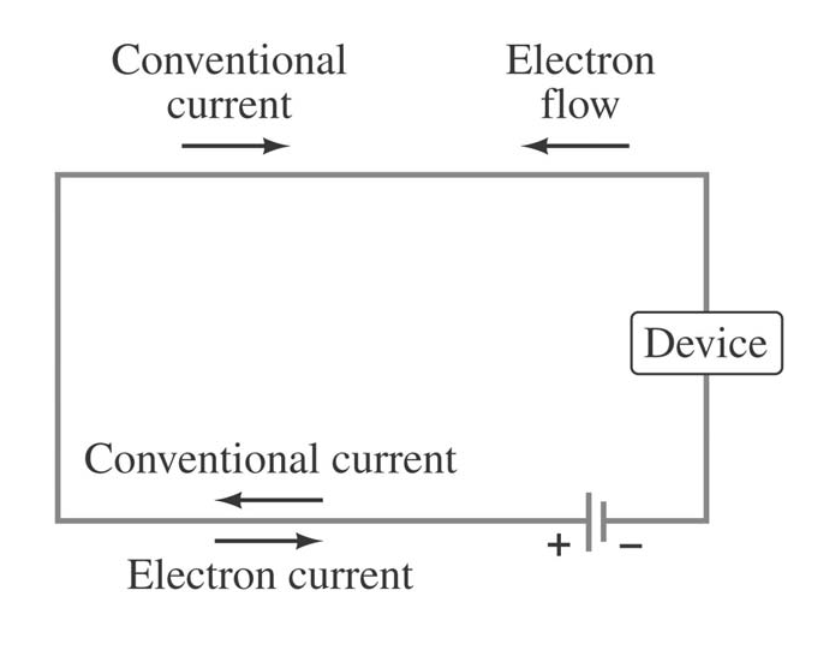
\includegraphics[scale = 0.4]{Images/Elektriciteit/Stroomzin.png}
    \end{center}
    maar wordt gedragen door de elektronen in metalen draden op microscopisch niveau en in fluïdum door protonen of elektronen. De stroomzin is dus eerder een conventie.
\end{theo}

\begin{app}[Microscopisch model van elektrische stroom]{Microscopisch model van elektrische stroom}
    We nemen aan dat we ons niet in het electrostatisch geval bevinden, namelijk dat
    \begin{equation*}
        \Vec{E} \neq 0
    \end{equation*}
    en dus de ladingen vrij zijn om te bewegen. We definiëren nu een nieuwe microscopische grootheid, de stroomdichtheid $\Vec{J}$, die staat voor stroom per cross-sectioneel oppervlakteeenheid: 
    \begin{equation*}
        I = \int \Vec{J} \cdot d\Vec{A}
    \end{equation*}
    Voor het uniforme geval krijgen we dus:
    \begin{equation*}
        J = \dfrac{I}{A}
    \end{equation*}
    \begin{center}
        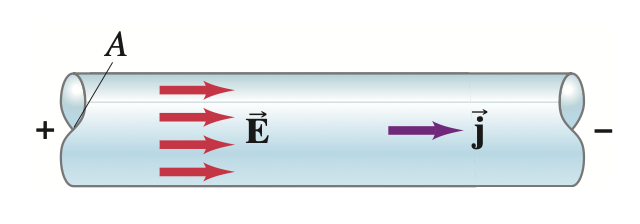
\includegraphics[scale = 0.5]{Images/Elektriciteit/MicroscopischStroom.png}
    \end{center}
    De richting van $\Vec{J}$ is gekozen volgens de stroomzin, maar in een geleider weten we dat de stroom gedragen wordt door de elektronen: ze bewegen dus eigenlijk in de met tegengestelde zin volgens $-\Vec{J}$. De elektronen voelen initieel een kracht door de aanwezigheid van het elektrisch veld en beginnen te versnellen. Hun versnelling in de tegengestelde zin van het elektrisch veld wordt de \textbf{driftsnelheid} genoemd. Deze is ongeveer gelijk omdat de elektronen constant botsen met de atomen van de draad en dus niet rechtstreeks bewegen volgens de elektronenstroom.
    \begin{center}
        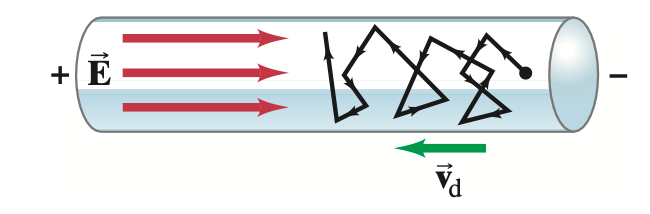
\includegraphics[scale = 0.53]{Images/Elektriciteit/Driftsnelheid.png}
    \end{center}
    Met deze nieuwe informatie kunen we de voorgaande formules herschrijven, namelijk
    \begin{equation*}
        I = \dfrac{\Delta Q}{\Delta t} = \dfrac{n(-e)Av_d\Delta t}{\Delta t} = n(-e)Av_d
    \end{equation*}
    met $v_d$ de driftsnelheid: $\sim 10^{-4} m/s$, $-e$ de lading van een elektron en $n$ het aantal ladingen per volumeeenheid. De stroomdichtheid
    \begin{equation*}
        \Vec{J} = n(-e)\Vec{v_d} = \dfrac{n(-e)^2\tau}{m_e}\Vec{E}
    \end{equation*}
    met $\tau$ de gemiddelde tijd tussen 2 botsingen, heeft dus ook het minteken wat aanduid dat in werkelijkheid de stroomzin hier in de tegengestelde richting is van de driftsnelheid van de elektronen. De betekenis van weerstand op microscopisch niveau is het verlies van energie bij botsing tussen de elektronen en de atomen van de draad, want de vibraties zorgen voor de transformatie naar warmte.
\end{app}

\begin{theo}[Weerstand en resistiviteit]{}
    De grootte van de stroom is niet enkel afhankelijk van het potentiaal, maar ook van de \textbf{weerstand}. Het wordt gegeven door de volgende formule bij Ohmse materialen (zie hierna):
    \begin{equation*}
        R = \dfrac{\Delta V}{I} 
    \end{equation*}
    De \textbf{resistiviteit} $\rho$ van een draad 
    \begin{equation*}
        R = \rho \dfrac{l}{A}
    \end{equation*}
    is recht evenredig met de lengte $l$ en omgekeerd met de doorsnede. Het is afhankelijk van het materiaal van de draad en de temperatuur van de draad. Bij metalen groeit de resistiviteit lineair met de temperatuur, in formulevorm:
    \begin{equation*}
        \rho_T = \rho_0[1+\alpha(T-T_o)]
    \end{equation*}
    De \textbf{geleidbaarheid} van een materiaal kan men beschrijven door de inverse van de resistiviteit, ofwel:
    \begin{equation*}
        \sigma = \dfrac{1}{\rho}
    \end{equation*}
    \vspace{-0.5cm}
\end{theo}

\newpage

\begin{lem}[Ohm]{Ohm}
    De stroom doorheen een draad is recht evenredig met het potentiaalverschil over de twee uiteinden, in formulevorm:
    \begin{equation*}
         I \sim \Delta V
    \end{equation*}
    Ohm ontdekte ook dat bij metalen geleiders, zogenaamde 'Ohmse' materialen,
    \begin{equation*}
         \Delta V= IR 
    \end{equation*}
    een constante bleek te zijn. Hieronder vergelijken we Ohmse materialen en niet-Ohmse materialen:
    \begin{center}
        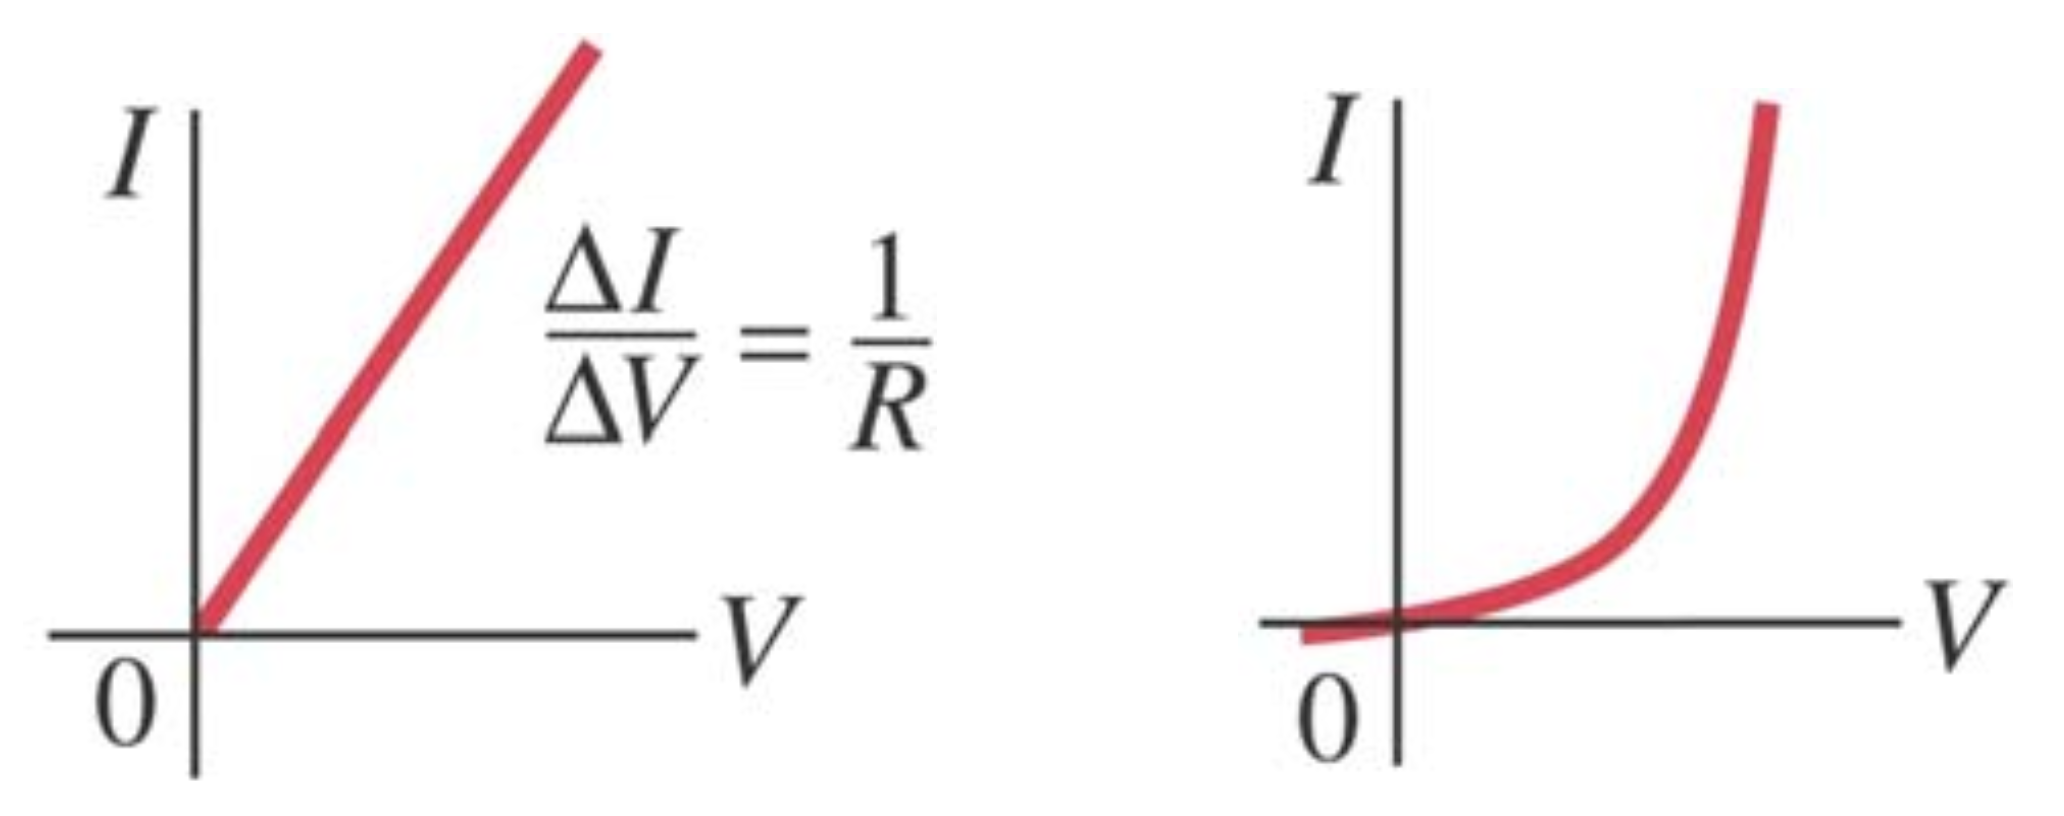
\includegraphics[scale = 0.2]{Images/Elektriciteit/GrafiekOhmseMaterialen.png}
    \end{center}
    Microscopisch zou dit betekenen dat de verhouding tussen de stroomdichtheid en het elektrische veld een constante, namelijk de \textbf{geleidbaarheid} van het materiaal, is, in formulevorm: 
    \begin{equation*}
        \Vec{J} = \sigma \Vec{E} \rightarrow \sigma = \dfrac{n(-e)^2\tau}{m_e}, \quad \rho = \dfrac{1}{\sigma} = \dfrac{m_e}{n(-e)^2\tau}
    \end{equation*}
\end{lem}

\begin{theo}[Elektrische Vermogen]{Elektrische Vermogen}
    We weten van voorgaande hoofdstukken dat vermogen een eenheid is voor arbeid per tijdseenheid: de mate waarin energie getransformeerd wordt. We vinden dus
    \begin{equation*}
        P = \dfrac{dU}{dt} = \dfrac{dq}{dt}\Delta V
    \end{equation*}
    en als we dit combineren met de definitie van stroom, bekomen we:
    \begin{equation*}
        P = I\Delta V
    \end{equation*}
    Deze formule kunnen we ook op andere manieren schrijven, namelijk:
    \begin{align*}
        P &=  I\Delta V= I(IR) = I^2R\\
        P &= I\Delta V = (\dfrac{\Delta V}{R})\Delta V = \dfrac{(\Delta V)^2}{R}
    \end{align*}
    Als we spreken over \textbf{supergeleidende} materialen, dan zijn deze volledig weerstandloos en wordt er dus geen vermogen verloren aan warmte.
\end{theo}

% \begin{app}[Elektrische geleiding in metalen, isolatoren en halfgeleiders]{Elektrische geleiding in metalen, isolatoren en halfgeleiders}

% \end{app}

% \begin{app}[Halfgeleiders en doperen]{Halfgeleiders en doperen}

% \end{app}

% \begin{app}[Halfgeleiderdiodes]{Halfgeleiderdiodes}
    
% \end{app}

% \begin{app}[Transistoren en IC’s]{Transistoren en IC’s}
    
% \end{app}




\newpage

\section{Gelijkstroomschakelingen}

\vspace{0.5cm}

\begin{theo}[Elektromotorische “kracht”]{Elektromotorische “kracht”}
    Om stroom te hebben in een circuit, hebben we een apparaat nodig dat elektrische energie kan uitgeven. Dit apparaat wordt een bron van \textbf{elektromotorische kracht} (emf) genoemd.
    Het potentiaalverschil tussen de terminalen, ofwel de klemspanning, van de bron, wanneer er geen stroom vloeit, noemt men het emf $\mathcal{E}$ van de bron. Als er nu een stroom vloeit, dan is er een interne verzwakking van de klemspanning met een mate $Ir$ waarbij $r$ de interne weerstand is. In formulevorm krijgen we:
    \begin{equation*}
        \Delta V = \mathcal{E} - Ir
    \end{equation*}

    \begin{center}
        
        \begin{minipage}{.3 \textwidth}
            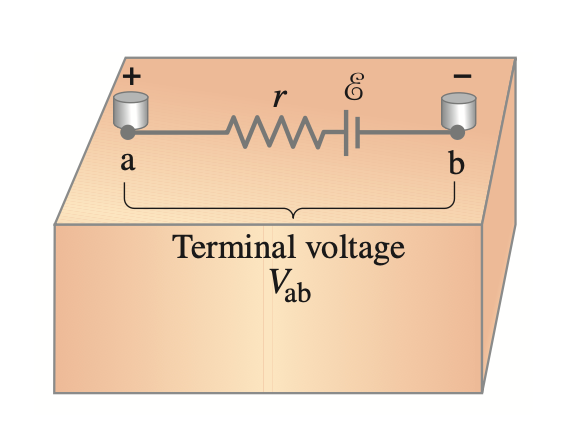
\includegraphics[scale = 0.45]{Images/Elektriciteit/Source.png}
        \end{minipage}
        \begin{minipage}{.3 \textwidth}
            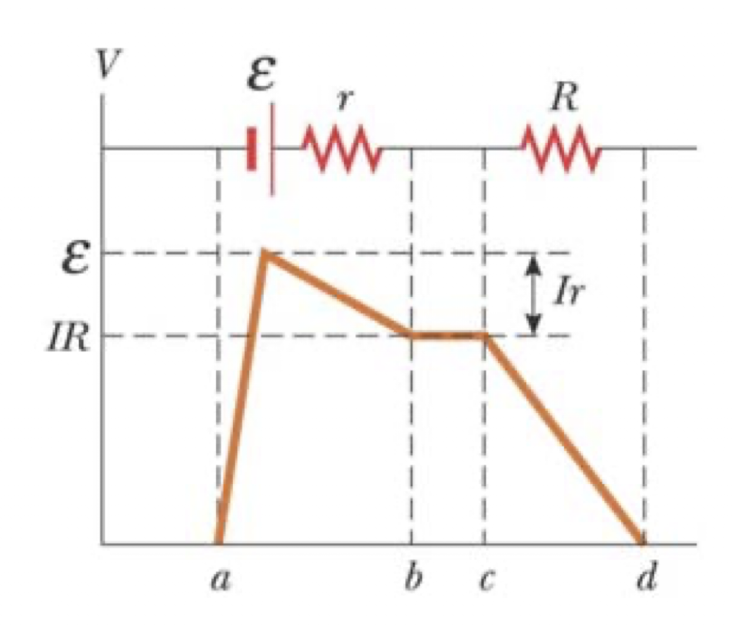
\includegraphics[scale = 0.35]{Images/Elektriciteit/EMFgrafiek.png}
        \end{minipage}

    \end{center}

    \vspace{-0.5cm}
    % \noindent \textbf{Opmerking:} de kracht in elektromotorische kracht staat niet voor een newtoniaanse kracht, het betekent eerder dat het een drijfveer is voor de elektrishe stroom.
\end{theo}

\begin{pro}[Weerstanden bij gelijkstroomschakelingen]{Weerstanden bij gelijkstroomschakelingen}
    \begin{center}
        \def\arraystretch{1.5}
        \begin{tabular}{c|c}
             Parallel & Serie \\ \hline
             $ I = \sum_i I_i $ & $ I = I_i$ \\
             $ \dfrac{1}{R} = \sum_i \dfrac{1}{R_i} $ & $R = \sum_i R_i$ \\
             $ \Delta V = \Delta V_i $ &  $ \Delta V = \sum_i \Delta V_i $
        \end{tabular}
    \end{center}
\end{pro}

% \begin{pro}[Weerstanden in serie bij gelijkstroomschakelingen]{Weerstanden in serie}
%     \begin{itemize}
%         \item $ I = I_i $
%         \item $ R = \sum_i R_i $
%         \item $ \Delta V = \sum_i \Delta V_i $
%     \end{itemize}
% \end{pro}

% \begin{pro}[Weerstanden in parallel bij gelijkstroomschakelingen]{Weerstanden in parallel}
%     \begin{itemize}
%         \item $ I = \sum_i I_i $
%         \item $ \dfrac{1}{R} = \sum_i \dfrac{1}{R_i} $
%         \item $ \Delta V = \Delta V_i $
%     \end{itemize}
% \end{pro}

\begin{theo}[Eerste regel van Kirchhoff]{Eerste regel van Kirchhoff}
     De som van de stromen die een vertakking binnenkomen, moet gelijk zijn aan de som van de stromen die de vertakking verlaten. In formulevorm:
     \begin{equation*}
         \sum I_{in} = \sum I_{uit}
     \end{equation*}
     \vspace{-0.5cm}
\end{theo}

\begin{theo}[Tweede regel van Kirchhoff]{Tweede regel van Kirchhoff}
    De som van de potentiaalverschillen over alle elementen in een gesloten kring, moet nul zijn. In formulevorm:
    \begin{equation*}
        \sum_{\text{gesloten kring}} \Delta V = 0
    \end{equation*}
    \vspace{-0.4cm}
\end{theo}

\newpage

\begin{app}[RC-kringen]{RC-kringen}
    \vspace{-0.3cm}
    \begin{minipage}{.73\textwidth}
        Als de schakelaar dicht is, dan laadt de condensator op tot het het potentiaalverschil heeft van de batterij.
        We kunnen hierop de tweede regel van Kirchhoff toepassen
        \begin{equation*}
            \mathcal{E} - \dfrac{q}{C} - IR = 0
        \end{equation*}
        waaruit volgt:
    \end{minipage}
    \begin{minipage}{.25\textwidth}
       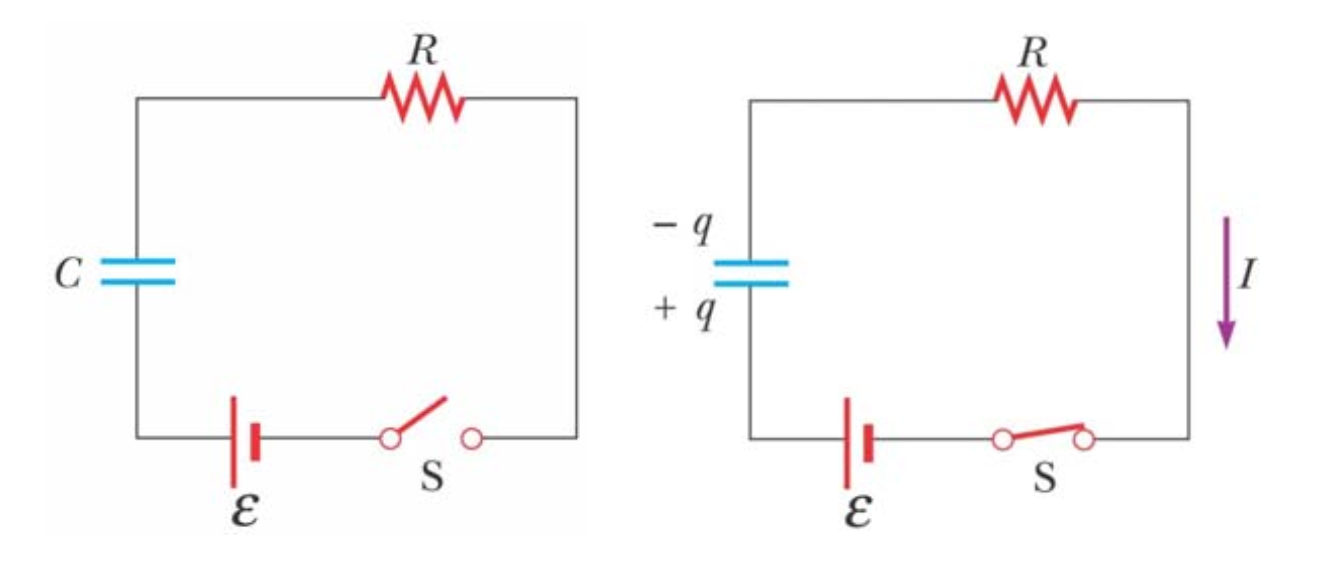
\includegraphics[scale = 0.15]{Images/Elektriciteit/RC-kring.png}
    \end{minipage}
    \vspace{-0.5cm}
    \begin{equation*}
        \mathcal{E} - \dfrac{q}{C} - \frac{dq}{dt}R = 0
    \end{equation*}
    % \begin{align*}
    %     t &= 0: \mathcal{E} - I_0R = 0 \\ 
    %     t &= \infty: \mathcal{E} - \dfrac{Q}{C} = 0.
    % \end{align*}
    \noindent Uit deze vergelijking leiden we de volgende formules voor de stroom en de ogenblikkelijke lading op de condensator af
    \begin{equation*}
        q = C\mathcal{E}\left(1-e^{-\tfrac{t}{\tau}}\right)= Q\left(1-e^{-\tfrac{t}{\tau}}\right) \ \Rightarrow \ I = \dfrac{dq}{dt} = \dfrac{\mathcal{E}}{R}e^{-\tfrac{t}{\tau}}
    \end{equation*}

    % \begin{equation*}
    %      I = \dfrac{dq}{dt} = \dfrac{d}{dt} C\mathcal{E}(1-e^{-\tfrac{t}{RC}}) = \dfrac{\mathcal{E}}{R}e^{-\tfrac{t}{RC}}
    % \end{equation*}
    % \newpage
    
    \noindent waarbij $\tau = RC$ de \textbf{tijdsconstante} die de tijd voorstelt nodig voor een condensator om tot $ 63\%$ van zijn lading en voltage te bekomen: $RC$ is een maateenheid voor de snelheid van het opladen van de condensator. \\
    \vspace{-0.2cm}

    \begin{minipage}{0.48\textwidth}
        \vspace{0.21cm}\hspace{1.4cm}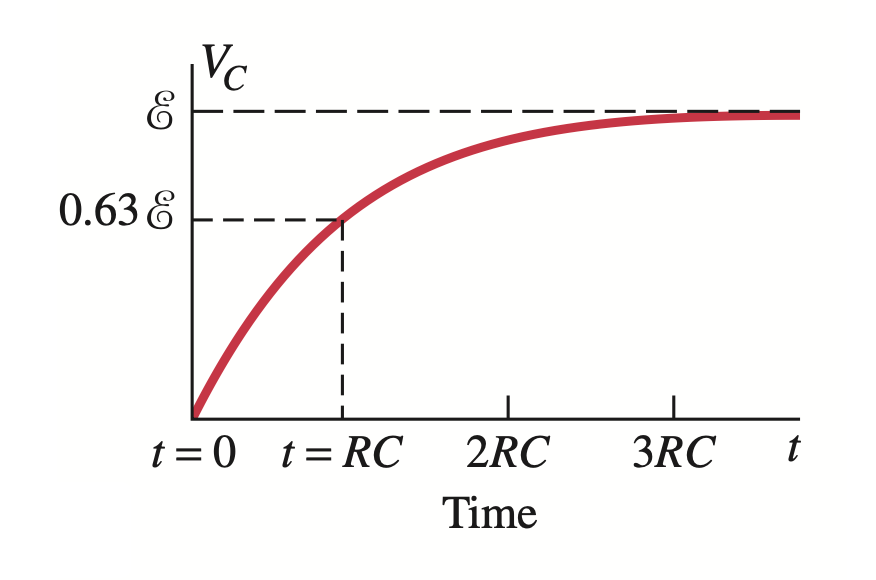
\includegraphics[scale = 0.195]{Images/Elektriciteit/Tijdsconstante1.png}
    \end{minipage}
    \begin{minipage}{0.48\textwidth}
        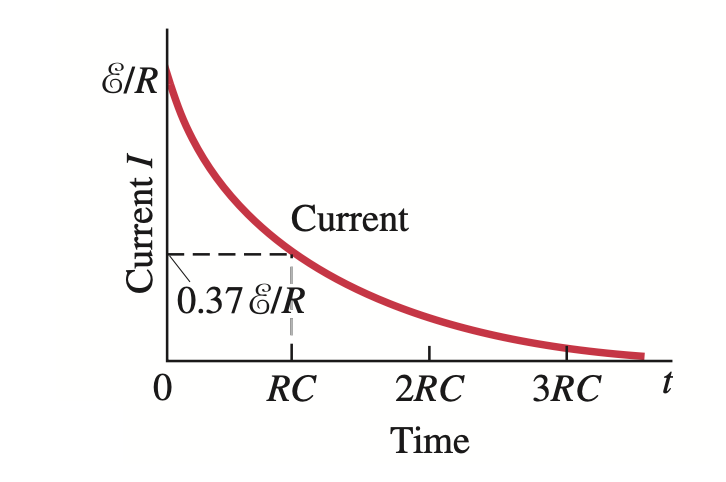
\includegraphics[scale = 0.23]{Images/Elektriciteit/Tijdsconstante2.png}
    \end{minipage}
    
    \noindent We kunnen nu de volgende formules opstellen voor de energie in de RC-kring:
    \begin{itemize}
        \item Hoeveel energie heeft de emf geleverd? 
        \begin{equation*}
            U_{\text{emf}} = \int_0^Q \mathcal{E} dq = Q\mathcal{E} = \mathcal{E}^2C
        \end{equation*}
        \item Hoeveel energie is er opgeslagen in de condensator?
        \begin{equation*}
            U_{C} = \dfrac{\mathcal{E}^2C}{2} = \dfrac{Q^2}{2C}
        \end{equation*}
        \item Hoeveel warmte is er gedisipeerd in de weerstand?
        \begin{equation*}
            U_{R} = \dfrac{\mathcal{E}^2C}{2} = \dfrac{Q^2}{2C}
        \end{equation*}
    \end{itemize}
    We zien dus dat de energie geleverd door de emf netjes is verdeeld over de weerstand en de condensator, namelijk:
    \begin{equation*}
        U_{\text{emf}} = U_{C} + U_{R}
    \end{equation*}
\end{app}



\newpage

\vspace*{\fill}
\begin{center}
    
\section*{Magnetisme}
\end{center}

\vspace*{\fill}

\newpage

\section{Magnetisme}

\begin{theo}[Magnetische velden]{Magnetische velden}
    Net zoals we rondom een elektrische lading een elektrisch veld hebben gedefinieerd, kunnen we rond een magneet een magnetisch veld
    $\Vec{B}$ definiëren. Magnetische veldlijnen op tekeningen hebben dusdanig ook dezelfde eigenschappen als elektrische veldlijnen, namelijk

    \begin{minipage}{.7\textwidth}
        \begin{itemize}
            \item de richting van het magnetische veld is tangentieel met de magnetische veldlijnen
            \item de hoeveelheid magnetische veldlijnen per oppervlakte duidt op het sterkte van het magnetische veld
        \end{itemize}

    \end{minipage}
    \begin{minipage}{.24\textwidth}
        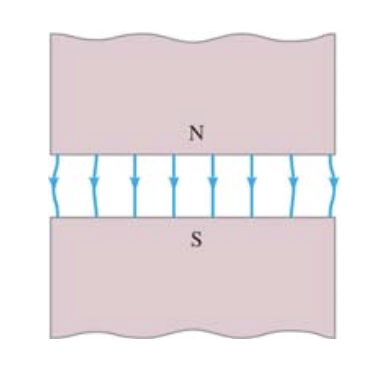
\includegraphics[scale = 0.52]{Images/Magnetisme/HomogeenMagnetischVeld}
    \end{minipage}

    \noindent Elektrische stroom \textbf{produceert} een magnetisch veld. Een niet-magnetische, geleidende draad is dus magnetisch als we er stroom op zetten.
    Om de richting van het magnetisch veld te weten, kunnen we de \textbf{rechterhandregel} toepassen.

%    \begin{minipage}{.75\textwidth}
%        "Pak de draad vast met je rechterhand en steek je duim uit in
%        de richting van de conventionele stroomzin en vouw je vingers dicht in de richting van het magnetische veld."
%    \end{minipage}
%    \begin{minipage}{.21\textwidth}
%        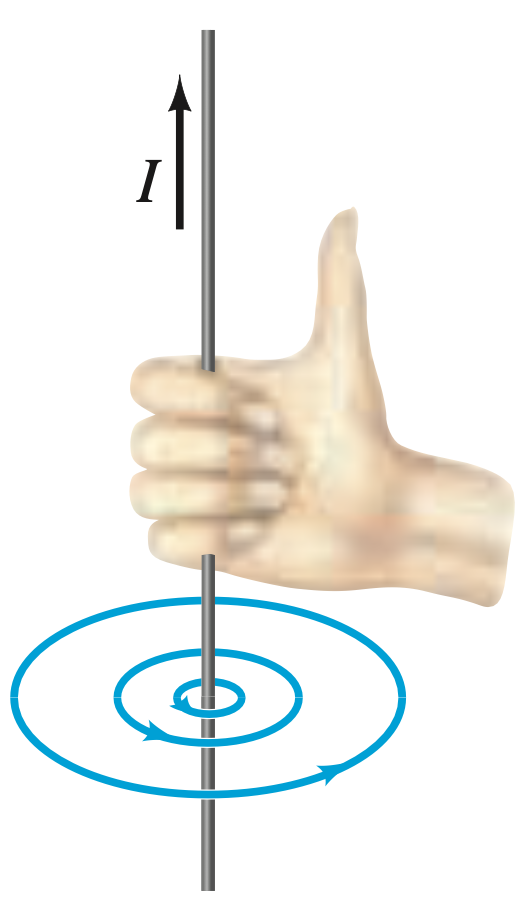
\includegraphics[scale = 0.2]{Images/Magnetisme/Rechterhandregel}
%    \end{minipage}

\end{theo}

%\begin{app}[Elekrtische stroom]{Elekrtische stroom}
%    Elektrische stroom \textbf{produceert} een magnetisch veld. Een niet-magnetische, geleidende draad is dus wel magnetisch als we er stroom op zetten.
%    Om de richting van het magnetisch veld te weten, kunnen we de \textbf{rechterhandregel} toepassen:
%
%    \begin{minipage}{.8\textwidth}
%        pak de draad vast met je rechterhand en steek je duim uit in
%        de richting van de conventionele stroomzin en vouw je vingers dicht in de richting van het magnetische veld.
%    \end{minipage}
%    \begin{minipage}{.16\textwidth}
%        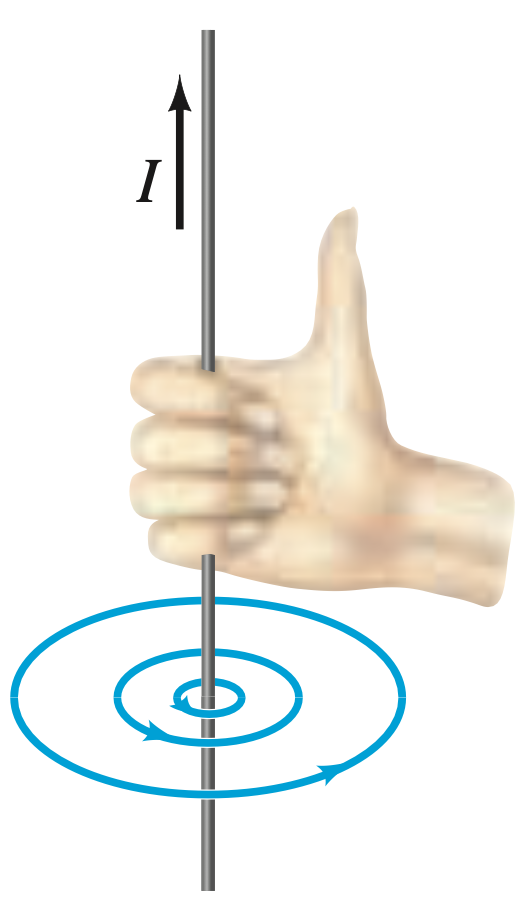
\includegraphics[scale = 0.2]{Images/Magnetisme/Rechterhandregel}
%    \end{minipage}
%\end{app}

\begin{theo}[Magnetische kracht]{Magnetische kracht}
    De relatie tussen de magnetische kracht $\Vec{F}$ van een draad met stroom $I$ en het magnetisch veld $\Vec{B}$ kan geschreven worden als een vector product
    \begin{equation*}
        d\Vec{F}= Id\Vec{\ell} \times \Vec{B}
    \end{equation*}
    waarbij $d\Vec{F}$ een infinitesimale kracht op een infinitesimale lengte $d\Vec{\ell}$ van de draad in het magnetische veld.
    \begin{center}
        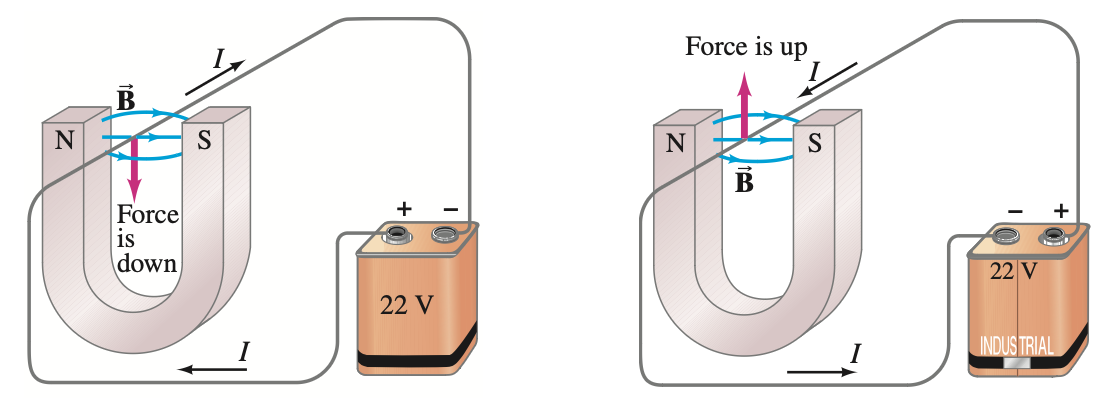
\includegraphics[scale = 0.45]{Images/Magnetisme/MagnetischeKracht}
    \end{center}
    \begin{minipage}{.75\textwidth}
        Als het veld homogeen is, dan zal elk infinitesimaal deeltje $d\Vec{\ell}$ van de rechte draad dezelfde hoek maken met het magnetische veld $\Vec{B}$.
        Hieruit volgt dan de formule:
        \begin{equation*}
            \Vec{F} = I\Vec{\ell} \times \Vec{B}
        \end{equation*}
    \end{minipage}
    \begin{minipage}{.21\textwidth}
        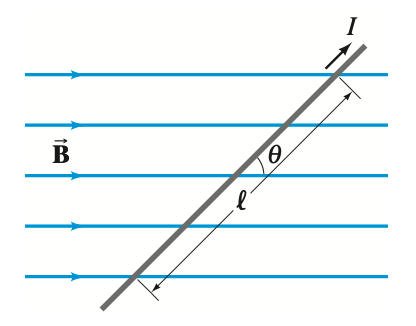
\includegraphics[scale = 0.25]{Images/Magnetisme/DraadHomogeenVeld}
    \end{minipage}
\end{theo}

%\begin{app}[Magnetische kracht in een homogeen veld]{Magnetische kracht in een homogeen veld}
%    \vspace{-0.5cm}
%    \begin{minipage}{.75\textwidth}
%        Als het veld homogeen is, dan zal elk infinitesimaal deeltje $d\Vec{\ell}$ dezelfde hoek maken met het magnetische veld $\Vec{B}$.
%        Hieruit volgt dan de formule:
%        \begin{equation*}
%            \Vec{F} = I\Vec{\ell} \times \Vec{B}
%        \end{equation*}
%    \end{minipage}
%    \begin{minipage}{.21\textwidth}
%        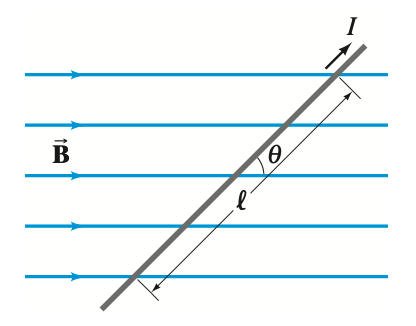
\includegraphics[scale = 0.25]{Images/Magnetisme/DraadHomogeenVeld}
%    \end{minipage}
%\end{app}

%\begin{ex}[Willekeurige stroomvoerende geleider in een homogeen magnetisch veld]{Willekeurige stroomvoerende geleider in een homogeen magnetisch veld}
%    \begin{minipage}{.6\textwidth}
%        \vspace{-0.5cm}
%        \begin{align*}
%            \Vec{F} &= I\int_a^{b}d\Vec{l} \times \Vec{B} \\
%            &= I(\int_a^{b}d\Vec{l} \times \Vec{B}) \quad \text{(B is homogeen)} \\
%            &= I(\Vec{L} \times \Vec{B})
%        \end{align*}
%    \end{minipage}
%    \begin{minipage}{.36\textwidth}
%        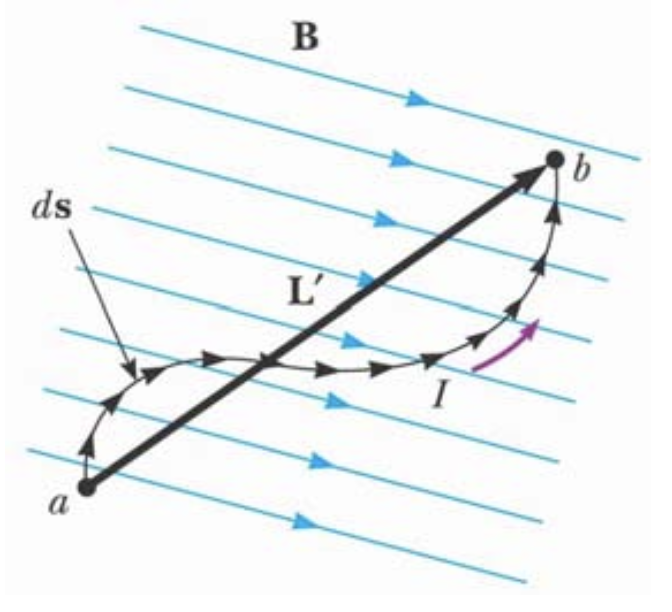
\includegraphics[scale = 0.35]{Images/Magnetisme/StroomvoerendeGeleiderHomogeenMagnetischVeld}
%    \end{minipage}
%\end{ex}


\newpage

\begin{theo}[Magnetische kracht op een bewegende lading]{Magnetische kracht op een bewegende lading}
    Elektrische stroom is een verzameling van N bewegende ladingen, we kunnen de definitie van magnetische kracht dus ook anders schrijven
    \begin{equation*}
        \Vec{F} = I\Vec{\ell} \times \Vec{B} = Nq\Vec{v} \times \Vec{B}
    \end{equation*}
    sinds $I = \tfrac{Nq}{t}$ en $\Vec{\ell} = \Vec{v}t$. De bijlage hieronder toont de magnetische kracht op bewegende ladingen:
    \begin{center}
        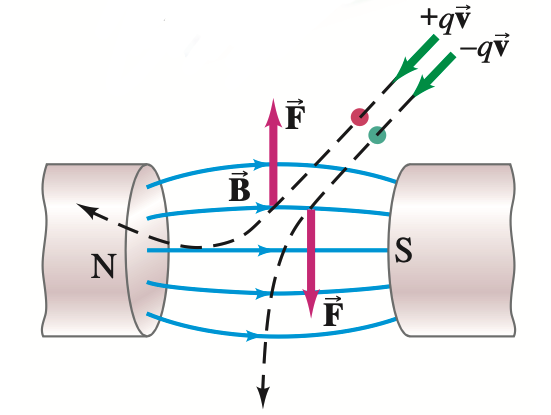
\includegraphics[scale=0.25]{Images/Magnetisme/MagnetischeKrachtOpBewgendeLading}
    \end{center}
\end{theo}

\begin{vrg}[Verschillen tussen elektrische en magnetische kracht]{Verschillen tussen elektrische en magnetische kracht}
    \vspace{-0.3cm}
    \def\arraystretch{2}
    \hspace{-0.35cm}
    \begin{tabular}{c|c}
        Elektrische kracht: $\Vec{F} = q\Vec{E}$ & Magnetische kracht: $\Vec{F} = q\Vec{v} \times \Vec{B}$ \\ \hline
        in de \textbf{richting} van het elektrsich veld & \textbf{loodrecht} op het magnetische veld \\
        werkt op een \textbf{lading} & werkt op een \textbf{bewegende lading} \\
        levert \textbf{arbeid} bij de verplaatsing van de lading & levert \textbf{geen arbeid} bij de verplaatsing van de lading \\
    \end{tabular}
\end{vrg}

\begin{app}[Bewegende lading in een vlak loodrecht op magnetisch veld]{Bewegende lading in een vlak loodrecht op magnetisch veld}
    \begin{minipage}{.67\textwidth}
        Het pad van een bewegende lading in een vlak loodrecht op het magnetisch veld is cirkelvormig.
        De kracht zal altijd loodrecht zijn op de snelheid, dus de lading zal cirkelvormig bewegen met
        centripetale versnelling:
        \begin{equation*}
            a_{R} = \dfrac{v^2}{r}.
        \end{equation*}
        De periode heeft de volgende formule:
        \begin{equation*}
            T = \dfrac{2\pi r}{v} = \dfrac{2\pi m}{qB} = \dfrac{1}{f}
        \end{equation*}
        sinds $r = \tfrac{mv}{qB}$.
    \end{minipage}
    \begin{minipage}{.29\textwidth}
        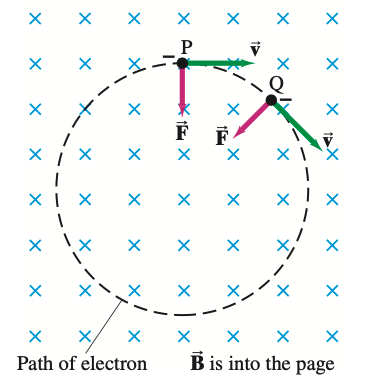
\includegraphics[scale = 0.35]{Images/Magnetisme/CirkelvormigeBewegingMagentischVeld}
    \end{minipage}
\end{app}

\newpage

\begin{theo}[Magnetisch dipool moment]{Magnetisch dipool moment}
    Wanneer een lading stroomt door een gesloten kring in een extern magnetisch veld, dan kan de magnetische kracht torsie veroorzaken.
    Stroom vloeit door de rechthoekige kring (zie figuur a), waarvan we aannemen dat hij parrallel is met het veld $\Vec{B}$.
    Het veld oefent noch een kracht, noch een krachtmoment 

    \vspace{-0.3cm}
%    \newpage
    % \Vec{\tau} = \Vec{r} \times \Vec{F} = \Vec{r} \times \Vec{F_1} + \Vec{r} \times \Vec{F_2}
    \hspace{-0.5cm}\begin{minipage}{0.79\textwidth}
        uit op de horizontale delen; hier is $\sin(\theta) = 0$. Het veld oefent wel een kracht uit op de verticale delen
        (zie figuur b), we noemen deze krachten $\Vec{F_1}$ en $\Vec{F_2}$. Deze krachten zorgen voor een krachtmoment:
        % \vspace{-0.2cm}
        % \begin{equation*}
        %     \tau = IaB\dfrac{b}{2} + IaB\dfrac{b}{2} = IabB = IAB
        % \end{equation*}
        \begin{equation*}
            \Vec{\tau} = NI(\Vec{a} \times \Vec{b}) \times \Vec{B} = NI\Vec{A} \times \Vec{B}
        \end{equation*}
        waarbij $\Vec{A} = \Vec{a} \times \Vec{b}$ de oppervlakte van de spoel en $I = NI$ in een spoel met $N$ kringen.
        % Als de spoel $N$ kringen heeft en een hoek $\theta$ maakt met het magnetisch veld (zie figuur c),
        % dan is de stroom $NI$ en volgt:
        % \begin{equation*}
        %     \Vec{\tau} = NI\Vec{A} \times \Vec{B}
        % \end{equation*}
        % want de krachten blijven gelijk, maar de krachtarmen verkleint.
        Het \textbf{magnetisch dipool moment} $\Vec{\mu}$ wordt als volgt gedefinieerd:
        \begin{equation*}
            \Vec{\mu} = NI\Vec{A}
        \end{equation*}
        waarbij de ricthing van $\Vec{A}$ loodrecht is op het vlak van de spoel. Hiermee kunnen we de krachtmoment formule herschrijven:
        \begin{equation*}
            \Vec{\tau} = \Vec{\mu} \times \Vec{B}
        \end{equation*}
        De potentiële energie U kunnen we dan als volgt berekenen
        \begin{equation*}
            U = \int_0^{\tfrac{\pi}{2}} \tau d\theta = \mu B \int_0^{\tfrac{\pi}{2}} \sin(\theta) d\theta = -\mu B\cos(\theta) = -\Vec{\mu} \cdot \Vec{B}
        \end{equation*}
        
    \end{minipage}
    \begin{minipage}{.17\textwidth}
        \vspace{0.5cm}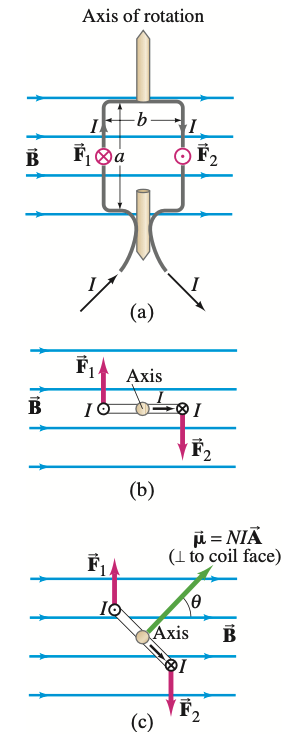
\includegraphics[scale = 0.32]{Images/Magnetisme/MagnetischDipoolMoment}
    \end{minipage}
    % \vspace{0.2cm} \\
    \vspace{-0.1cm}\\
    wat ook logisch is sinds we dit kunnen vergelijkigen met het elektrisch dipool moment.
\end{theo}

\begin{vrg}[Verschillen tussen het magnetisch en elektrisch dipoolmoment]{Verschillen tussen het magnetisch en elektrisch dipoolmoment}
    \vspace{-0.3cm}
    \def\arraystretch{2}
    \centering
    \begin{tabular}{c|c}
       Magnetisch dipoolmoment in een magnetisch veld & Elektrisch dipolmoment in een elektrisch veld \\ \hline
        $\Vec{\tau} = \Vec{\mu} \times \Vec{B}$ & $\Vec{\tau} = \Vec{p} \times \Vec{E}$ \\ 
        $U = -\Vec{\mu} \cdot \Vec{B}$ & $U = -\Vec{p} \cdot \Vec{E}$ \\
    \end{tabular}
    \vspace{-0.2cm}
\end{vrg}

\begin{app}[Magnetisch moment van een atoom]{Magnetisch moment van een atoom}
    Bij een atoom cirkelt een elektron rond de kern: er is dus een stroom. We vinden hiervoor:
    \begin{equation*}
        I = \dfrac{e}{T} = \dfrac{e\omega}{2\pi} = \dfrac{ev}{2\pi r}
    \end{equation*}
    We kunnen ook het \textbf{orbitaal magnetisch moment} berekenen, namelijk: 
    \begin{equation*}
        \Vec{\mu} = I\Vec{A} = \dfrac{ev}{2\pi r} \pi r^{2} \hat{k} = -\dfrac{e}{2m_{e}}(-m_{e}rv\hat{k}) = -\dfrac{e}{2m_{e}}\Vec{L}
    \end{equation*}
    Hierbij hebben we dus het magnetisch moment van een atoom uitgedrukt in termen van het impulsmoment. 
    % Het feit dat de zin tegengesteld is, is logisch, want de zin van het impulsmoment wordt bepaald door de zin van de snelheidsvector.
    % De conventionele stroomzin is, daarentegen, tegengesteld aan de beweging van een elektron.
    \vspace{0cm}
\end{app}

\newpage


\begin{theo}[Hall-Effect]{Hall-Effect}
    Wanneer een stroomvoerende geleider in een magnetisch veld wordt vastgehouden,
    oefent het veld een zijwaartse kracht uit op de ladingen die in de geleider bewegen.
    De lading zal kaatsen en er zal een potentiaalverschil ontstaan. Dit potentiaalverschil zal
    stijgen totdat het gecreërde elektrisch veld $\Vec{E}_H$ een kracht $e\Vec{E}_H$ op de ladingen uitoefent dat gelijk en tegengesteld is aan de magnetische kracht, ofwel:
    \begin{minipage}{0.76\textwidth}
        % Wanneer een stroomvoerende geleider in een magnetisch veld wordt vastgehouden,
        % oefent het veld een zijwaartse kracht uit op de ladingen die in de geleider bewegen.
        % De lading zal kaatsen en er zal een potentiaalverschil ontstaan. Dit potentiaalverschil zal
        % stijgen totdat het gecreërde elektrisch veld $\Vec{E}_H$ een kracht $e\Vec{E}_H$
        % op de ladingen uitoefent dat gelijk en tegengesteld is aan de magnetische kracht, ofwel:

        \vspace{0.1cm}

        \begin{equation*}
            eE_H = ev_{d}B \Rightarrow E_H = v_{d}B
        \end{equation*}
        Dit noemen we het \textbf{Hall-effect}. Het potentiaalverschil wordt ook wel de \textbf{Hallsspanning}
        en wordt bij een uniform Hall veld in een lange, dunne geleider gegeven door
        \begin{equation*}
            \mathcal{E}_H = E_{H}d = v_{d}Bd = R_H\dfrac{IBd}{A}
        \end{equation*}
        met $R_H = \tfrac{1}{ne}$ de \textbf{Hall-coëfficiënt}. Hieruit zien we ook dat er een snelheid
        nodig is om rechtlijnig door de geleider te gaan, namelijk
        \begin{equation*}
            v = \dfrac{E_H}{B} = R_H\dfrac{I}{A}
        \end{equation*}
        dit zal in volgende toepassing van groot belang zijn.    
    \end{minipage}
    \begin{minipage}{.20\textwidth}
        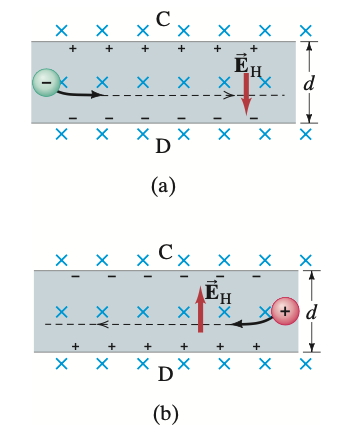
\includegraphics[scale = 0.3]{Images/Magnetisme/HallEffect}
    \end{minipage} 
\end{theo}

% \begin{summ}[Rechterhandregels]{Rechterhandregels}
%     \centering
%     \includegraphics[scale=0.45]{Images/Magnetisme/RechterhandRegels}
% \end{summ}

\begin{app}[Massaspectrometer]{Massaspectrometer}
    \begin{minipage}{.7\textwidth}
        De massaspectrometer is een toestel dat gebruikt wordt om de massas van atomen te meten.
        Ionen worden geproduceerd door warmte of door een stroom in de bron $S$.  De partikels, met massa $m$ en elektrische lading $q$, 
        gaan door de gleuf $S_{1}$ en gaan door het gebied waar elektrisch veld en magnetisch veld elkaar kruisen. We weten dat 
        het Halleffect nu op het partikel een effect zal hebben en dus weten we ook de snelheid die nodig is om door de gleuf $S_{2}$ 
        te geraken. Dit is dus eigenlijk wat men noemt een \textbf{snelheidsfilter}. 
        In het halfcirkelvormig gebied is er enkel een magnetisch veld $B'$ en zal dus het magnetisch veld voor een cirkelvormige beweging veroorzaken voor het partikel. 
        De straal $r$ van dit cirkelvormig pad kunnen we vinden door te plaats te meten waar het partikel aankomt. Volgens de tweede wet van Newton krijgen we nu 
    \end{minipage}
    \begin{minipage}{.28\textwidth}
        \vspace{-0.25cm}
        \includegraphics[scale = 0.5]{Images/Magnetisme/Massaspectrometer.png}
    \end{minipage}
    \vspace{0.25cm}

    \begin{equation*}
        m = \dfrac{qB'r}{v} = \dfrac{qBB'r}{E}
    \end{equation*}
    en kunnen we $m$ nu dus bepalen.
\end{app}

\newpage

\section{Bronnen van magnetische velden}

\begin{theo}[Magnetisch veld ten gevolge van een rechte draad]{Magnetisch veld ten gevolge van een rechte draad}
    \begin{minipage}{0.87\textwidth}
        Het magnetische veld ten gevolge van de elektrische stroom in een lange rechte draad is zodanig dat de
        veldlijnen cirkels zijn met de draad in het midden (zie figuur). De veld sterkte is groter hoe dichter je bij de
        draad bent en hoe groter de stroom, in formulevorm:
        \begin{equation*}
            B \propto \dfrac{I}{r}
        \end{equation*}
        met r de loodrechte afstand van de draad. Deze relatie blijft waar als we aanemen dat de draad lang is.
        Het magnetisch veld nabij een lange, rechte draad is als volgt
        \begin{equation*}
            B = \dfrac{\mu_0}{2\pi}\dfrac{I}{r}
        \end{equation*}
        met $\mu_0$ de magnetische permeabiliteit in vacuum.
    \end{minipage}
    \begin{minipage}{.09\textwidth}
        \includegraphics[scale=0.225]{Images/Magnetisme/MagnetischVeldTenGevolgeRechteDraad}
    \end{minipage}
\end{theo}

\begin{app}[Magnetische kracht tussen twee parallelle draden]{Magnetische kracht tussen twee parallelle draden}
    \begin{minipage}{0.77\textwidth}
        Neem twee lange evenwijdige draden gescheiden door een afstand d, zoals in de figuur. Ze voeren respectievelijk stromen $I_1$ en $I_2$.
        Elke stroom produceert een magnetisch veld dat door de ander wordt ‘gevoeld’, dus oefenen ze een kracht uit op mekander. We weten dat
        \begin{equation*}
            F_{\text{max}} = I\ell B
        \end{equation*}
        en dus krijgen we:
        \begin{equation*}
            F = I_{2}B_{1}\ell_{2} = \dfrac{\mu_0}{2\pi}\dfrac{I_{1}I_{2}}{d}\ell_{2}
        \end{equation*}
    \end{minipage}
    \begin{minipage}{.19\textwidth}
        \includegraphics[scale=0.225]{Images/Magnetisme/MagnetischeKrachtTussenTweeParallelleDraden}
    \end{minipage} \vspace{0.2cm}\\
    Hieruit kunnen we afleiden dat evenwijdige stroomvoerende geleiders elkaar
    \begin{itemize}
        \item aantrekken indien de stroom in dezelfde richting vloeit,
        \item afstoten indien de stroom in tegengestelde richting vloeit.
    \end{itemize}
\end{app}

\begin{lem}[Ampère]{Ampère}
    \vspace{-0.75cm}\begin{minipage}{0.79\textwidth}
        De lijnintegraal van het magneetveld langs een gesloten pad is gelijk aan $\mu_{0}I_{\text{in}}$, waarbij $I_{\text{in}}$ de totale stroom is, die vloeit door een oppervlak dat omsloten is door het pad, in formulevorm:
        \begin{equation*}
            \oint \Vec{B} \cdot d\Vec{\ell} = \mu_{0}I_{\text{in}}
        \end{equation*}
    \end{minipage}
    \begin{minipage}{.17\textwidth}
        \includegraphics[scale=0.3]{Images/Magnetisme/WetVanAmpere}
    \end{minipage}
\end{lem}

\newpage

\begin{theo}[Het magnetisch veld van een spoel]{Het magnetisch veld van een spoel}
    Een lange draad met meerdere windingen noemen we een \textbf{spoel}, zie de figuren hieronder.

%    \vspace{0.5cm}

%    \begin{minipage}{.48\textwidth}
        \begin{center}
%            Spoel: \\
            \includegraphics[scale = 0.4]{Images/Magnetisme/Spoel}
        \end{center}
%    \end{minipage}
%    \begin{minipage}{.48\textwidth}
%        \begin{center}
%            \vspace{0.75cm}
%            Dicht gepakte spoel: \\
%            \includegraphics[scale = 0.25]{Images/Magnetisme/SpoelDicht}
%        \end{center}
%    \end{minipage}

%    \vspace{0.5cm}

    \noindent Elke winding genereert een magnetisch veld. Nabij elke draad zijn de veldlijnen quasi cirkels,
    net zoals bij een rechte draad. In het centrum van de spoel is het netto magnetisch veld een redelijk
    groot en redelijk uniform veld, we nemen aan dat een spoel dicht gebonden is en dus dat het veld praltisch uniform is.
    We kunnen de wet van Ampère toepassen op de zijden van de rechthoek (zie figuur onderaan)
    \begin{align*}
%        \hspace{1cm}
        \oint \Vec{B} \cdot d\Vec{\ell} &= \int_{a}^{b} \Vec{B} \cdot d\Vec{\ell} + \int_{b}^{c} \Vec{B} \cdot d\Vec{\ell}
        +  \int_{c}^{d} \Vec{B} \cdot d\Vec{\ell} +  \int_{d}^{a} \Vec{B} \cdot d\Vec{\ell} \\
                                        &= \int_{b}^{c} \Vec{B} \cdot d\Vec{\ell}  \\
                                        &= B\ell
    \end{align*}
    waarbij de integralen op de paden $a \to b$, $b \to c$ en $d \to a$ nul zijn, want het veld is praktisch nul tussen in en buiten de spoel.
    We berkenen nu de formule van het magnetisch veld van een spoel:
    \begin{align*}
        \oint \Vec{B} \cdot d\Vec{\ell} &= \mu_{0}NI \\
        B\ell &=  \mu_{0}NI \\
        B &=  \mu_{9}nI
    \end{align*}
    met $n= \tfrac{N}{\ell}$ het aantal windingen per lengte.
    \begin{center}
        \includegraphics[scale = 0.3]{Images/Magnetisme/SpoelMagnetischVeld}
    \end{center}
\end{theo}

\end{document}
